\documentclass[a4paper,10pt,BCOR10mm,oneside,headsepline]{scrbook}


%\usepackage[spanish]{babel}
 
\usepackage{graphicx}
\usepackage{polyglossia}
\setmainlanguage{spanish} % Idioma principal
\usepackage{amssymb,amsmath}
\usepackage{fontspec}
%\usepackage[utf8]{inputenc}
\usepackage{wasysym}% provides \ocircle and \Box
\usepackage{enumitem}% easy control of topsep and leftmargin for lists 
\usepackage{smartdiagram}
\usepackage{mathrsfs} 
\usepackage{color}% used for background color
\usepackage{forloop}% used for \Qrating and \Qlines
\usepackage{ifthen}% used for \Qitem and \QItem
\usepackage{typearea}
\usepackage{hyperref}
%\areaset{17cm}{26cm}
%\%setlength{\topmargin}{3cm}
%\usepackage{scrpage2}
\usepackage{fancyhdr}
\usepackage{appendix}
%\pagestyle{scrheadings}
%\ihead{Encuesta sobre Lic. en Matemática UNRC}
%\ohead{\pagemark}
%\chead{}
%\cfoot{}
\usepackage{tikz}
\usetikzlibrary{backgrounds}
\usetikzlibrary{trees,positioning,arrows}
\usetikzlibrary{mindmap}
\setsansfont{Roboto Condensed}
\renewcommand{\familydefault}{\sfdefault}
\DeclareMathOperator{\anti}{\mathfrak{so}}
\DeclareMathOperator{\SO}{SO}


%%%%%%%%%%%%Configuracion Apéndices %%%%%%%%%%%%%%%%%%%%%%%%55555  
\AtBeginEnvironment{subappendices}{%
\chapter*{Apéndices}
\addcontentsline{toc}{chapter}{Apéndices}
\counterwithin{figure}{section}
\counterwithin{table}{section}
}

%%%%%%%%%%%%%%%%%%%%%%%%%%%%%%%%%%%%%%%%%%%%%%%%%%%%%%%%%%%%
%% Beginning of questionnaire command definitions %%
%%%%%%%%%%%%%%%%%%%%%%%%%%%%%%%%%%%%%%%%%%%%%%%%%%%%%%%%%%%%
%%
%% 2010, 2012 by Sven Hartenstein
%% mail@svenhartenstein.de
%% http://www.svenhartenstein.de
%%
%% Please be warned that this is NOT a full-featured framework for
%% creating (all sorts of) questionnaires. Rather, it is a small
%% collection of LaTeX commands that I found useful when creating a
%% questionnaire. Feel free to copy and adjust any parts you like.
%% Most probably, you will want to change the commands, so that they
%% fit your taste.
%%
%% Also note that I am not a LaTeX expert! Things can very likely be
%% done much more elegant than I was able to. If you have suggestions
%% about what can be improved please send me an email. I intend to
%% add good tipps to my website and to name contributers of course.
%%
%% 10/2012: Thanks to karathan for the suggestion to put \noindent
%% before \rule!

%% \Qq = Questionaire question. Oh, this is just too simple. It helps
%% making it easy to globally change the appearance of questions.
\newcommand{\Qq}[1]{\textbf{#1}}

%% \QO = Circle or box to be ticked. Used both by direct call and by
%% \Qrating and \Qlist.
\newcommand{\QO}{$\Box$}% or: $\ocircle$

%% \Qrating = Automatically create a rating scale with NUM steps, like
%% this: 0--0--0--0--0.
\newcounter{qr}
\newcommand{\Qrating}[1]{\QO\forloop{qr}{1}{\value{qr} < #1}{---\QO}}

%% \Qline = Again, this is very simple. It helps setting the line
%% thickness globally. Used both by direct call and by \Qlines.
\newcommand{\Qline}[1]{\noindent\rule{#1}{0.6pt}}

%% \Qlines = Insert NUM lines with width=\linewith. You can change the
%% \vskip value to adjust the spacing.
\newcounter{ql}
\newcommand{\Qlines}[1]{\forloop{ql}{0}{\value{ql}<#1}{\vskip0em\Qline{\linewidth}}}

%% \Qlist = This is an environment very similar to itemize but with
%% \QO in front of each list item. Useful for classical multiple
%% choice. Change leftmargin and topsep accourding to your taste.
\newenvironment{Qlist}{%
\renewcommand{\labelitemi}{\QO}
\begin{itemize}[leftmargin=1.5em,topsep=-.5em]
}{%
\end{itemize}
}

%% \Qtab = A "tabulator simulation". The first argument is the
%% distance from the left margin. The second argument is content which
%% is indented within the current row.
\newlength{\qt}
\newcommand{\Qtab}[2]{
\setlength{\qt}{\linewidth}
\addtolength{\qt}{-#1}
\hfill\parbox[t]{\qt}{\raggedright #2}
}

%% \Qitem = Item with automatic numbering. The first optional argument
%% can be used to create sub-items like 2a, 2b, 2c, ... The item
%% number is increased if the first argument is omitted or equals 'a'.
%% You will have to adjust this if you prefer a different numbering
%% scheme. Adjust topsep and leftmargin as needed.
\newcounter{itemnummer}
\newcommand{\Qitem}[2][]{% #1 optional, #2 notwendig
\ifthenelse{\equal{#1}{}}{\stepcounter{itemnummer}}{}
\ifthenelse{\equal{#1}{a}}{\stepcounter{itemnummer}}{}
\begin{enumerate}[topsep=2pt,leftmargin=2.8em]
\item[\textbf{\arabic{itemnummer}#1.}] #2
\end{enumerate}
}

%% \QItem = Like \Qitem but with alternating background color. This
%% might be error prone as I hard-coded some lengths (-5.25pt and
%% -3pt)! I do not yet understand why I need them.
\definecolor{bgodd}{rgb}{0.8,0.8,0.8}
\definecolor{bgeven}{rgb}{0.9,0.9,0.9}
\newcounter{itemoddeven}
\newlength{\gb}
\newcommand{\QItem}[2][]{% #1 optional, #2 notwendig
\setlength{\gb}{\linewidth}
\addtolength{\gb}{-5.25pt}
\ifthenelse{\equal{\value{itemoddeven}}{0}}{%
\noindent\colorbox{bgeven}{\hskip-3pt\begin{minipage}{\gb}\Qitem[#1]{#2}\end{minipage}}%
\stepcounter{itemoddeven}%
}{%
\noindent\colorbox{bgodd}{\hskip-3pt\begin{minipage}{\gb}\Qitem[#1]{#2}\end{minipage}}%
\setcounter{itemoddeven}{0}%
}
}
\title{Resumen actividades 2017-2021}
\author{\textbf{Proyecto PIIMEI para Lic. en Matemática.}\\
%\author{
Marcelo Ruiz,
Albina Priori,
David Ferreyra,
Agustina Gonzalez,
Mara Rossani,\\
Stefania Demaria,
Graciela Giubergia,
Valentina Orquera,
Noelia Matos,\\
Valentín Cassano,
Fernando Mazzone}
\date{}
%%%%%%%%%%%%%%%%%%%%%%%%%%%%%%%%%%%%%%%%%%%%%%%%%%%%%%%%%%%%
%% End of questionnaire command definitions %%
%%%%%%%%%%%%%%%%%%%%%%%%%%%%%%%%%%%%%%%%%%%%%%%%%%%%%%%%%%%%

\pagestyle{fancyplain}

 \renewcommand{\sectionmark}[1]
                 {\markright{\thesection\ #1}}


% \lhead[\fancyplain{}{\bfseries\thepage}]
%       {\fancyplain{}{\bfseries\rightmark}}
%
 \rhead[\fancyplain{}{\bfseries\leftmark}]{\fancyplain{}{\bfseries\thepage}}




 \lhead[\fancyplain{}{\vspace{-2cm}
\includegraphics[scale=1]{membrete2022.pdf}}]{\fancyplain{}{\vspace{-2cm}
\includegraphics[scale=.7]{membrete2022.pdf}}}

\cfoot{}









\begin{document}


\hyphenation{in-de-pen-dien-te}

\maketitle
\normalfont
\tableofcontents

\chapter{Actividades Investigación Evaluativa Licenciatura en Matemática}

\section{Estudio de informes y documentos de organismos nacionales e internacionales}
Una de las principales consignas que presupone el proyecto PIIMEI que lleva a cabo nuestra Facultad: “ABORDAJE INTEGRADO PARA LA INNOVACIÓN CURRICULAR DE LAS CARRERAS DE EXACTAS” aprobado por Resolución Rectoral N° 450/18, es el análisis de la contextualización del plan de estudios tanto en sus aspectos formales como ocultos. Entendemos que uno de los contextos en donde la carrera actúa lo podríamos definir como el contexto internacional. Nuestros egresados han emprendido carreras en otras instituciones de Argentina y del mundo. Por tanto, nos pareció oportuno tomar en consideración la opinión de organismos nacionales, extranjeros e internacionales sobre los planes de estudios de las carreras de Lic. en Matemática. En esta dirección hay varios antecedentes intentando definir estándares, en cuanto a lo que concierne a contenidos disciplinares como a competencias profesionales. A continuación se enumera los que se han estudiado en el marco del proyecto PIIMEI.

\begin{enumerate}
 \item \emph{Proyecto Tuning América Latina}  
 
 <<El proyecto Tuning América Latina busca "afinar" las estructuras educativas de América Latina iniciando un debate cuya meta es identificar e intercambiar información y mejorar la colaboración entre las instituciones de educación superior para el desarrollo de la calidad, efectividad y transparencia. Es un proyecto independiente, impulsado y coordinado por Universidades de distintos países, tanto latinoamericanos como europeos... Participan más de 230 académicos y responsables de educación superior de Latinoamerica (Argentina, Bolivia, Brasil, Colombia, Costa Rica, Cuba, Chile, Ecuador, El Salvador, Guatemala, Honduras, México, Nicaragua, Panamá, Paraguay, Perú, Uruguay y Venezuela) y Europa (Alemania, Bélgica, Dinamarca, Eslovenia, España, Francia, Grecia, Irlanda, Italia, Lituania, Países Bajos, Portugal y Rumania). Conformados en 16 redes de áreas temáticas y 1 una red de Responsables de Política Universitaria.>>  
 
 \begin{flushright} (\href{http://www.tuningal.org/}{http://www.tuningal.org/} )
  
 \end{flushright}

 Cabe destacar que representantes de nuestra facultad  han participado de este proyecto. 
Se comprenden muchas carreras, en particular para matemática se han informado los resultados alcanzados en el siguiente documento que fue estudiado por la CCP de Matemática.
 
 \begin{itemize}
  \item  \emph{Educación Superior en América Latina: reflexiones y perspectivas en Matemáticas } María José Arroyo Paniagua (editora). 
  
 \end{itemize}

\item \emph{El informe de SIAM sobre la matemática en la industria.} 


SIAM (Society for Industrial and Applied Mathematics) es una organización internacional cuyo fin es promover la matemática aplicada e industrial. En argentina existe una organización relacionada (ASAMACI). 

SIAM estudió el rol que desempeñaban los egresados de carreras de matemática en la industria, es decir cuando el profesional se desempeña por fuera de la academia. Las conclusiones y resultados de dicho estudio fueron expuestos en el siguiente documento. 
\begin{itemize}
 \item \emph{SIAM report on mathematics in industry.} Society for Industrial and Applied Mathematic (1995).
\end{itemize}



 
\end{enumerate}


\section{Entrevistas y charlas con especialistas}

En el marco del proyecto PIIMEI se desarrollo la charla \emph{“Política de vinculación tecnológica e innovación curricular del FAMAF”. } brindada por la Dra. Mirta Iriondo,decana de la Facultad de Matemática Astronomía y Física (UNC). 

Posterior a esta charla los integrantes del proyecto PIIMEI por la Lic. en Matemática mantuvieron una entrevista con la académica. El objetivo era indagar sobre la creación de la carrera de matemática aplicada en el FAMAF.

\section{Análisis comparativo de planes de estudio}

Otra herramienta utilizada para el análisis fue comparar el plan de estudios de nuestra carrera con los planes de estudio de carreras similares de otras universidades del país. Este estudio se motivó por un lado  como parte del proyecto PIIMEI y por otro en el marco del Foro UMA-CUCEN. En este foro se está discutiendo el acuerdo de espacios curriculares comuines que favorezcan la movilidad entre las distintas lñicenciaturas de matemática del país. Los resultados los exponemos en el Anexo III (resta pasar en limpio los mismos).


\section{Encuesta a graduados de la Lic Matemática Plan 2008}

A partir del marco conceptual que nos brindó el estudio de los materiales antes mencionados 
y del documento producido por la  Secretaría Académica de nuestra universidad \emph{``HACIA UN CURRÍCULO CONTEXTUALIZADO,
FLEXIBLE E INTEGRADO
- LINEAMIENTOS PARA ORIENTAR LA INNOVACIÓN CURRICULAR''}, se elaboró una encuesta dirigida a los graduados del plan de estudios vigente. La intención fue indagar sobre la evaluación que los graduados hacen de la carrera que cursaron en un multitud de aspectos y dimensiones. Creemos que esta mirada va a ser sumamente valiosa para la evaluación de la carrera. Se adjunta en el Anexo I la encuesta que fue entregada a los egresados. Hubo un total de 10 encuestas relevadas.



Las respuestas de cada egresada/dos se ubica en una grilla de diez puntos, de izquierda a derecha . El uno indica Nada logrado y el 10 Completamente Logrado.  Se han agrupado las respuestas en tres grupos, del  1 al 3 al que hemos denominado Escasamente Logrado (EL), del 4al 7 como Medianamente Logrado (ML) y del 8 al 10 como Logrado (L).

\noindent\textbf{Capacidades}


\begin{itemize}
\item En Responsabilidad social y compromiso ciudadano  el 60 \% respondió  EL, el 20\% ML y el 20 \% NC.

\item En Capacidad crítica y autocrítica el 40\% optó por EL, y el 30\% ML (las restantes respuestas en NC).

\item Capacidad de aprender, actualizarse y trabajar de manera autónoma el 20 \% responde por EL, el 40\% ML y el 40 \% como L.

\item La distribución de respuestas a Valoración y respeto por la diversidad y multiculturalidad es más uniforme, mientras un 40\% responde por NL, hay un 20\% para las otras categorías, incluida el NC.


\item En Dominio de los conceptos básicos de la matemática superior el 50\% responde ML, un 10\% EL y un 30\% L.

\item Para Capacidad para construir y desarrollar argumentaciones lógicas con una identificación clara de hipótesis y conclusiones , la mayoría (70\%) responde L sólo el 10\% EL y otro 10\% ML.

\item  En Capacidad de abstracción,  el 80\% responde L, nadie ML y sólo un 10\% opta por EL.

\item  En Capacidad para formular problemas en lenguaje matemático, hay simetría en la distribución de las respuestas: la mitad responde ML y la otra L.

\item La mayoría (70\%)  afirma EL  en Conocimiento de la evolución histórica de los conceptos fundamentales de la matemática , frente a un 30\% que responde ML.

\item En Conocimiento de las doctrinas filosóficas y epistemológicas de la matemática el 90\% responde EL y sólo el 10\% ML.

\item En Capacidad para iniciar investigaciones matemáticas bajo orientación de experto, las respuestas se distribuyen en frecuencias de 10\%, 40\% y 50\% para EL, ML y L respectivamente.

\item Para Capacidad para formular problemas de optimización, tomar decisiones e interpretar las soluciones en contextos originales de los problemas el 60\% respondió por ML, frente a un 20\% para EL.

\item En Capacidad para contribuir en la construcción de modelos matemáticos a partir de situaciones reales, la moda se encuentra en ML con un 70\% frente a 20\% de L.

\item En Capacidad para utilizar las herramientas computacionales de cálculo numérico y simbólico para plantear y resolver problemas las categorías L y ML obtuvieron la misma frecuencia de 40\%.

\item La distribución de frecuencias para Capacidad para extraer información cualitativa de datos cuantitativos es simétrica, con una moda ubicada en ML con frecuencia 6.

\item Es
notable que para la variable Capacidad para expresarse correctamente utilizando el lenguaje de la matemática el 100\% respondió L.

\item Es notable que sin embargo para Capacidad para comunicarse con otros profesionales no matemáticos un 20\% responde EL y un 70\% ML.

\item En Capacidad para actuar en contextos educativos y planificar actividades de enseñanza nadie opta por L y la totalidad se distribuye entre EL (40\%) y ML (60\%).

\item En Conocimiento del inglés para leer, escribir y exponer documentos en inglés, así como comunicarse con otros especialistas el 60\% responde por EL, el 40\% ML y nadie opta por L.

\item En Capacidad para trabajar en equipos interdisciplinarios la distribución de las frecuencias es 30\% para EL, 40\$ para ML, 10\% para L y 20\% NC.

\end{itemize}


\noindent\textbf{Contenidos Disciplinares}

\begin{itemize}
\item Un 20\% responde EL en Geometría Elemental: Congruencias de figuras, áreas de figuras planas, semejanza de figuras, circunferencia, polígonos regulares y 80\% opta por L.

\item Un 10\% opta ML en Geometría Analítica y un 90\% L.

\item La distribución de frecuencias para Geometría Diferencial es análoga a la de Geometría Analítica, con un 90\% para L y un 20\% para ML.


\item En Álgebra Lineal el 100\% responde L

\item  En Álgebra Abstracta 70\% responde por ML y el 30\% restante se agrupa del siguiente modo: 20 por ciento ML y el 10\% restante en EL.

\item Para Teoría de Números, las frecuencias son 1, 3 y 6 para EL, ML y L respectivamente.

\item En Cálculo Sucesiones y series numéricas, continuidad…el 90 \% elige L y el 10\% restante ML.

\item En Ecuaciones Diferenciales: Ecuaciones diferenciales de primer orden, ecuaciones diferenciales lineales de orden superior, sistemas de ecuaciones diferenciales lineales, introducción al análisis cualitativo de las ecuaciones y aplicaciones el 100\% responde L.

\item En Variable Compleja: Funciones analíticas, integración compleja, teorema de Liouville, teorema del módulo máximo, el principio del argumento, el teorema de Rouché, singularidades y residuos el 70 \% responde L y el 30 ML.

\item Para Análisis Matemático: Topología de $\mathbb{R}^n$, continuidad y diferenciabilidad de funciones reales y de varias variables, integral de Riemann, sucesiones y series de funciones, teorema de la función inversa, teorema de la función implícita las frecuencias son 9 para L y 1 para ML.

\item Y para Medida e Integración y Análisis Funcional: Resultados fundamentales de la teoría de la medida y la integración, el análisis funcional y la teoría de operadores 70\% opta por ML, 20\% L y 10\% NC.

\item En Topología: Conceptos básicos de topología, continuidad, homeomorfismos, compacidad, conexidad y separación 80\% elige L y 20\% ML.

\item Para Matemáticas Discretas Combinatoria, análisis de algoritmos y teoría de grafos la distribución es casi uniforme: 4,3 y 3 para las categorías EL, ML y L respectivamente.

\item En Métodos Numéricos: Estudio de errores, aritmética de punto flotante, métodos para la resolución de ecuaciones, polinomios de interpolación diferenciación e integración numéricas, método de mínimos cuadrados, funciones de aproximación el 40\% responde ML y el 60 \% L.

\item En Optimización: Métodos básicos de optimización, en particular la programación lineal, programación no lineal, programación entera y teoría de grafos un 60\% responde EL, un 30\% ML y sólo 10\% L.

\item Para Probabilidad y Estadística: Variables aleatorias, espacio de probabilidad funciones de distribución y de densidad, muestreo, inferencia estadística, modelos lineales y algunos aspectos del análisis multivariado y de los procesos estocásticos la distribución de frecuencias es: 2, 4 y 4 para EL, ML y L.

\item En Programación y Algoritmos: Desarrollo de habilidades para la construcción de algoritmos mediante el uso de los equipos de cómputo, sistemas operativos, elementos de bases de datos, en un lenguaje de programación un 40\% elige EL, mismo porcentaje para ML y 20\% L.

\item En Lógica y Fundamentos: Lenguajes y sistemas formales, cálculo de enunciados y predicados, computabilidad y decibilidad visual y orientado a objetos sólo e 10\% elige L, 20\% ML y la mayoría, 70\%, opta por EL.

\item En Historia y Metodología de la Matemática: Visión panorámica del desarrollo histórico de la Matemática y de sus problemas filosóficos fundamentales el 100 por cien responde EL!.

\end{itemize}





\section{Análisis de programas}

Con el propósito de analizar la coherencia entre el plan de estudios y los contenidos curriculares impartidos dentro de las asgignaturas, se hizo un relevamiento de los programas de todas las asignaturas obligatorias de la carrera. Los resultados se exponen en el Anexo II.








\newpage

\begin{subappendices}
\section{Encuesta para graduados de la Lic. en Matemática de la UNRC}

 
\noindent La siguiente encuesta está destinada a graduados del Plan  2008 de la Lic. en Matemática de  la Universidad Nacional de Río Cuarto. 

El objetivo que se persigue es conocer la  opinión que tienen los graduados sobre la formación  recibida  durante la carrera, la importancia de esta en su desempeño profesional posterior y si a su criterio  se debería fortalecerla en determinada dirección. 

Puedes dejar preguntas sin contestar.
 








\subsection*{Sobre ti}

\renewcommand{\QO}{$\ocircle$}
\QItem{ \Qq{Cuál es tu actividad actual? (Puedes marcar más de una opción)}
\begin{Qlist}
\item Docente en el nivel medio
\item Docente universitario
\item Becario de posgrado
\item Investigador Científico
\item Asesoramiento para empresas del sector público y/o privado
\item Otro: \Qline{4cm}
\end{Qlist}
}




\QItem{ \Qq{ Qué ocupación profesional aspiras obtener? (Puedes marcar más de una opción)}
\begin{Qlist}
\item Docente en el nivel medio
\item Docente universitario
\item Investigador Científico en Matemática Pura
\item Investigador Científico en Matemática Aplicada
\item Investigador Científico en Didáctica de la Matemática
\item Investigador en grupo interdisciplinario
\item Asesoramiento para empresas del sector público y/o privado
\item Otro: \Qline{4cm}
\end{Qlist}
}


\minisec{Por favor indica cuan efectiva fue la Lic. en Matemática de la UNRC en tu desempeño profesional actual y en la consecución de tus aspiraciones futuras }
\vskip.5em

\QItem{  \Qtab{1cm}{Nada efectiva \Qrating{10} Sumamente Efectiva}}


\QItem{\Qq{ Completaste el Profesorado en Matemática?} \Qtab{5.5cm}{\QO{} Si
\hskip0.5cm \QO{} No}

\item En caso afirmativo valoras como importante el ciclo común de ambdas carreras? 

\Qtab{1cm}{Nada importante \Qrating{10} Sumamente Importante}

}

\subsection*{Sobre la metodología de enseñanza}

\QItem[a]{\Qq{  Durante tu cursado se han establecido relaciones entre los contenidos de las diversas asignaturas?} \Qtab{5.5cm}{\QO{} Si
\hskip0.5cm \QO{} No \hskip0.5cm \QO{} A veces}
}

\QItem[b]{ \Qq{En caso afirmativo puedes mencionar ejemplos?} \Qlines{3} }


\QItem[a]{\Qq{  Crees que en la carrera hay espacios donde se trabaja desde una perspectiva multidisciplianria?} \Qtab{5.5cm}{\QO{} Si
\hskip0.5cm \QO{} No }
}

\QItem[b]{ \Qq{En caso afirmativo puedes mencionar ejemplos?} \Qlines{3} }

\QItem[c]{ \Qq{Califica si los espacios de formación interdisciplinaria fueron suficientes en cantidad y calidad para tu formación y ocupación profesional?} 

\Qtab{1cm}{Completamente insuficientes \Qrating{10} Más que suficientes }
}

\QItem[a]{\Qq{  Consideras que durante la carrera se plantean espacios que te acercaron al campo profesional?} \Qtab{5.5cm}{\QO{} Si
\hskip0.5cm \QO{} No}
}

\QItem[b]{ \Qq{En caso afirmativo puedes mencionar ejemplos?} \Qlines{3} }

\QItem{\Qq{   Durante tu cursado observaste una buena articulación entre Teoría y Práctica?
\Qtab{5.5cm}{\QO{} Si
\hskip0.5cm \QO{} No}
}
}




\QItem[a]{\Qq{  Consideras que la metodología de evaluación que fue empleada durante tu carrera fue útil para tu formación?
\Qtab{5.5cm}{\QO{} Si
\hskip0.5cm \QO{} No \hskip0.5cm \QO{} A veces  }
}
}



\subsection*{Sobre la formación adquirida durante la carrera}
\minisec{En las preguntas siguientes se especifican formaciones que según expertos un matemático debería poseer. Por favor califica el grado alcance que has conseguido de las mismas en la carrera.  

Hay un primer bloque que trata sobre capacidades  y un segundo bloque sobre contenidos disciplinares.

En algunas de las preguntas se disponen un par de líneas que puedes utilizar si quieres indicar en que espacios (materias) de la carrera adquiriste, en caso de haberlo hecho, la formación en cuestión. Esto sería de utilidad para nosotros.}
\vskip.5em

\subsubsection*{Capacidades}

\QItem{ \Qq{Responsabilidad social y compromiso
ciudadano.} 

\Qtab{1cm}{Nada logrado \Qrating{10} Completamente logrado }
\Qlines{2} 

}


\QItem{ \Qq{Capacidad de aprender, actualizarse y trabajar de manera autónoma.} 

\Qtab{1cm}{Nada logrado \Qrating{10} Completamente logrado }
\Qlines{2} 
}


\QItem{ \Qq{Capacidad crítica y autocrítica.} 

\Qtab{1cm}{Nada logrado \Qrating{10} Completamente logrado }
}



\QItem{ \Qq{Valoración y respeto por la diversidad
y multiculturalidad.} 

\Qtab{1cm}{Nada logrado \Qrating{10} Completamente logrado }
}




\QItem{ \Qq{Dominio de los conceptos básicos
de la matemática superior.} 

\Qtab{1cm}{Nada logrado \Qrating{10} Completamente logrado }
}


\QItem{ \Qq{Capacidad para construir y desarrollar
argumentaciones lógicas con una
identificación clara de hipótesis y conclusiones.} 

\Qtab{1cm}{Nada logrado \Qrating{10} Completamente logrado }
}


\QItem{ \Qq{Capacidad de abstracción (extraer de una situación los rasgos más relevantes).} 

\Qtab{1cm}{Nada logrado \Qrating{10} Completamente logrado }

\Qlines{2} 
}


\QItem{ \Qq{Capacidad para formular problemas
en lenguaje matemático.} 

\Qtab{1cm}{Nada logrado \Qrating{10} Completamente logrado }
\Qlines{2} 
}


\QItem{ \Qq{Conocimiento de la evolución histórica
de los conceptos fundamentales de
la matemática.} 

\Qtab{1cm}{Nada logrado \Qrating{10} Completamente logrado }
}

\QItem{ \Qq{Conocimiento de las doctrinas filosóficas y epistemológicas de la matemática} 

\Qtab{1cm}{Nada logrado \Qrating{10} Completamente logrado }
\Qlines{2} 
}


\QItem{ \Qq{Capacidad para iniciar investigaciones
matemáticas bajo orientación de experto.} 

\Qtab{1cm}{Nada logrado \Qrating{10} Completamente logrado }
\Qlines{2} 
}


\QItem{ \Qq{Capacidad para formular problemas
de optimización, tomar decisiones e interpretar
las soluciones en contextos originales
de los problemas.} 

\Qtab{1cm}{Nada logrado \Qrating{10} Completamente logrado }
\Qlines{2} 
}


\QItem{ \Qq{Capacidad para contribuir en la
construcción de modelos matemáticos a
partir de situaciones reales.} 

\Qtab{1cm}{Nada logrado \Qrating{10} Completamente logrado }
\Qlines{2} 
}


\QItem{ \Qq{Capacidad para utilizar las herramientas
computacionales de cálculo numérico
y simbólico para plantear y resolver
problemas.} 

\Qtab{1cm}{Nada logrado \Qrating{10} Completamente logrado }
\Qlines{2} 
}


\QItem{ \Qq{Capacidad para extraer información
cualitativa de datos cuantitativos.} 

\Qtab{1cm}{Nada logrado \Qrating{10} Completamente logrado }
\Qlines{2} 
}


\QItem{ \Qq{Capacidad para expresarse correctamente
utilizando el lenguaje de la
matemática.} 

\Qtab{1cm}{Nada logrado \Qrating{10} Completamente logrado }
\Qlines{2} 
}


\QItem{ \Qq{Capacidad para comunicarse
con otros profesionales no matemáticos.} 

\Qtab{1cm}{Nada logrado \Qrating{10} Completamente logrado }
\Qlines{2} 
}

\QItem{ \Qq{Capacidad para actuar en contextos educativos y planificar actividades de enseñanza} 

\Qtab{1cm}{Nada logrado \Qrating{10} Completamente logrado }
\Qlines{2} 
}


\QItem{ \Qq{Conocimiento del inglés para
leer, escribir y exponer documentos en
inglés, así como comunicarse con otros
especialistas.} 

\Qtab{1cm}{Nada logrado \Qrating{10} Completamente logrado }
\Qlines{2} 
}


\QItem{ \Qq{Capacidad para trabajar en equipos
interdisciplinarios.} 

\Qtab{1cm}{Nada logrado \Qrating{10} Completamente logrado }
\Qlines{2} 
}

\vskip1em

\subsubsection*{Contenidos disciplinares}

\minisec{En las preguntas siguientes se especifican contenidos mínimos, agrupados por áreas temáticas, que según expertos un matemático debería poseer. Por favor califica el grado alcance que has conseguido de los mismos en la carrera}
\vskip1em


\QItem{ \Qq{Geometría Elemental: Congruencias de figuras, áreas de figuras planas, semejanza
de figuras, circunferencia, polígonos regulares.} 

\Qtab{1cm}{Nada logrado \Qrating{10} Completamente logrado }
}


\QItem{ \Qq{Geometría Analítica: Geometría elemental del plano y del espacio, sistemas de
coordenadas y cónicas.} 

\Qtab{1cm}{Nada logrado \Qrating{10} Completamente logrado }
}


\QItem{ \Qq{Geometría Diferencial: Curvas y superficies.} 

\Qtab{1cm}{Nada logrado \Qrating{10} Completamente logrado }
}


\QItem{ \Qq{Álgebra Lineal: Sistemas de ecuaciones lineales y matrices, espacios vectoriales
y aplicaciones lineales, valores y vectores propios. } 

\Qtab{1cm}{Nada logrado \Qrating{10} Completamente logrado }
}


\QItem{ \Qq{Álgebra Abstracta:
Conjuntos, relaciones y aplicaciones, estructuras algebraicas
elementales: $\mathbb{Z}$, $\mathbb{Z}_n$, $\mathbb{Q}$, $\mathbb{R}$, $\mathbb{C}$, polinomios, grupos,subgrupos, subgrupos normales, anillos, subanillos e ideales.} 

\Qtab{1cm}{Nada logrado \Qrating{10} Completamente logrado }
}


\QItem{ \Qq{Teoría de Números: 
Algoritmo de euclides, pequeño teorema de Fermat, teorema
de Euler, teorema de Lagrange, teorema fundamental
de la aritmética.} 

\Qtab{1cm}{Nada logrado \Qrating{10} Completamente logrado }
}


\QItem{ \Qq{Cálculo
Sucesiones y series numéricas, continuidad, diferenciación
e integración de funciones de una y varias variables reales,
integrales de línea y de superficie y teoremas clásicos
del cálculo (Gauss, Green y Stokes.} 

\Qtab{1cm}{Nada logrado \Qrating{10} Completamente logrado }
}


\QItem{ \Qq{Ecuaciones Diferenciales:
Ecuaciones diferenciales de primer orden, ecuaciones diferenciales
lineales de orden superior, sistemas de ecuaciones
diferenciales lineales, introducción al análisis cualitativo
de las ecuaciones y aplicaciones.} 

\Qtab{1cm}{Nada logrado \Qrating{10} Completamente logrado }
}


\QItem{ \Qq{Variable Compleja: 
Funciones analíticas, integración compleja, teorema de
Liouville, teorema del módulo máximo, el principio del
argumento, el teorema de Rouché, singularidades y residuos.} 

\Qtab{1cm}{Nada logrado \Qrating{10} Completamente logrado }
}


\QItem{ \Qq{Análisis Matemático: 
Topología de Rn, continuidad y diferenciabilidad de funciones
reales y de varias variables, integral de Riemann, sucesiones
y series de funciones, teorema de la función inversa,
teorema de la función implícita.} 

\Qtab{1cm}{Nada logrado \Qrating{10} Completamente logrado }
}


\QItem{ \Qq{Medida e Integración
y Análisis Funcional: 
Resultados fundamentales de la teoría de la medida y la
integración, el análisis funcional y la teoría de operadores.} 

\Qtab{1cm}{Nada logrado \Qrating{10} Completamente logrado }
}


\QItem{ \Qq{Topología: 
Conceptos básicos de topología, continuidad, homeomorfismos,
compacidad, conexidad y separación.} 

\Qtab{1cm}{Nada logrado \Qrating{10} Completamente logrado }
}


\QItem{ \Qq{Matemáticas Discretas Combinatoria, análisis de algoritmos y teoría de grafos.} 

\Qtab{1cm}{Nada logrado \Qrating{10} Completamente logrado }
}


\QItem{ \Qq{Métodos Numéricos:
Estudio de errores, aritmética de punto flotante, métodos
para la resolución de ecuaciones y sistemas de ecuaciones
lineales y no lineales, polinomios de interpolación,
interpolación numérica, diferenciación e integración numéricas,
método de los mínimos cuadrados, funciones de
aproximación, resolución numérica de ecuaciones diferenciales
ordinarias.} 

\Qtab{1cm}{Nada logrado \Qrating{10} Completamente logrado }
}


\QItem{ \Qq{Optimización: 
Métodos básicos de optimización, en particular la programación
lineal, programación no lineal, programación entera
y teoría de grafos.} 

\Qtab{1cm}{Nada logrado \Qrating{10} Completamente logrado }
}

\QItem{ \Qq{Probabilidad y Estadística:
Variables aleatorias, espacio de probabilidad funciones de
distribución y de densidad, muestreo, inferencia estadística,
modelos lineales y algunos aspectos del análisis multivariado
y de los procesos estocásticos.} 

\Qtab{1cm}{Nada logrado \Qrating{10} Completamente logrado }
}



\QItem{ \Qq{Programación y
Algoritmos:
Desarrollo de habilidades para la construcción de algoritmos
mediante el uso de los equipos de cómputo, sistemas
operativos, elementos de bases de datos, en un lenguaje
de programación visual y orientado a objetos.} 

\Qtab{1cm}{Nada logrado \Qrating{10} Completamente logrado }
}


\QItem{ \Qq{Lógica y Fundamentos: 
Lenguajes y sistemas formales, cálculo de enunciados y
predicados, computabilidad y decibilidad.} 

\Qtab{1cm}{Nada logrado \Qrating{10} Completamente logrado }
}


\QItem{ \Qq{Historia y Metodología
de la Matemática: 
Visión panorámica del desarrollo histórico de la Matemática
y de sus problemas filosóficos fundamentales.} 

\Qtab{1cm}{Nada logrado \Qrating{10} Completamente logrado }
}


\QItem{ \Qq{Modelación Matemática:
Curso integrador dedicado a solución de ciertos problemas.
} 

\Qtab{1cm}{Nada logrado \Qrating{10} Completamente logrado }
}

\QItem{ \Qq{Didáctica de la
Matemática} 

\Qtab{1cm}{Nada logrado \Qrating{10} Completamente logrado }
}



\QItem{ \Qq{Física Mecánica clásica y del medio continuo.} 

\Qtab{1cm}{Nada logrado \Qrating{10} Completamente logrado }
}

\QItem{ \Qq{Química o Biología.} 

\Qtab{1cm}{Nada logrado \Qrating{10} Completamente logrado }
}



\newpage




\section{Análisis de programas}




\begin{tabular}{|p{3cm}|p{4cm}|p{2cm}|p{2cm}|}
\hline
\multicolumn{4}{|c|}{1er Año }\\ \hline
Materia    & Contenidos Mínimos del plan nop consignados en el programa                                                                                                                        & Horas dictadas  & Observaciones                                                                                                        \\ \hline
Cálculo I (1921)/2017        & --------------------------------                                                                                                                             & 8 hs. semanales & ------------------------------                                                                                       \\ \hline
Mat. Discreta (1925)/2018    & Introducción a la Combinatoria. Teorema de Fermat y Euler.                                                                                                   & 8 hs. semanales & Agregar a los contenidos mínimos pedidos: Números Reales. Polinomios.   \\ \hline
Geometría I (1935)           & Centroides. Inscriptos y Circunscriptos. Polígonos. Espacios vectoriales Generales. Tranformaciones lineales: rotaciones, reflexiones, simetrías. Cuádricas. & 6 hs. semanales & Revisar nuestros contenidos mínimos.                                                                                 \\ \hline
Taller de Informática (1927) & Su formulación en pseudocódigos                                                                                                                              & 6 hs. semanales & Revisar nuestros contenidos mínimos.                                                                                 \\ \hline
Cálculo II (1928)            & ------------------------------                                                                                                                               & 8 hs. semanales & Agregar a nuestros contenidos mínimos Ecuaciones diferenciales de segundo orden (se da en el programa actual)        \\ \hline
Álgebra lineal I (1933)      & ------------------------------                                                                                                                               & 8 hs. semanales & -------------------------------                                                                                      \\ \hline
\end{tabular}









\begin{tabular}{|p{3cm}|p{4cm}|p{2cm}|p{2cm}|}
\hline
\multicolumn{4}{|c|}{Segundo Año}\\ \hline
Materia                               & Contenidos Mínimos del plan no dados                                                                  & Horas dictadas  & Observaciones                  \\ \hline
Cálculo III (1929)                    & --------------------------------                                                                      & 8 hs. semanales & ------------------------------ \\ \hline
Probabilidades (1987)                 & --------------------------------                                                                      & 8 hs. semanales & ------------------------------ \\ \hline
Cálculo Numérico Computacional (2030) & Polinomios Ortogonales                                                                                & 8 hs. semanales & ------------------------------ \\ \hline
Estructuras Algebraicas (1993)        & Acción de un grupo en un conjunto. Teoremas de Sylow. Módulo. Módulos: Finitamente generados, libres. & 8 hs. semanales & ------------------------------ \\ \hline
Álgebra Lineal Aplicada (2261)        & ------------------------------                                                                        & 7 hs. semanales & Pensar en 8 hs. semanales      \\ \hline

\end{tabular}



\begin{tabular}{|p{3cm}|p{4cm}|p{2cm}|p{2cm}|}
\hline
\multicolumn{4}{|c|}{Tercer Año}\\ \hline
Materia                                          & Contenidos Mínimos del plan no dados                                                                                                                                                                                & Horas dictadas  & Observaciones                                                  \\ \hline
Estadística (1991)                               & Estadística no paramétrica                                                                                                                                                                                          & 6 hs. semanales & ------------------------------                                 \\ \hline
Física (1930)                                    &                                                                                                                                                                                                                     & 6 hs. Semanales & Programa no actualizado (último del 2010 verrr)                \\ \hline
Estudio de la Realidad Nacional (6235)           &                                                                                                                                                                                                                     & 2 hs.semanales  & Programa no actualizado (último del 2012)                      \\ \hline
Topología (1917)                                 & -------------------------------                                                                                                                                                                                     & 9 hs. Semanales & -------------------------------                                \\ \hline
Variable compleja y Análisis de Fourier (2262) & Aplicaciones a la conducción del calor y a la mecánica de fluidos. Expansión en serie por sistemas ortoganales de funciones. Polinomios ortoganales. Polinomios de Legendre, Chebyshev, Jacobi, Hermite y Laguerre. & 9 hs. Semanales & Revisar contenidos mínimos: se puede sacar expansión en serie… \\ \hline
Taller de Resolución de Problemas (1994)         & ----------------------------                                                                                                                                                                                        & 4 hs. semanales & --------------------------------                               \\ \hline
Medida e Integración (2263)                      & ---------------------------                                                                                                                                                                                         & 8 hs. semanales & -------------------------------  \\           \hline
\end{tabular}

\vspace{.5cm}


\begin{tabular}{|p{3cm}|p{4cm}|p{2cm}|p{2cm}|}
\hline
\multicolumn{4}{|c|}{Cuarto Año}\\ \hline
Materias                        & Contenidos Mínimos del plan no dados                                  & Horas dictadas  & Observaciones                   \\  \hline
Ecuaciones Diferenciales (1913) & Transformada de Laplace. Métodos Numéricos. Equilibrio y estabilidad. & 8 hs. semanales & ------------------------------- \\  \hline
Geometría Diferencial (1915)    & Geometría Rimanniana Intrínseca.  Aplicaciones a la física.           & 8 hs. Semanales & Reformular contenidos mínimos   \\  \hline
Modelos Matemáticos (2265)      & No coinciden con el programa actual.                                  & 6 hs.semanales  & Revisar contenidos mínimos      \\  \hline
\end{tabular}

\section{ Comparación planes de estudio}

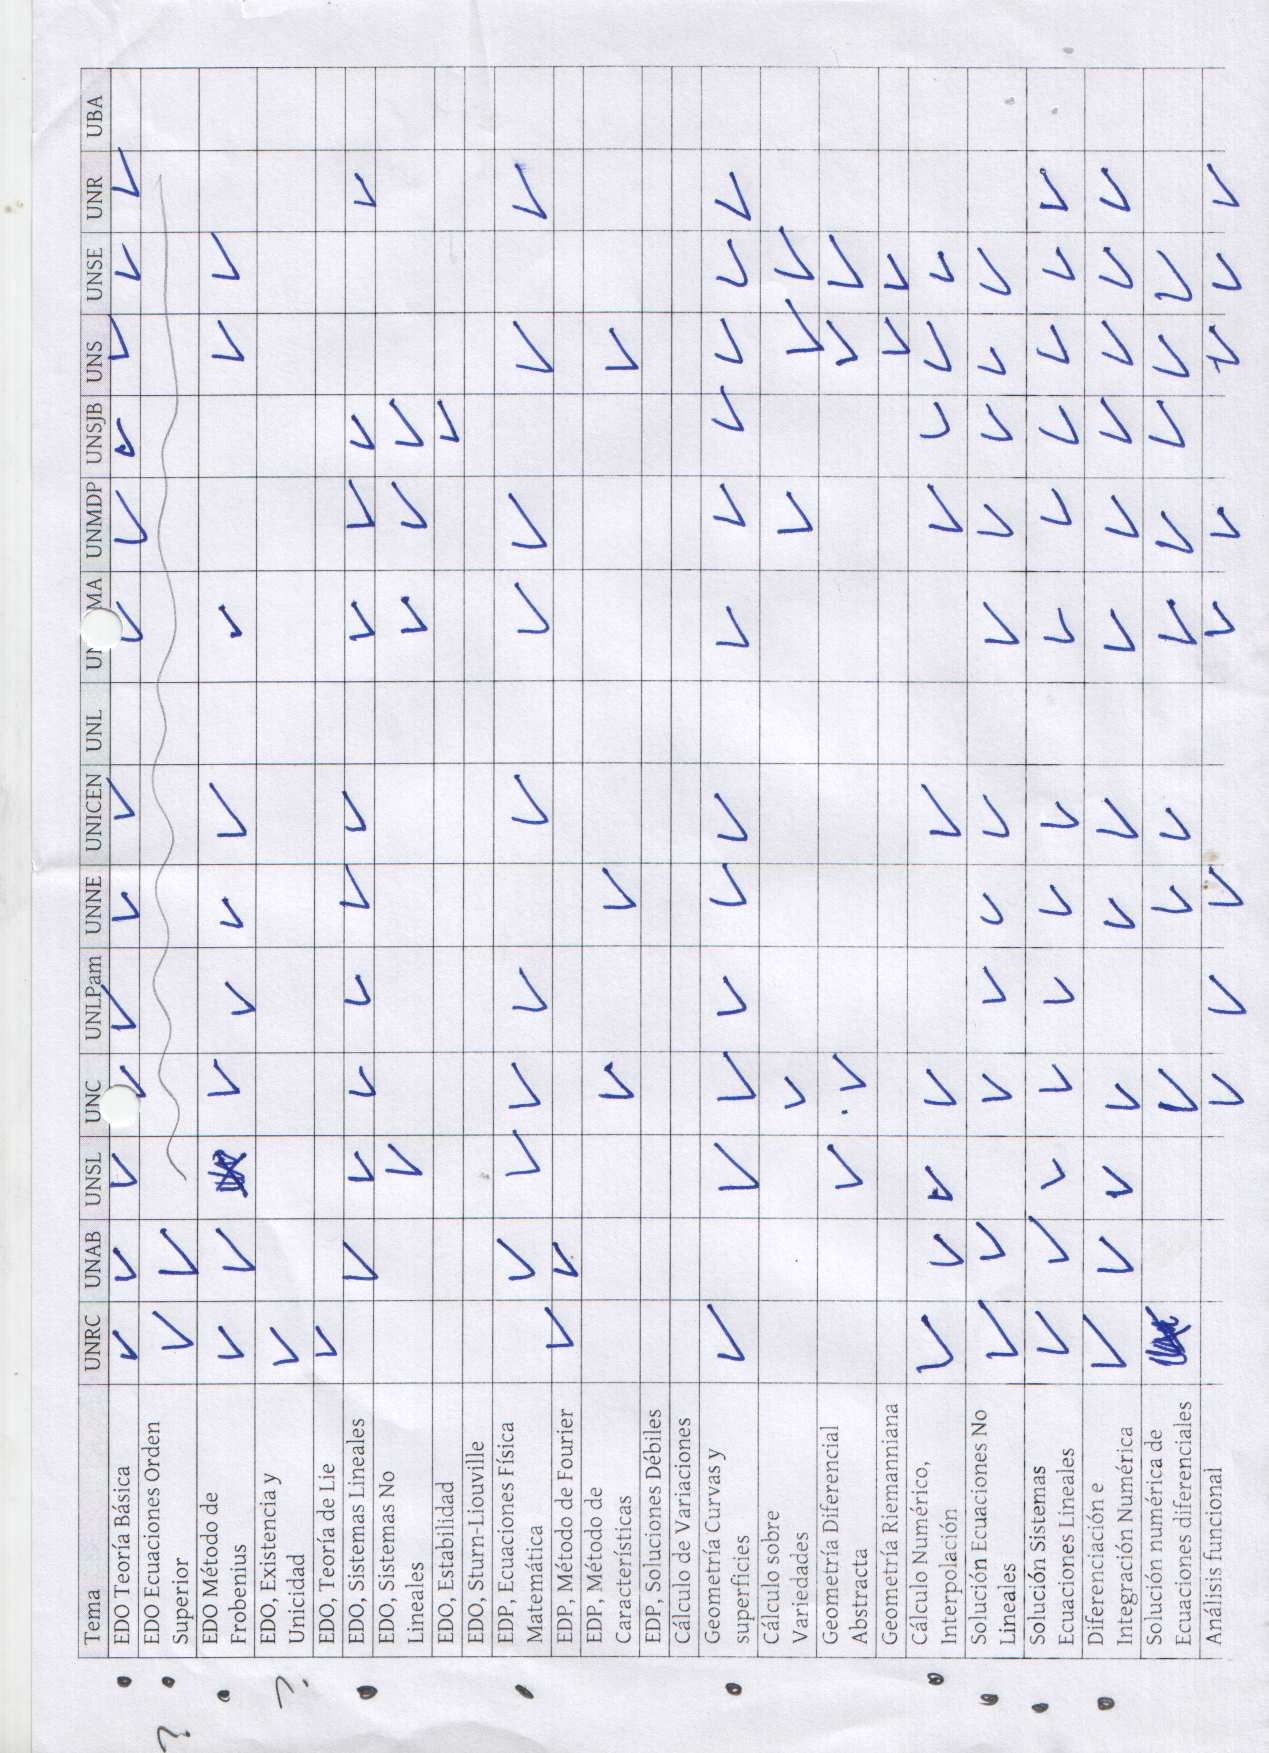
\includegraphics[scale=.3]{01-1.jpg}
\newpage
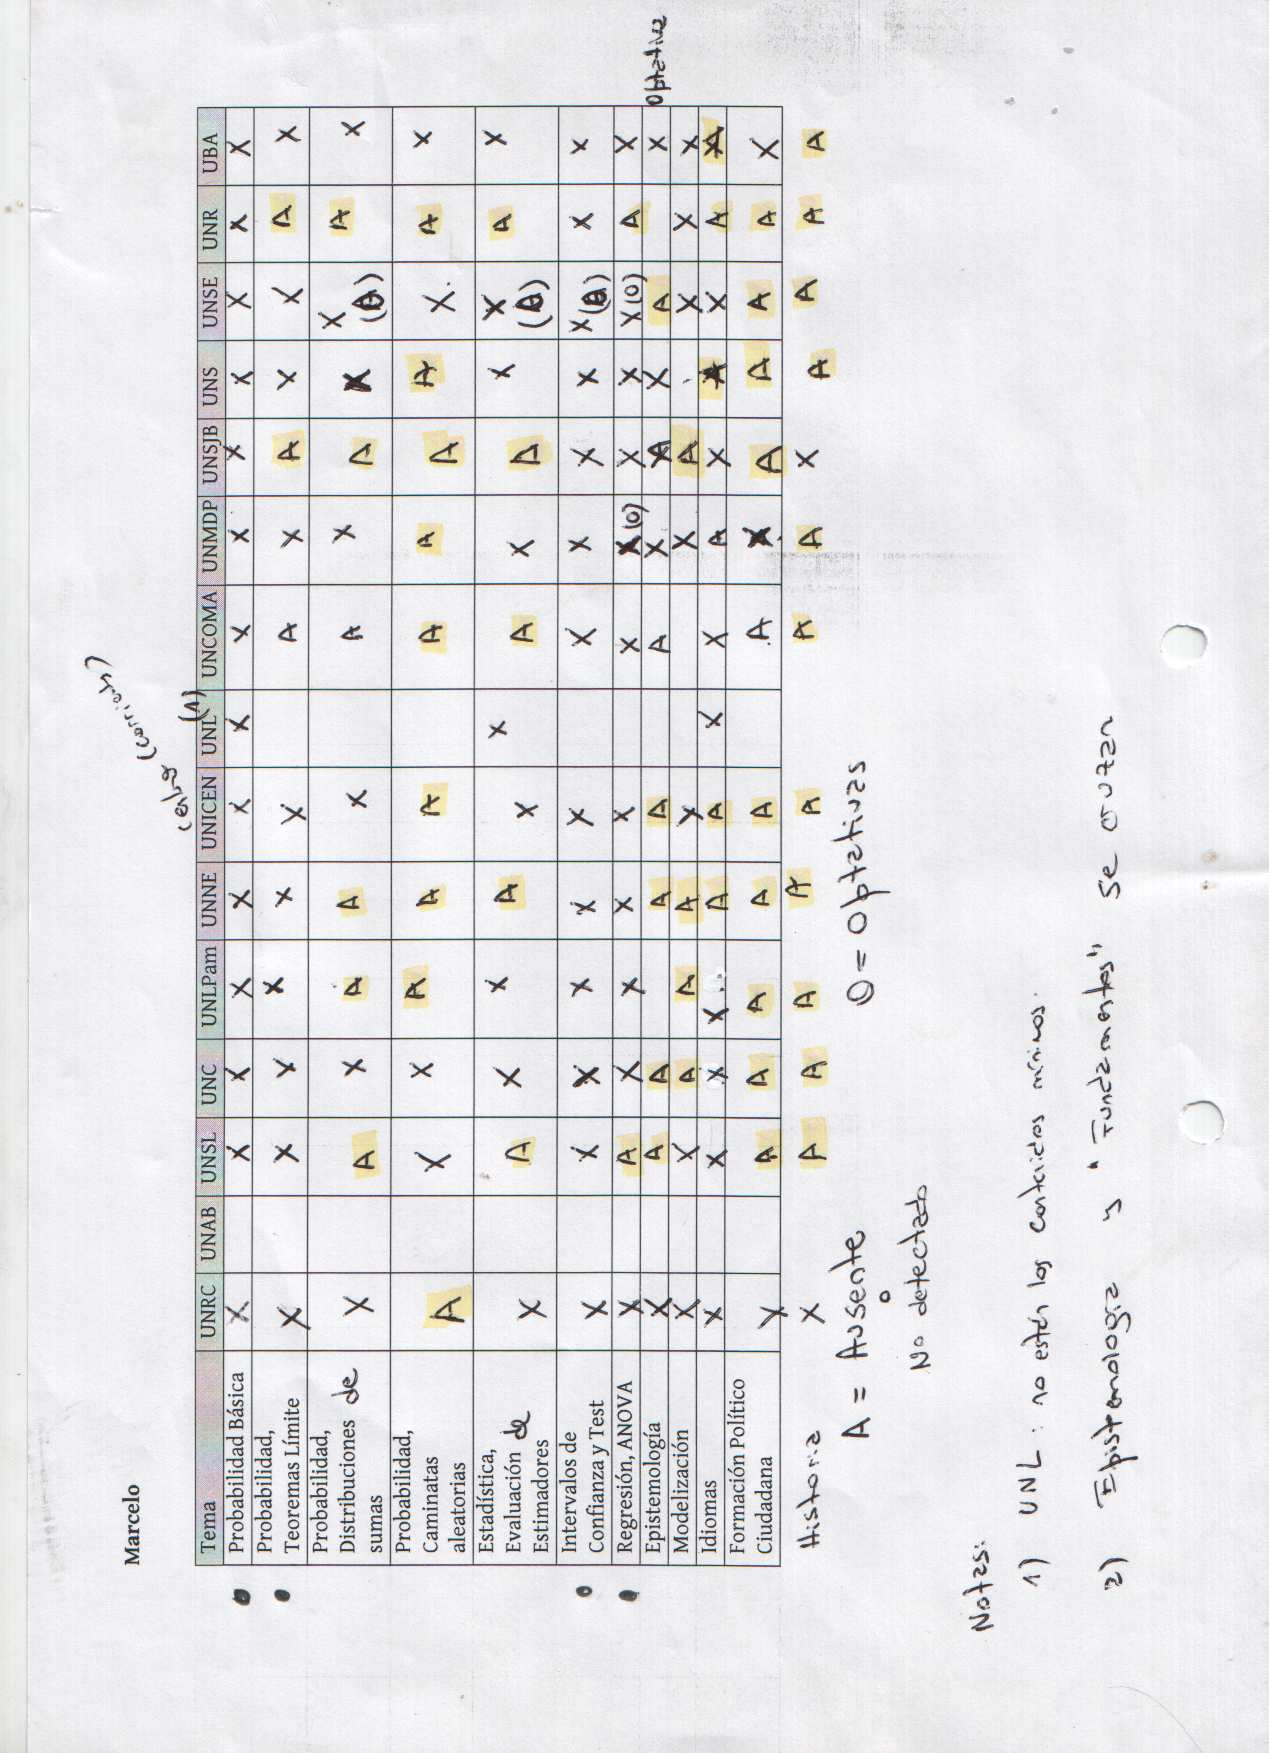
\includegraphics[scale=.3]{01-2.jpg}
\newpage
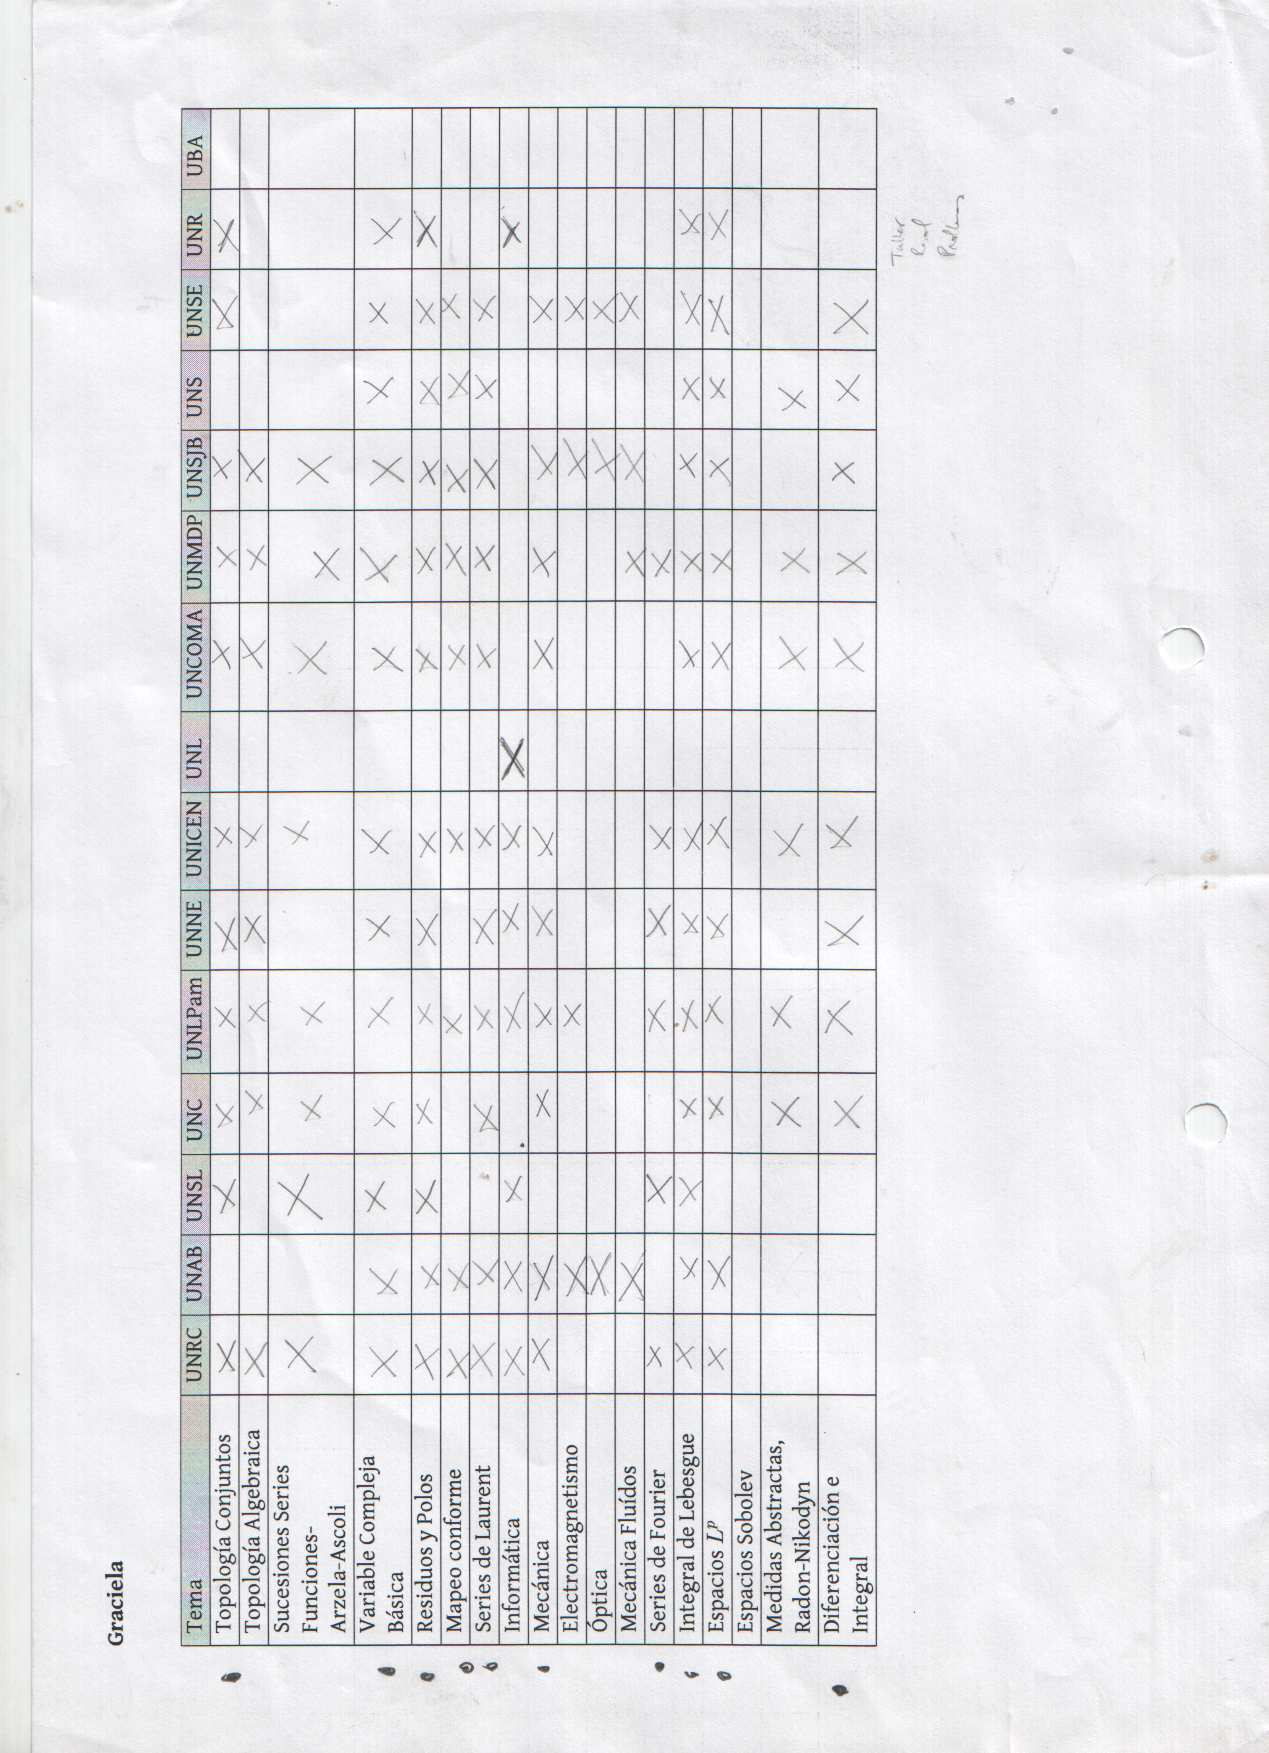
\includegraphics[scale=.3]{01-3.jpg}
\newpage
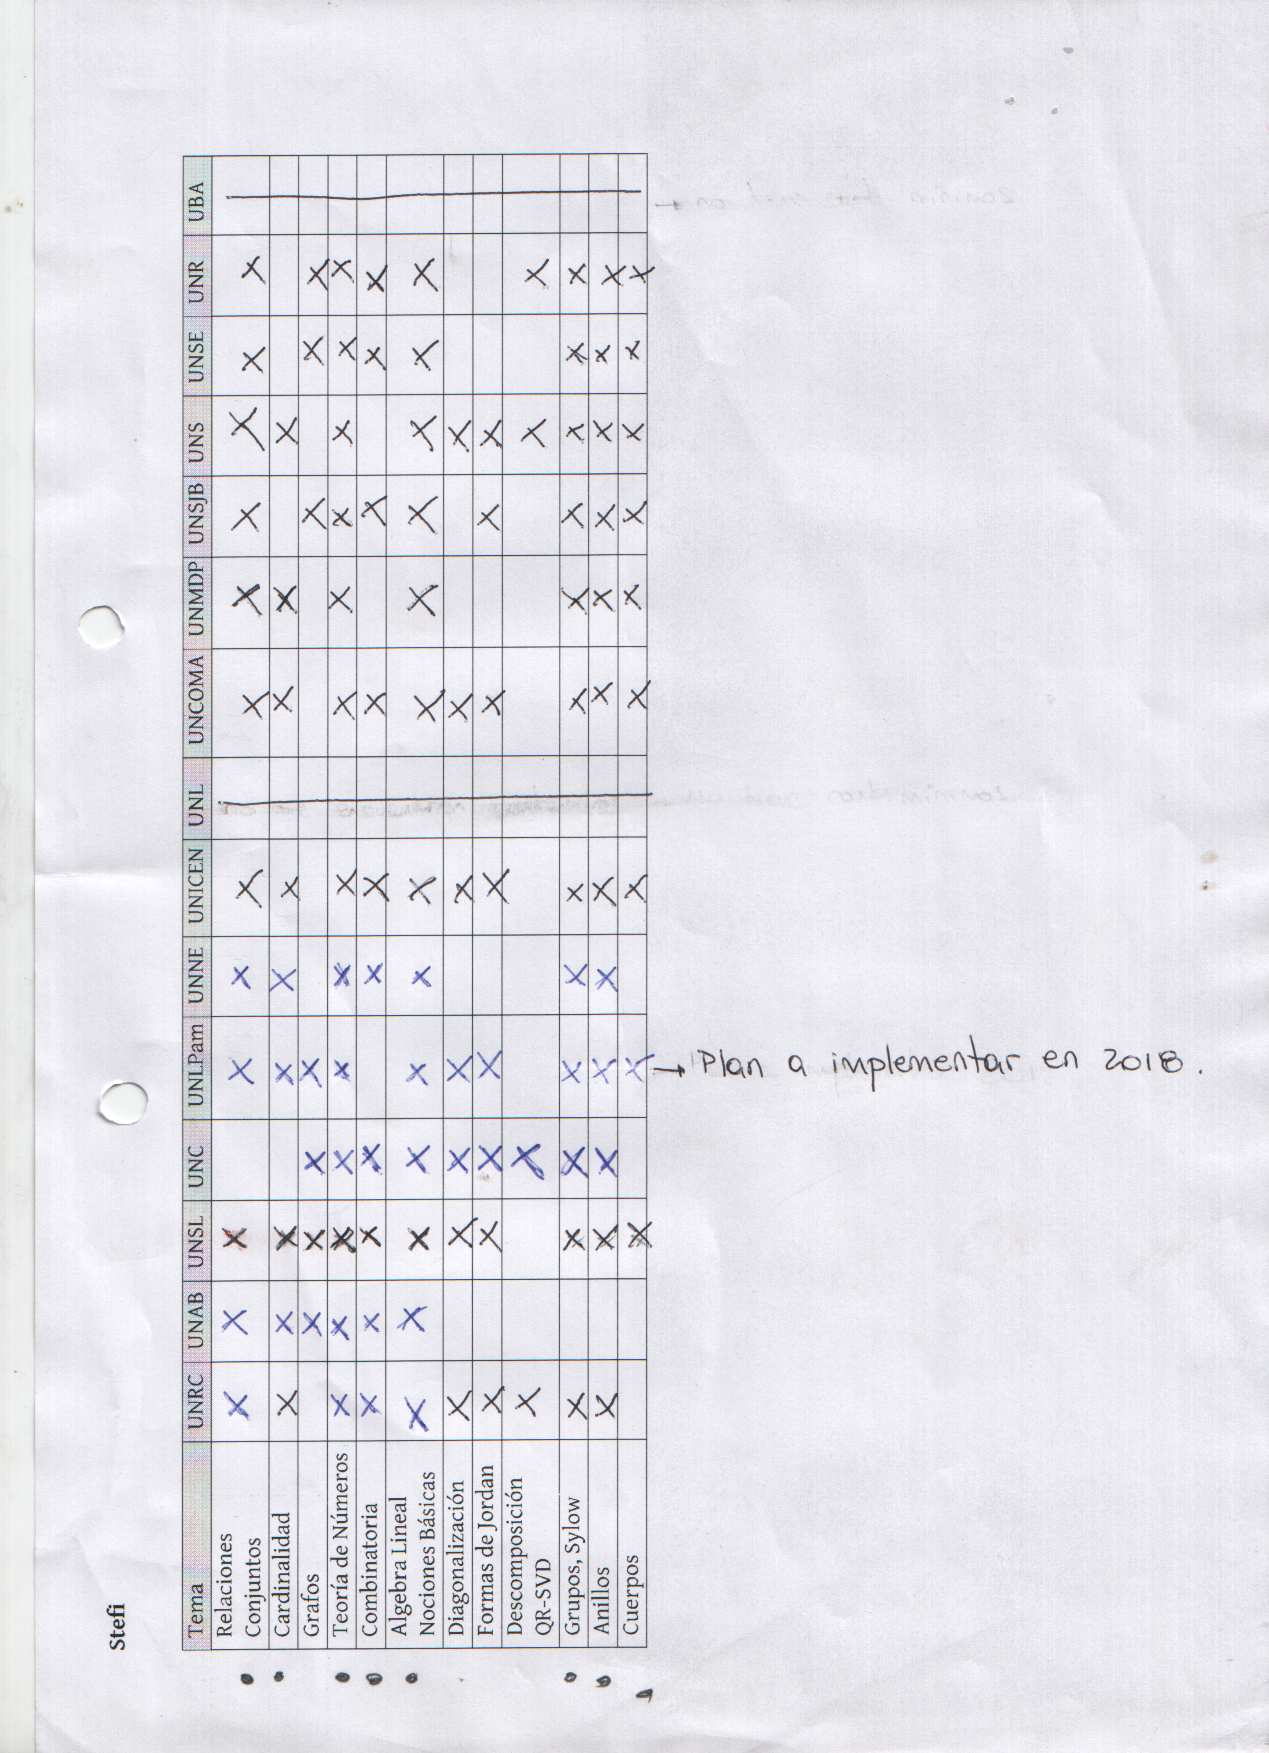
\includegraphics[scale=.3]{01-4.jpg}

\section{Encuesta para docentes}


\paragraph{Pregunta 1}
\begin{center}
 
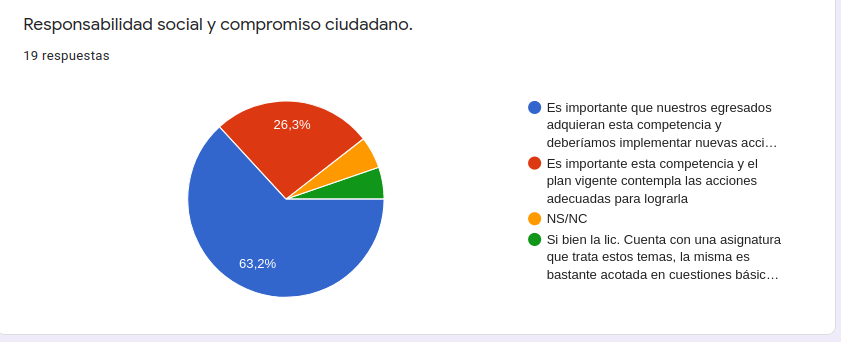
\includegraphics[scale=.9]{doc01.png}
 \end{center}

En caso de haber elegido la primera opción en la pregunta anterior, que acciones puedes sugerir. Entendemos un rango amplio de acciones, como ser: nuevas materias-talleres-seminarios creados con el propósito específico, nuevas metodologías educativas, cambios en la orientación curricular, etc. 8 respuestas

 12 respuestas

 \begin{itemize}
 \item Propongo que se realicen seminarios donde se muestre y enseñe a los alumnos la aplicacion de los contenidos vistos en las asignaturas a la vida diaria. Uno por año a partir del segundo año y que en dichos seminarios se relaciones todas las materias del año anterios.

  \item Una de las acciones a implementar podría ser a través de seminarios que abordeno esta competencia. 
  
 \item Pienso que hay una asignatura destinada a esta temática y esto lo considero suficiente. Sin embargo,  según me han referido algunos estudiantes,   parece ser que el dictado de ella no es del todo riguroso y no estaría logrando el objetivo que se propone. Deberíamos actuar, a través de la Secretaría Académica de la Facultad para corregir la situación.  

 \item  Participar del programa de prácticas socio-comunitarias.

 \item También es importante que los docentes nos manifestemos en torno a problemáticas de la sociedad. Por ejemplo que a través de nuestro órgano colegiado nos expresemos en torno a, por ejemplo, la toma.  
 
 \item Por un lado, la formación en "responsabilidad social y compromiso ciudadano" debería formar parte de la formación específica de un licenciado en Matemática en términos de que dicha formación debería brindar la posibilidad de construir herramientas para formar un pensamiento crítico que permita "interpelar" y/o "cuestionar" la realidad. No obstante, sería muy importante -también- poder implementar espacios específicos de formación al respecto ya que la posibilidad de "conceptualizar" e "intelectualizar" ideas, posicionamientos y aportes teóricos al respecto, aportaría herramientas específicas para el desarrollo de esta competencia.
 
 \item Yo introduciría algún seminario específico, y fomentaría las Prácticas socio Comunitarias o actividades similares. 
 
 \item Considero que debiéramos pensar -en conjunto- en la construcción de espacios curriculares que ayuden a entender el rol de la matemática en la actual sociedad, que se logre valorar el conocimiento matemático como conocimiento NECESARIO  para "entrar" a la sociedad. Si queremos responder a demandas, NO hay DEMANDAS del pueblo, entendiendo el "pueblo"  en sentido amplio, no solo  a los sectores mas populares.  Considero que ésta es una deuda que tenemos y que los currículos en sus clásicos diseños por especialistas deben deconstruir.  Desde este lugar, esto forma parte de la responsabilidad ciudadana que nos cabe por  el privilegio de haber podido acceder a un ámbito público de difusión y construcción de conocimiento científico. 
 
 \item Realizar talleres y seminarios creados con ese propósito
Talleres y/o Seminarios creados con ese propósito

 \item Pueden ser seminarios o talleres cortos con propósitos bien claros y definidos.
 
 \item Mediante algún taller para éste fin especifico que 'obligue' a los estudiantes a involucrarse con las distintas problemáticas sociales.  Esto es para que puedan acercarse  a los sectores más vulnerables desde lo económico, también a personas con capacidades diferentes entre otros. Por que cualquiera sea el ámbito profesional en el que se desarrolle un Lic. en Matemática va a estar en contacto con personas y tienen que poder respetar la diversidad. Ejemplo: siendo docente nos  encontramos con una población de alumnos muy heterogénea y hay que saber respetarlos y comprenderlos.
 
\item a) Incorporar en el currículo contenidos de las sociologías general, de la educación y de la ciencia,  con énfasis en las perspectivas críticas y/o del conflicto b) Ampliar, a nivel departamental, el número de prácticas socio-comunitarias y/o proyectos de extensión 
que articulen currículo con las prácticas sociales de los actores sociales más vulnerables de Río Cuarto c) Promover la participación de los estudiantes en sus en ámbitos institucionales y especialmente en sus organizaciones (centros de estudiantes y agrupaciones)  d) Promover la participación de otras experiencias culturales por fuera del currículo; a modo de ejemplo, "Ciclo de cine por la diversidad" 
La incorporación de prácticas socio-comunitarias en la carrera puede aportar a la reflexión sobre este tema.

\end{itemize}




\paragraph{Pregunta 2}
\begin{center}
 
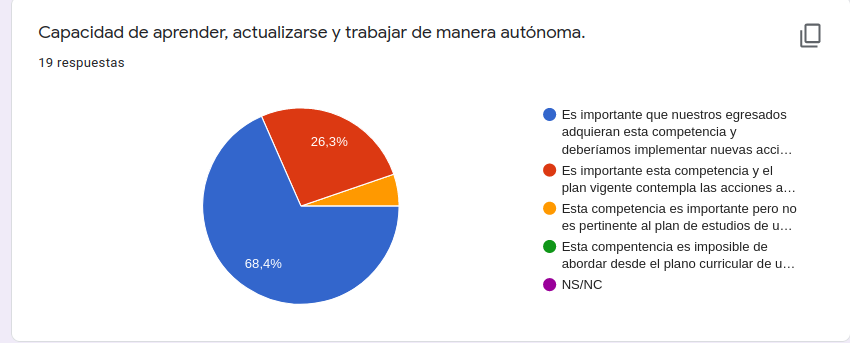
\includegraphics[scale=.9]{doc02.png}
 \end{center}

 En caso de haber elegido la primera opción en la pregunta anterior, que acciones puedes sugerir. Entendemos un rango amplio de acciones, como ser: nuevas materias-talleres-seminarios creados con el propósito específico, nuevas metodologías educativas, cambios en la orientación curricular, etc. 
 
 12 respuestas

 \begin{itemize}
 \item Uso de nuevas metodologías educativas y materiales curriculares que propicien el trabajo autónomo e induzcan al alumno a esta forma de trabajo.
 
\item Creo que a nuestros estudiantes les deberíamos diseñar prácticas donde deban  enfrentar situaciones de manera autónoma. Es mi impresión que el trabajo práctico de las distintas asignaturas se lleva adelante de una manera muy tutelada.  Es probable que esto sea así, porque los docente encontramos que hay un desajuste entre lo que pretendemos enseñar y lo que el alumno está en condiciones de aprender. Como no logramos que resuelvan los problemas que les proponemos, diseñamos actividades donde se realiza una práctica con mucho asesoramiento o ellas, y sus consecuentes exámenes prácticos, consisten de ejercicios donde se implementan métodos y procedimientos.  

\item Sólo modificaría la metodología, incluyendo trabajos para resolver en forma autónoma en algunas asignaturas  

\item Considero esta competencia fundamental y transversal a cada espacio curricular. No existe una metodología para aprender matemática autónomamente que pueda contenerse en un espacio específico.  Lo que considero que nos falta es trabajo colectivo en la institución formadora, donde prime el acto reflexivo en torno a qué matemática enseñar y como pensar en transposiciones que hagan funcional ese conocimiento. 

\item Desde cada asignatura promover el trabajo autónomo, impulsar a la búsqueda de trabajos y lecturas como paper por ejemplo. Se podría dar un pequeño seminario de como indagar los mismos, diferentes revistas científicas etc.

\item Implementar nuevas metodologías en cada asignatura

\item Nueva metodologías, implementar en cada asignatura 

\item Creo que debería destinarse un espacio curricular para debatir las actualizaciones de esta ciencia y otras, tanto entre docentes como estudiantes.

\item Creo que hay docentes que con su metodología de trabajo favorecen a la autonomía de los estudiantes. Pero considero que  no debe ser que esto suceda por las persona en sí que estén como docentes, sino debe ser algo propio de todas las materias desde los primeros años (Ejemplo: metodología de evaluación- Hacer desde los primeros años pequeños trabajos de investigación. No que haya una sola materia que sea un seminario de investigación sino que se incorpore en varias materias)

\item a) Que cada asignatura tenga como lectura real más de un texto de referencia b) Promover la lógica de la investigación en el aula, b) Alentar la participación de lxs estudiantes en proyectos de investigación y ayudantías de segunda c) Alentar tanto la resolución como, y especialmente, el planteo de problemas.

\item Debemos proveer una formación sólida que permita a los egresados  potenciar las líneas de investigación vigentes en el Departamento de Matemática, asimismo poder participar de otros grupos de investigación de la Universidad y  de otras instituciones. Además la capacidad de autonomía permitirá fortalecer las áreas más débiles de nuestro Departamento creando nuevas líneas de investigación. 
Talleres o seminarios en donde se trabaje esta capacidad. Además, creo debe intentarse potenciar esta capacidad en el trabajo diario realizado en cada materia.
\end{itemize}

\paragraph{Pregunta 3}
\begin{center}
 
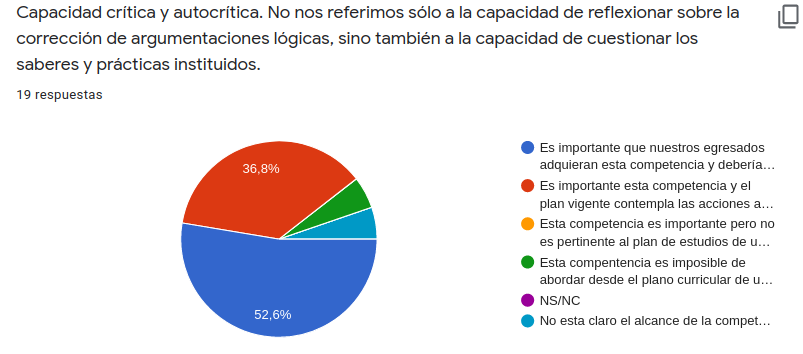
\includegraphics[scale=.9]{doc03.png}
 \end{center}

 
 En caso de haber elegido la primera opción en la pregunta anterior, que acciones puedes sugerir. Entendemos un rango amplio de acciones, como ser: nuevas materias-talleres-seminarios creados con el propósito específico, nuevas metodologías educativas, cambios en la orientación curricular, etc. 
 
 8 respuestas
 
\begin{itemize} 
\item Implementar nuevas metodologías educativas 

\item a) A las observaciones formuladas en la pregunta 1,  agrego "alentar la participación de los estudiantes en la vida política universitaria y de la ciudad" b) la historización de los contenidos de matemática es una perspectiva que necesitamos asumirla de modo transversal a las asignaturas como una forma de desnaturalizar conceptos y formas institucionales c) La participación de nuestrxs estudiantes en programas de intercambios en el país como en América Latina podría favorecer las perspectivas críticas

\item En este caso considero que habría que revisar la metodología usada en general en las clases en pos de lograr en los alumnos la revisión crítica, la reinversión de los contenidos, la búsqueda de relaciones, los fundamentos del por qué de la enseñanza aprendizaje de ciertos contenidos. No olvidemos que quienes estudian la licenciatura también serán docentes en el nivel universitario (y muchos en el nivel medio).

\item Metodologías educativas, en cada asignatura para lograrlo

\item Los docentes deberíamos alentar la crítica y cuestionamiento el saber instituido. Deberíamos cuestionarnos sobre  el sentido del saber que impartimos, su importancia y relación con el resto de la matemática y la ciencia en general.

\item Creo que durante el cursado  de las asignaturas ya existentes se debe favorecer a la autocrítica y esto se debe ver reflejado en la evaluación.

\item Es muy importante la revisión metodología al interior de los espacios curriculares ya que para lograr una capacidad crítica y autocrítica resulta fundamental generar -en los espacios de formación- posibilidades de "reflexión" sobre el hacer matemático.

\item Todo lo que plantee en la anterior pregunta sumando además la necesidad de una revisión de la organización y estructuración de las asignaturas que supere el clásico planteo de secuenciación de contenidos conceptuales, para repensarlas en torno a problemas. O sea organizar los currículos en torno a problemas que permitan una creativa actividad matemática por parte de los alumnos con sus conocimientos disponibles pero que permitan a su vez la emergencia de nuevas proposiciones, definiciones, teoremas que mediante una gestión continua pero reguladora del docente se reconozcan en las clases  como nuevos objetos a ser utilizados. Sin duda este posicionamiento tensiona una clásica organización institucional:   el armado de las materias como Teórico y Prácticos.

\end{itemize}

\paragraph{Pregunta 4}
\begin{center}
 
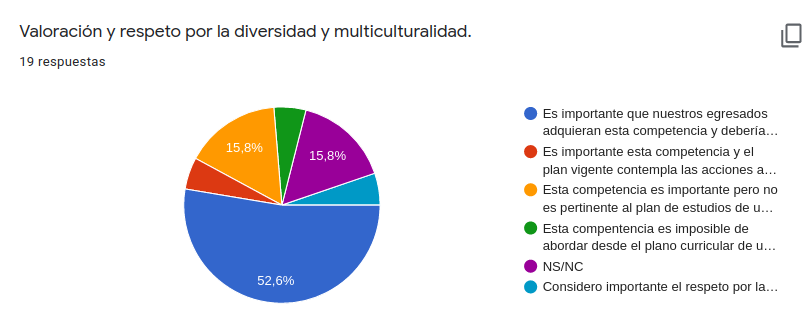
\includegraphics[scale=.9]{doc04.png}
 \end{center}

 
 En caso de haber elegido la primera opción en la pregunta anterior, que acciones puedes sugerir. Entendemos un rango amplio de acciones, como ser: nuevas materias-talleres-seminarios creados con el propósito específico, nuevas metodologías educativas, cambios en la orientación curricular, etc. 
 
 8 respuestas

 \begin{itemize}
\item  Realizar talleres creados con el propósito específico

\item a) Que nuestro departamento incorpore en su lenguaje institucional las normativas ya sancionadas a nivel nacional y también a nivel local, UNRC. A modo de ejemplo, que en nuestra web la normativa de identidad de género y el reglamento de violencia de género queden explicitados b) Promover la participación de docentes, no-docentes y estudiantes en espacios educativos y culturales que favorezcan la diversidad en sus diferentes dimensiones c) Promover la generación de proyectos de extensión y/o prácticas socio-comunitarias que incorporen la problemática  c) La participación de nuestrxs estudiantes en programas de intercambios en el país como en América Latina podría favorecer las perspectivas críticas.

\item Talleres creados con el propósito específico

\item Es oportuno destacar que dentro del departamento se realizan acciones en la dirección de la inclusión, por ejemplo elaborando material didáctico para no videntes.  Sin llegar a crear nuevas materias sobre esta temática hay algunas otras acciones que si bien no forman parte de un currículo formal creo que aportarían en la dirección señalada. Por ejemplo, que los docentes nos manifestemos en torno a problemáticas de genero y diversidad cultural, que nuestro órgano colegiado, el consejo departamental, se manifieste avalando acciones de la comunidad en defensa de la diversidad sexual y cultural (marcha de la gorra y la diversidad, etc). Hay que valorar el carácter pedagógico de estas acciones. 

\item Es un poco lo que conteste en la primer pregunta. Debe haber talleres específicos  que hagan que los estudiantes se vinculen con 'diferentes'  grupos de personas.

\item Quizás resulte necesario un abordaje específico para avanzar -en primer lugar- en la "comprensión" de lo diverso y multicultural para -luego- pensar la posibilidad de una formación que no sólo contemple sino que se base en el respecto y valoración de la diversidad y multiculturalidad.

\item En este caso propondria que haya una o dos asignaturas para capacitar y darle estrategias a nuestros alumnos para aceptar, respetar y comprender la heterogeneidad cultural actual.

\item Análogamente a  respuestas anteriores considero que estos valores necesarios para pensar una sociedad diferente más igualitaria y menos fóbica deberían fomentarse transversalmente en todo el desarrollo del programa de estudios. Quizás un trabajo colectivo en tanto institución formadora de profesionales del conocimiento científico, nos ayudaría a reflexionar sobre qué significa "ser docente" en el ámbito universitario, y además en una Universidad pública. Que sin duda supera toda mirada simplista que valore solo la especialidad matemática
\end{itemize}
 \paragraph{Pregunta 5}
\begin{center}
 
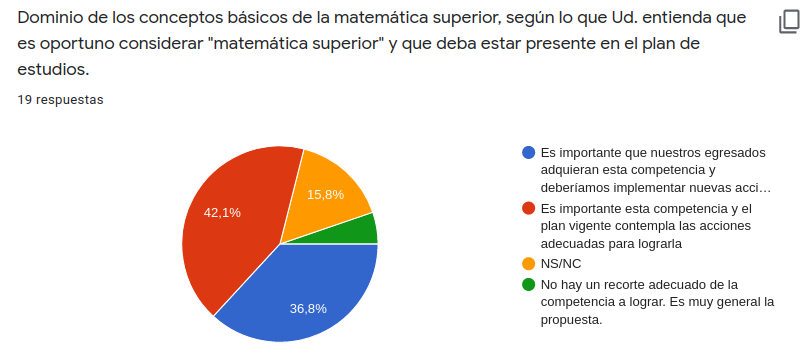
\includegraphics[scale=.9]{doc05.png}
 \end{center}
 En caso de haber elegido la primera opción en la pregunta anterior, que contenidos debería contemplar el nuevo plan de estudios que no contempla el actual. 
 
 7 respuestas
 \begin{itemize}
 \item Problemas de grafos (como conectividad y coloreo), cardinalidad (teorema de Schoreder-Cantor), teorema de Radom-Nykodim y su vinculación con esperanzas condicionales, cadenas de markov y nociones generales de procesos estocásticos (martingalas),  transformada de Fourier y teormas de inversión, nociones de aprendizaje de máquinas y aprendizaje estadístico (machine y statistical learning), funciones monótonas y de variación acotada.
 
\item Las carrera de 4 años no permite contemplar los conceptos básicos de la matemática superior. Faltan contenidos en álgebra, análisis funcional, ecuaciones en derivadas parciales, etc.

\item El nuevo plan de estudios debería contemplar como materias obligatorias: Ecuaciones en Derivadas Parciales y Análisis Funcional

\item Me parece que el nuevo plan debería contemplar más contenidos de estadística, mapeo conforme, ecuaciones en derivadas parciales, series de Fourier, Teoría de Optimización y quizás algunas otras que me estoy olvidando.

\item Considero que es bastante completo el plan.

\item Desde mi punto de vista, agregaría contenidos básicos de lógica en primer año. Ejemplo: Si bien se puede entender intuitivamente la negación de la definición de la existencia de un límite, no puede ser que alguien que estudie matemática no pueda negar una proposición que tenga conectores y cuantores lógicos, entre otras cosas (esto como base para todas las materias que se dictan).

\item Tal vez falten algunos contenidos básicos de geometría. 
Con respecto a contenidos de matemática superior, considero necesario que se dicten contenidos de análisis funcional.

\item Álgebra: Más temas acerca de Polinomios y Ecuaciones Algebraicas. Teoría de Módulos, Grupos finitos, Extensiones de Grupo y de Cuerpo. Matemática Discreta: Combinatoria, Teoría de Grafos,  Análisis Funcional y Ecuaciones Diferenciales en Derivadas Parciales.

\item Específicamente considero que en la denominada Matemática superior debería incluirse un espacio curricular sobre Epistemología de la Matemática.
 \end{itemize}
 
 
 
  \paragraph{Pregunta 6}
\begin{center}
 
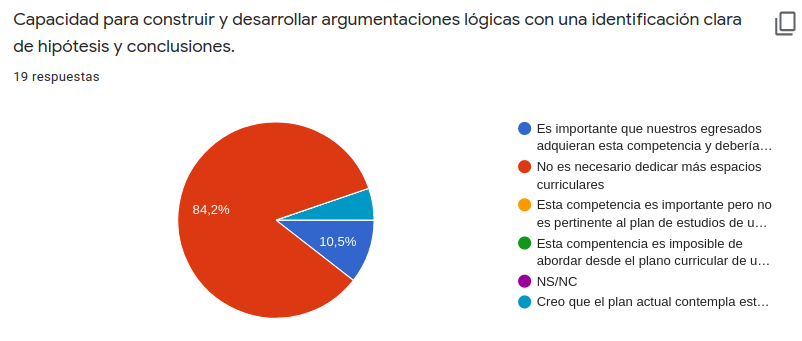
\includegraphics[scale=.9]{doc06.png}
 \end{center}
 En caso de haber elegido la primera opción en la pregunta anterior, que acciones puedes sugerir. Entendemos un rango amplio de acciones, como ser: nuevas materias-talleres-seminarios creados con el propósito específico, nuevas metodologías educativas, cambios en la orientación curricular, etc. 
 
 1 respuesta

  \begin{itemize}
  \item Como dije en la pregunta anterior se necesitan conocimientos de lógica, y que estos conocimientos se afiancen en las distintas asignaturas. 
  \end{itemize}
 
  
  \paragraph{Pregunta 7}
\begin{center}
 
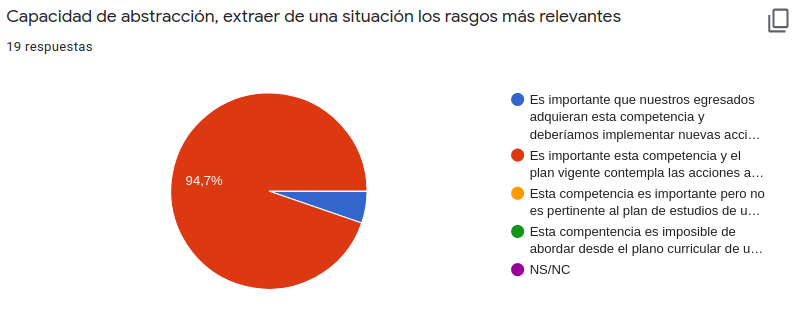
\includegraphics[scale=.9]{doc07.png}
 \end{center}
 En caso de haber elegido la primera opción en la pregunta anterior, que acciones puedes sugerir. Entendemos un rango amplio de acciones, como ser: nuevas materias-talleres-seminarios creados con el propósito específico, nuevas metodologías educativas, cambios en la orientación curricular, etc. 
 
 1 respuesta

 
   \begin{itemize} 
   \item Considera que esto se logra con la metodología de enseñanza.
  \end{itemize}
  
    
  \paragraph{Pregunta 8}
\begin{center}
 
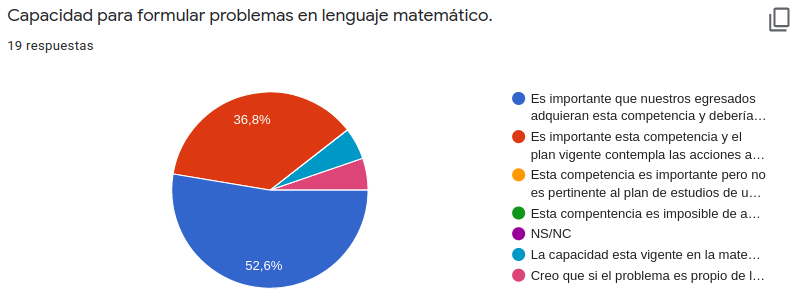
\includegraphics[scale=.9]{doc08.png}
 \end{center}
  En caso de haber elegido la primera opción en la pregunta anterior, que acciones puedes sugerir. Entendemos un rango amplio de acciones, como ser: nuevas materias-talleres-seminarios creados con el propósito específico, nuevas metodologías educativas, cambios en la orientación curricular, etc. 
  
  9 respuestas
  
  
   \begin{itemize} 
\item Implementar nuevas metodologías educativas que trabaja con problemas a resolver en cada asignatura

\item El plan debería contemplar el cursado de asignaturas de otras disciplinas junto a estudiantes de otras carreras. A modo de ejemplo, física y  algorítimica deberían cursarse junto a lxs estudiantes de física y computación.

\item Se deberían trabajar con más modelos matemáticos al interior de las asignaturas. Considero que se trabaja en la asignatura modelos matemáticos y en muy pocas otras en unidades temáticas específicas. 

\item Nuevas metodologías educativas, para implementar en cada asignatura

\item Habría que agregar talleres en el cual, por ejemplo, se formulen en lenguaje matemático problemas provenientes de otras áreas

\item Entiendo que se refiere a la capacidad de modelar, y tanto docentes como estudiantes tendríamos que capacitarnos más en esto. Especialmente en matemática aplicada.

\item Entiendo que esta competencia requiere que el estudiante aborde otros objetos de estudio aparte de los matemáticos, de modo que pueda vislumbrar una estructura matemática subyacente en ellos y transmitirla en el lenguaje propio de la matemática. Hay pocas materias donde pongamos al estudiante en esta situación.
 
\item Yo modificaría la metodología de enseñanza, introduciendo en algunas asignaturas problemas de otras áreas del conocimiento que puedan formularse en lenguaje matemático.
  
\end{itemize}




    
  \paragraph{Pregunta 9}
\begin{center}
 
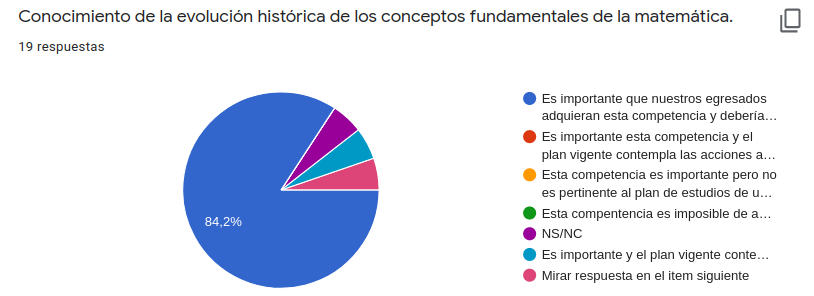
\includegraphics[scale=.9]{doc09.png}
 \end{center}

 En caso de haber elegido la primera opción en la pregunta anterior, que acciones puedes sugerir. Entendemos un rango amplio de acciones, como ser: nuevas materias-talleres-seminarios creados con el propósito específico, nuevas metodologías educativas, cambios en la orientación curricular, etc. 
 
 16 respuestas

\begin{itemize}
 \item Implementar talleres que contemplen este aspecto. 

 \item implementar nuevas materias con los contenidos pertinentes

 \item a) Epistemología e historia de la matemática son disciplinas que deben transversalizar el currículo b) Debe sostenerse tanto historia como epistemología como una opción del cuerpo de asignaturas optativas.

 \item Puede ser la creación de un espacio propio (asignatura, taller, seminario) como historia y epistemología de las matemáticas junto a la incorporación al interior de cada asignatura de cuestiones generales que hacen a esos contenidos. 

 \item Taller o Seminario

 \item Tendría que haber un espacio para estudiar historia y fundamentos de la matemática. Creo que actualmente depende del docente la incorporación de estos contenidos en cada materia.

 \item Se debería incorporar en el transcurso del dictado de cada una de las asignaturas.
nuevas materias como historia de la matemática serían oportunas

\item Sería oportuno que en tantas materias como se pueda se transmita la idea que la matemática no es un estructura monolítica e inalterable, sino que es un objeto histórico que transcurre en el tiempo y evoluciona no sólo de manera acumulativa, por ejemplo que tiene eventos disruptivos. Es menester que contextualicemos históricamente los conceptos que pretendemos enseñar.  

\item No creo que sea necesario alguna materia especifica sino que se trate (en algunas materias) de dar los contenidos tratando de mostrarles a los alumnos cual fue toda la construcción histórica hasta llegar al concepto o teorema, etc que tiene relevancia en la actualidad.

\item Incorporación de una  nueva materia

\item Debería formar parte del trabajo en los espacios curriculares.

\item Materias donde se aborde la filosofia e historia de la matematica.

\item Contextualizar las Matemáticas por medio de su historia es un esfuerzo que se debería al menos intentar ya sea desde las asignaturas ya vigentes o bien dedicando un nuevo espacio curricular  a la Historia de las Matemáticas ya que ésta puede proporcionarle una visión verdaderamente humana a las matemáticas que muchas veces es percibida como una ciencia fría e infalible.  
La Historia de la Matemáticas puede representar un valioso recurso en la construcción de estrategias necesarias para formar estudiantes reflexivos y críticos (que preguntan el qué, el cómo, el dónde y el por qué). De esta manera se pueden conocer los desacuerdos, los errores, los problemas y las necesidades que se encuentran tras la historia de cada concepto matemático,  proporcionándole al estudiante la posibilidad de dudar y generar debates interesantes. Quizás una manera de implementar este espacio sea mediante un seminario donde estudiantes y docentes puedan exponer/debatir la correlación de un concepto matemático con su respectiva evolución histórica.  

\item No estoy pensando en una historia de los conocimientos matemáticos. justamente conocer la "razón de ser" de objetos  que estructuran y otorgan el sentido esencialmente modelizador de la matemática significa estudiar la epistemología de los saberes.  Ahora bien, ¿qué saberes?,¿que desarrollo y hasta donde? son interrogantes que nuevamente, considero, deben ser discutidos colectivamente y en relación con otras instituciones. 

\item Incorporar alguna asignatura (o parte de una asignatura)
 
 
\end{itemize}


  \paragraph{Pregunta 10}
\begin{center}
 
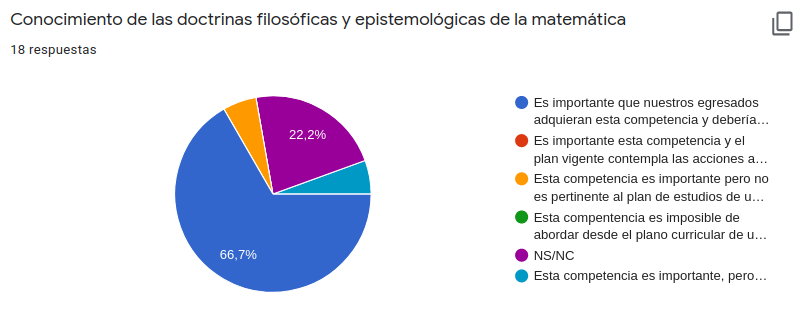
\includegraphics[scale=.9]{doc10.png}
 \end{center}
En caso de haber elegido la primera opción en la pregunta anterior, que acciones puedes sugerir. Entendemos un rango amplio de acciones, como ser: nuevas materias-talleres-seminarios creados con el propósito específico, nuevas metodologías educativas, cambios en la orientación curricular, etc.

13 respuestas
\begin{itemize}
 \item Implementar talleres que aborden esta competencia y junto con la evolución histórica.
 
\item Implementar nuevas materias que contemplen contenidos relacionados con esta competencia junto con la evolución histórica de los conocimientos matemáticos

\item Epistemología e historia de la matemática son disciplinas que deben transversalizar el currículo

\item Es muy importante estas discusiones y aprendizajes, como ya lo mencioné con anterioridad.

\item Nueva materia

\item Se podría incluir una asignatura en donde se estudie historia y epistemologia ya que el plan curricular actual no contempla estos items. 

\item espacios como epistemología o filosofía serían necesarias

\item Incorporación de una  nueva materia

\item Debería formar parte del trabajo en los espacios curriculares pero sería muy importante la posibilidad de un espacio específico para que las doctrinas filosóficas y epistemológicas de la matemática se constituyan en "objetos de estudio".

\item Igual a la anterios. Matetias donde se pueda tener conocimiento de esta area.

\item Idem a la respuesta anterior. 

\item Creo que respuestas anteriores validan esta elección.
Incorporar alguna asignatura (o parte de una asignatura)
\end{itemize}


  \paragraph{Pregunta 11}
\begin{center}
 
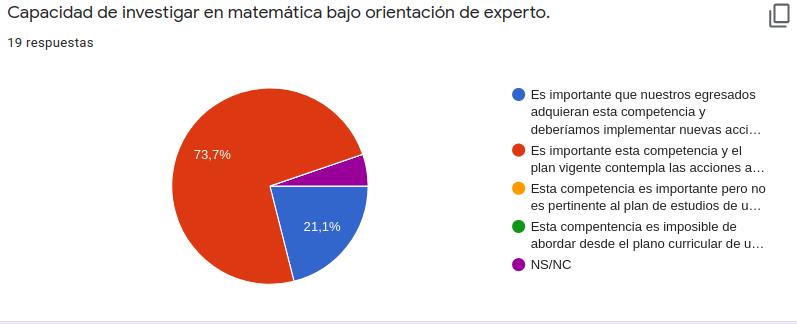
\includegraphics[scale=.9]{doc11.png}
 \end{center}

 En caso de haber elegido la primera opción en la pregunta anterior, que acciones puedes sugerir. Entendemos un rango amplio de acciones, como ser: nuevas materias-talleres-seminarios creados con el propósito específico, nuevas metodologías educativas, cambios en la orientación curricular, etc. 
 
 4 respuestas
 
 \begin{itemize}
  \item Incorporar seminarios relativos a este tema e implementar estas capacidades dentro de cada asignatura
\item Nueva materia

\item Talleres o seminarios en donde se trabaje esta capacidad
\item Implementar talleres optativos para que los alumnos trabajen en un lineamiento que les interese desde segundo año. Y ademas para mostrarle e interiorirarlos en las investigaciones existentes en nuestro departamento pero desde adentro, para ello deben participar.
 \end{itemize}


 
  \paragraph{Pregunta 12}
\begin{center}
 
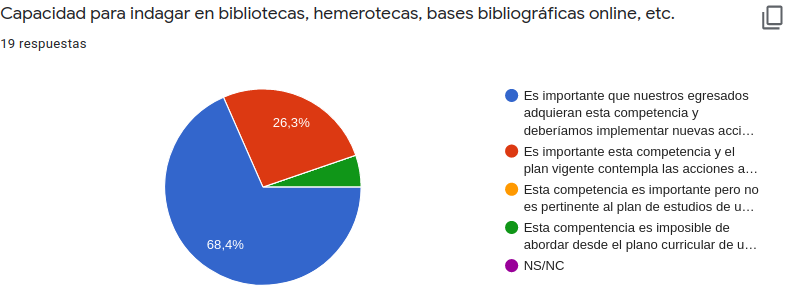
\includegraphics[scale=.9]{doc12.png}
 \end{center}
 
  
  \paragraph{Pregunta 13}
\begin{center}
 
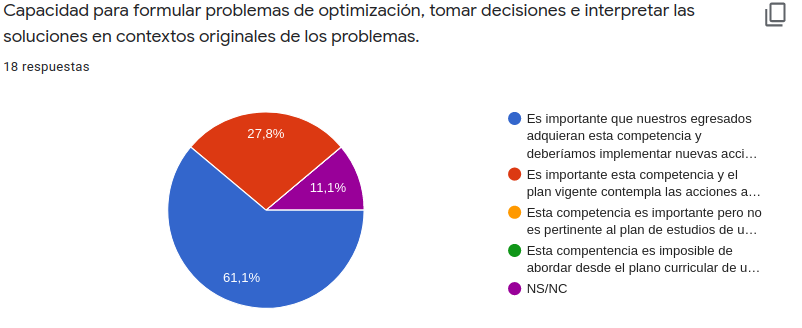
\includegraphics[scale=.9]{doc13.png}
 \end{center}
 
 En caso de haber elegido la primera opción en la pregunta anterior, que acciones puedes sugerir. Entendemos un rango amplio de acciones, como ser: nuevas materias-talleres-seminarios creados con el propósito específico, nuevas metodologías educativas, cambios en la orientación curricular, etc.
 
 11 respuestas

 \begin{itemize}
  \item Incorporar en algunas asignaturas problemas aplicados 
 \item Incorporar en espacios curriculares pertinentes optimización e interpretar en contextos reales 

  \item En cada espacio curricular deberíamos trabajar la capacidad de interpretar y comunicar resultados en contexto del problema.
 \item Debería haber un espacio curricular con aplicaciones concretas de la matemática.
 \item Agregar contenidos de teoría de optimización. 
 \item Es fundamental. No debe ser algo propio de una materia, sino de todas. No es que se deban cambiar los contenidos de las materias sino, como ya dije, el tipo de problemas que se le presenta al alumno.

 \item Nuevas materias y/o trabajar con este tipo de problemas en las materias que ya tenemos.

  \item Quizás sea necesario revisar el tipo de planteo desde los espacios curriculares.

   \item Propongo que se den asignaturas mas aplicadas a la informatica.

    \item Se puede pensar en un espacio tipo el taller de resolución de problemas que actualmente es una asignatura pero donde se resuelvan problemas de Optimización con el uso de entornos computacionales. 
 \item  Incluiría  el tema  optimización como parte de alguna asignatura (nueva) 
 \end{itemize}

   \paragraph{Pregunta 14}
\begin{center}
 
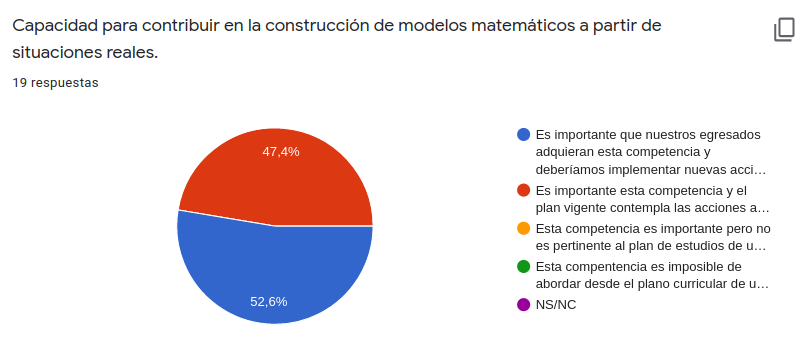
\includegraphics[scale=.9]{doc14.png}
 \end{center}
 
 En caso de haber elegido la primera opción en la pregunta anterior, que acciones puedes sugerir. Entendemos un rango amplio de acciones, como ser: nuevas materias-talleres-seminarios creados con el propósito específico, nuevas metodologías educativas, cambios en la orientación curricular, etc. 
 
 10 respuestas
 
 \begin{itemize}
 
 
\item Cambio en la orientación curricular. 
\item a) Alentar a lxs estudiantes en actividades transdisciplinarias en el marco de la su  participación en proyectos de investigación b) Los proyectos de extensión y las prácticas socio-comunitarias son instancias importantes a los fines de potenciar dichas capacidades

\item Aunque deberían abocarse a ello también  en otros espacios.

\item Abordarlo desde cada asignatura.

\item Es fundamental que los alumnos aprendan a modelar matemáticamente diferentes tipos de problemas (creo que es la principal debilidad que tiene nuestra licenciatura). No se como se logra, calculo que desde el tipo de problemas que se le presentan a los alumnos, la metodología de trabajo. Tiene que ser algo común de todas las asignaturas desde en comienzo de la carrera no que sólo haya una materia en el último año que sea modelos matemáticos por que es muy difícil que allí se  logre lo que no se hizo en los años anteriores.

\item Nuevas materias y/o trabajar con este tipo de problemas en las materias que ya tenemos.

\item Sería muy importante que este trabajo forme parte del "hacer" al interior de los espacios curriculares.

\item Talleres y seminarios de los trabajos de investigacion del dpto pero que los alumnos participen se involucren y aprendan.

\item Idem a la respuesta anterior. Aunque hay una asignatura con este objetivo quizás pueda fortalecerse con otro espacio dedicado a resolver problemas concretos regionales/ nacionales u otros del mundo real. 

\item Considero que es necesario contar con algún espacio curricular nuevo para fortalecer esta capacidad  


 
 \end{itemize}
   \paragraph{Pregunta 15}
\begin{center}
 
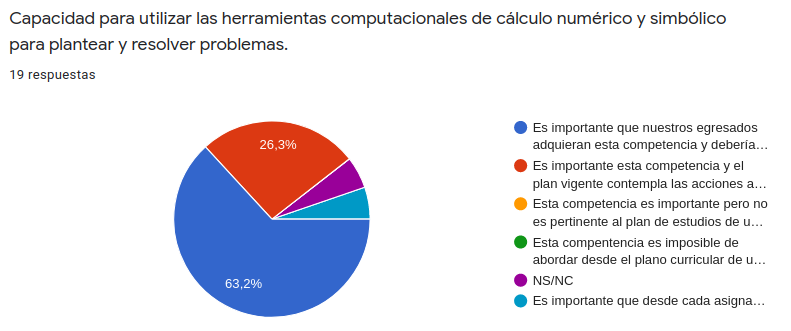
\includegraphics[scale=.9]{doc15.png}
 \end{center}
 

 En caso de haber elegido la primera opción en la pregunta anterior, que acciones puedes sugerir. Entendemos un rango amplio de acciones, como ser: nuevas materias-talleres-seminarios creados con el propósito específico, nuevas metodologías educativas, cambios en la orientación curricular, etc. 
 
 11 respuestas

 \begin{itemize}
  \item a) Algorítimica y estructuras de datos deberían estar presentes en una asignatura en vistas de un aprendizaje de programación independiente de los lenguajes específicos y b) La programación y los algoritmos deben transversalizar el currículo
\item Necesitamos más programación en el plan de estudios

\item Se deberían implementar más espacios curriculares relacionados  a la programación y uso de herramientas computacionales.
\item más espacios de formación en el campo numérico computacional
\item Hay que fortalecer la formación en el área de la informática e integrar la informática en muchas materias. 
\item Es importante que cada vez se implementen más, en las asignaturas que sea posible, el uso de herramientas computacionales. Es importante que haya una materia básica en primer año, pero después en las distintas materias tienen que crear espacios en lo que se aplique lo aprendido en taller de informática o que se trabajen con diferentes software. (Por lo menos con algunos contenidos).
\item Que se mediante el uso de estas herramientas que se pueda llegar a alguna conjetura para luego demostrarla formalmente.
Nuevas materias y/o trabajar con este tipo de problemas en las materias que ya tenemos.
\item Más allá de los espacios específicos, sería importante que se incorpore como parte del trabajo matemático, pudiendo "reflexionar" sobre los alcances, limitaciones y/o potencialidades de las herramientas.
\item Esta capacidad podría fortalecerse con la incorporación de  entornos computacionales (sistemas de cálculo simbólico, software de visualización, paquetes estadísticos, etc ) en los cursos de los primeros años, de tal forma que el estudiante pueda adquirir una experiencia que le permita utilizar esta herramienta en la exploración de conceptos y la resolución de problemas en los cursos posteriores de la carrera o incluso después de que haya egresado. 
\item Considero necesario la construcción de estos espacios curriculares para los cuales además, en este ámbito  hay DEMANDAS. O sea las condiciones para su inclusión están claramente dadas. \item Sólo hay que discutir con los especialistas su estructura curricular en función del perfil que definimos para nuestros egresados.
\item Incluiría actividades que fortalezcan esta capacidad en varias asignaturas de la curricula. 
 
 \end{itemize}
 
 
    \paragraph{Pregunta 16}
\begin{center}
 
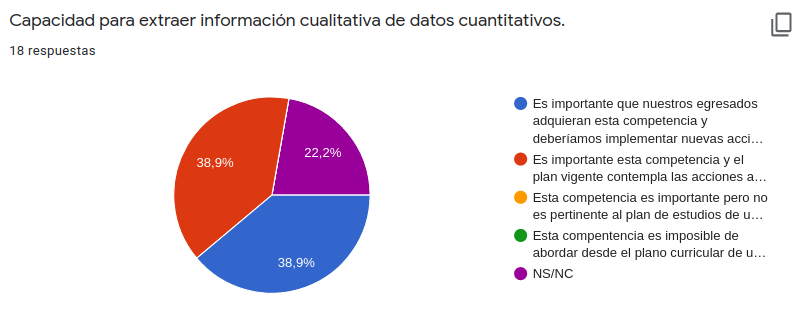
\includegraphics[scale=.9]{doc16.png}
 \end{center}
 

 En caso de haber elegido la primera opción en la pregunta anterior, que acciones puedes sugerir. Entendemos un rango amplio de acciones, como ser: nuevas materias-talleres-seminarios creados con el propósito específico, nuevas metodologías educativas, cambios en la orientación curricular, etc.
 
 7 respuestas
 
 \begin{itemize}
  \item Actualmente se contemplan las acciones para lograr estas capacidades en Estadística y debería implementarse en otros espacios curriculares

  \item Es muy importante, considero que es una falencia grande de nuestros planes. Es necesario un nuevo espacio curricular para trabajarlo o repensar las asignaturas que pueden estar ligadas a ello (probabilidad, estadística, inferencia estadística)
  
\item Actualmente se contemplan acciones en Estadística y deberían incorporarse a otros espacios curriculares existentes.
\item Esta pregunta está ligada a que puedan interpretar soluciones. Nuevamente con el tipo de problemas que se le presenten se va a favorecer esto. 

\item Incorporación de una  nueva materia
\item Revisar y/o fortalecer el trabajo al interior de los espacios curriculares.
\item Idem a la anterior. Sólo refuerzo que el marco de referencia institucional debe ser el perfil del egresado. Esto Sí considero que es necesario discutirlo como un problema de TODOS. Un verdadero problema institucional
 
 \end{itemize}
 
 
  
    \paragraph{Pregunta 17}
\begin{center}
 
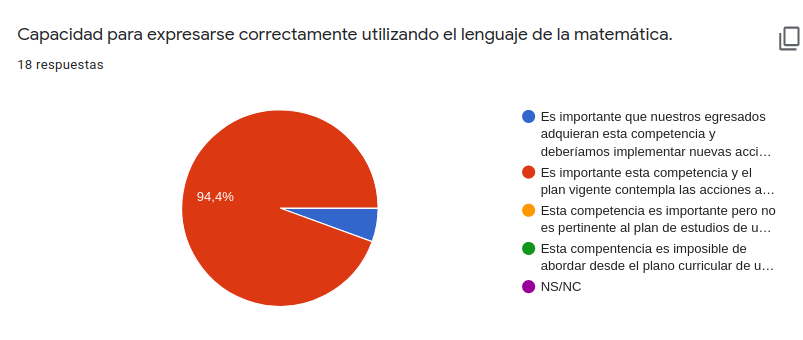
\includegraphics[scale=.9]{doc17.png}
 \end{center}
 
 
     \paragraph{Pregunta 18}
\begin{center}
 
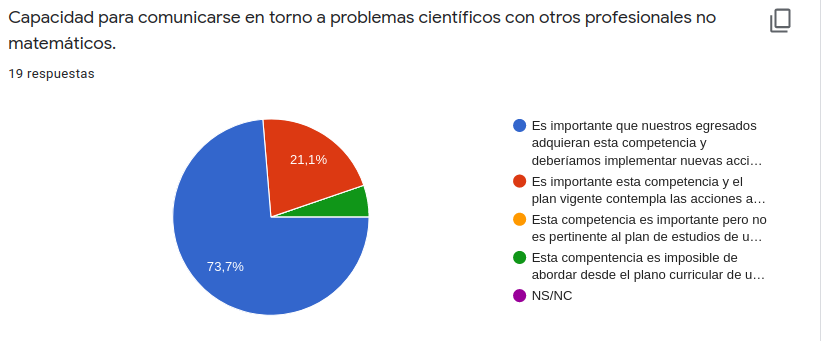
\includegraphics[scale=.9]{doc18.png}
 \end{center}
 
 
 En caso de haber elegido la primera opción en la pregunta anterior, que acciones puedes sugerir. Entendemos un rango amplio de acciones, como ser: nuevas materias-talleres-seminarios creados con el propósito específico, nuevas metodologías educativas, cambios en la orientación curricular, etc. 
 
 13 respuestas

 \begin{itemize} 
\item  Implementar acciones en cada asignatura

\item a) El cursado de asignaturas de otras carreras debería constituir una instancia favorecedora de esa comunicación b) La participación en instancias no formales como charlas (del estilo de "Café y Ciencia") sobre problemas de  otras disciplinas debería formar parte de la dinámica institucional usual.

\item Implementar nuevas metodologías en las asignaturas existes

\item Cursar alguna asignatura con ingenieros, computistas, biólogos, etc.

\item Deberíamos tener más trayectos compartidos con otras carreras, pero también es claro que es imposible abordar todos los espacios posibles

\item Es importante crear un espacio donde se trabaja multidisciplinariamente con otros profesionales (ingenieros, químicos, biólogos, etc) . Podría ser desde alguna asignatura  o algún taller 

\item Cursar alguna asignatura o taller con estudiantes de otras carreras afines a la matemática.

\item Nuestros alumnos deberían cursar asignaturas de otras carreras.

\item Podría haber algún taller o seminario inerdisciplinar. 
Seminarios o talleres en donde se realice intercambio con científicos de otras disciplinas.

\item Se puede pensar en espacios curriculares comunes con estudiantes de carreras como Ingeniería, Física, Computación u otras afines. 

\item Nuevamente considero fundamental esta competencia. También considero que hemos tenido intenciones de abordarla reconociendo espacios como el de Física, pero NO ALCANZA.  Mientras que no tensionemos una de las "patas de hierro" que sostiene nuestra organización docente universitaria, que es la atomización de los espacios curriculares , con intersección vacía entre el teórico y el práctico, no tenemos oportunidad de avanzar en el logro de estas capacidades o competencias co-disciplinares tan necesarias para entender además mejor que significa "hacer matemática". Se que no estoy poniendo una alternativa concreta de solución, sino propongo profundizar  un cambio de nuestras prácticas docentes.

\item En las asignaturas modelos matemáticos y las que se incluyan en relación a aplicaciones de la matemática, invitaría a profesionales de otras áreas tales como ingenieros, economistas, biólogos, químicos,  a que traigan problemas de su ciencia para que los estudiantes resuelvan.  
\end{itemize}
 
 
 
 
 
 
 
     \paragraph{Pregunta 19}
\begin{center}
 
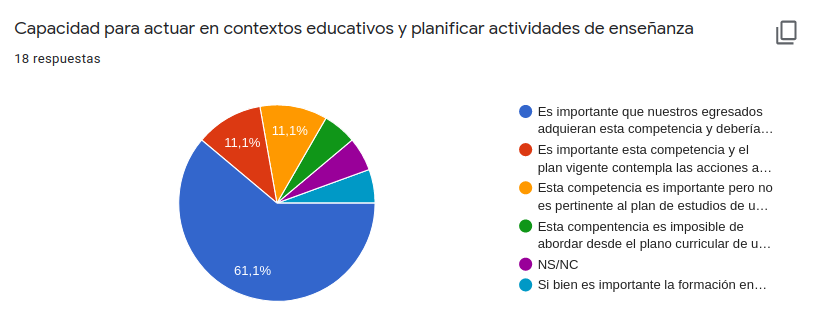
\includegraphics[scale=.9]{doc19.png}
 \end{center}
 
 
 
 
 
 En caso de haber elegido la primera opción en la pregunta anterior, que acciones puedes sugerir. Entendemos un rango amplio de acciones, como ser: nuevas materias-talleres-seminarios creados con el propósito específico, nuevas metodologías educativas, cambios en la orientación curricular, etc. 
 
 11 respuestas
 
 \begin{itemize}
\item  Implementar nuevas materias o talleres de formación pedagógica

\item  a) La formación didáctica y pedagógica debería transversalizar el currículo b) La promoción en la participación de nuestrxs estudiantes en las ayudantías de segunda es una política institucional a ser sostenida para tal efecto c) El cursado conjunto del profesorado y la licenciatura favorece el clima de valorización de la didáctica y la pedagogía como disciplinas científicas y como práctica social de gran valor 

\item  El licenciado en matemática se desempeña como docente (al menos eso sucede a la mayoría en nuestra universidad) pero sin embargo no han tenido ni un solo espacio para pensar en la enseñanza aprendizaje de la matemática, salvo aquellos que hayan realizado el profesorado con anterioridad. Es necesario nuevos espacios curriculares.

\item  Implementar Nuevas materias, seminarios o talleres

\item  Nuestra currículo debería contemplar algún espacio de reflexión sobre problemas de enseñanza. 

\item  Para contestar esta pregunta me parece que hay que tener bien en claro el perfil de egresado que se quiere.

\item  Considero que el perfil de egresado que se pretende formar no es para ir a dar clase al nivel medio, para esto hay una carrera especifica que es el profesorado. Pero hay una realidad que es que muchos licenciados terminan dando clase en el nivel superior. Yo no creo que sea necesario agregar materias especificas, creo que si se logra que los alumnos sean cada vez mas críticos, que puedan resolver diferentes tipos de problemas, que puedan usar herramientas computacionales, que puedan modelar y que además respeten la diversidad de la personas,  creo yo que van a ser profesionales con capacidad de planificar y enseñar.
Si estamos pensando a nuestro egresado con un perfil en el cual es probable que tenga que actuar en contextos educativos, creo que se debería incorporar una materia específica para esta capacidad.

\item  Es necesaria una formación específica para pensar y actuar en escenarios educativos, por lo que resultaría necesario un espacio creado con este objetivo.

\item  Que realicen practicas docentes en las materias de años anteriores a los que cursan dictadas por nuestro departamento. 

\item Practicas en varias materias de diretentes ramas para tener un amplio conocimiento de todos los temas.

\item Pienso a este ítems, como necesario para una de las salidas laborales del Licenciado en matemática. Y cuando pienso en un nivel dentro del sistema educativo donde puede actuar un licenciado, lo pienso al nivel universitario. Las problemáticas educativas de cada uno de los niveles exigen un conocimiento específico al que se debería acceder con responsabilidad institucional. Soy consciente que los propios Ministerios de Educación suelen violar estos principios, por ello estoy convencida que la política académica de las universidades deberían  tener mayor claridad al respecto y bregar por una formación específica para los docentes de cada nivel. Además en la actualidad hay un desarrollo de las didácticas específicas que sostienen y validan estas competencias específicas de los profesionales universitarios.
\item Incluiría algún espacio curricular pertinente
\end{itemize}




 
     \paragraph{Pregunta 20}
\begin{center}
 
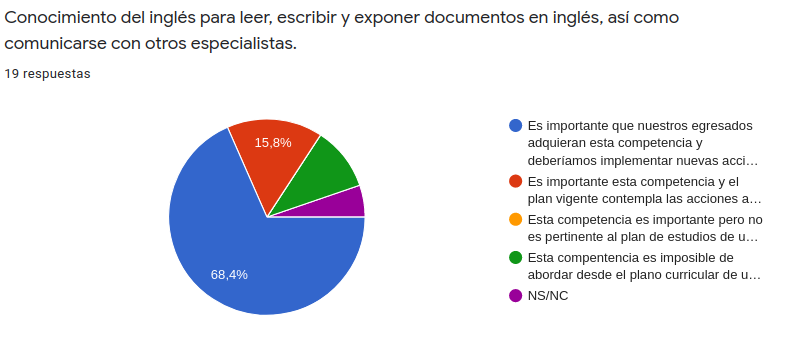
\includegraphics[scale=.9]{doc20.png}
 \end{center}
 
 En caso de haber elegido la primera opción en la pregunta anterior, que acciones puedes sugerir. Entendemos un rango amplio de acciones, como ser: nuevas materias-talleres-seminarios creados con el propósito específico, nuevas metodologías educativas, cambios en la orientación curricular, etc. 
 
 12 respuestas

 
 \begin{itemize}

 \item Implementar talleres específicos para el desarrollo de esta competencia. 
 
\item Implementar actividades en las asignaturas en donde necesiten leer y contar artículos en inglés 

\item a) Si bien existe el inglés como asignatura la utilización de textos en ese idioma en las asignaturas es una práctica a ser alentada b) Al mismo tiempo es importante alentar el estudio de otros idiomas, los cuales junto al inglés, pueden aprenderse de modo gratuito en UNRC c) En vistas de la perspectiva multicultural debe ser una política institucional enfatizar la importancia de estudios de lenguajes locales, de pueblos originarios

\item Deberían cursas 2 niveles de ingles, uno técnico y otro de comunicación oral.

\item Es necesario un curso de inglés general y otro técnico, según mi experiencia

\item Si bien los estudiantes cuentan con una asignatura, la misma esta muy alejada a las necesidades de  los estudiantes de matemática.  

\item Debería implementarse un taller o seminario donde se expongan trabajos en inglés, de manera de ejercitar la parte de exposición en este idioma.

\item Me parece importante que haya más cursos y talleres dedicados a otros idiomas.

\item El inglés que tiene la carrera es muy básico. No se si puede agregar otra materia que se aprendan contenidos de inglés (no se si vale la pena). Pero, tal vez no en primer año, pero si en años posteriores se le den trabajos a los alumnos en los que tengan que leer en inglés.

\item Sería necesario "revisar" el planteo actual del espacio específico existente en relación a esta competencia. Además se podría complementar la formación a partir de la posibilidad de plantear ciertos trabajo -que avancen en ese sentido- en algunos espacios de la carrera.

\item Se necesita más cursos de inglés obligatorios. Quizás una manera sea que los estudiantes puedan realizar algunos de los niveles de inglés que la universidad ofrece.  

\item No tengo claridad sobre la calidad de la enseñanza del inglés, pero en todo caso será cuestión de profundizar lo instituido.

\end{itemize}


     \paragraph{Pregunta 21}
\begin{center}
 
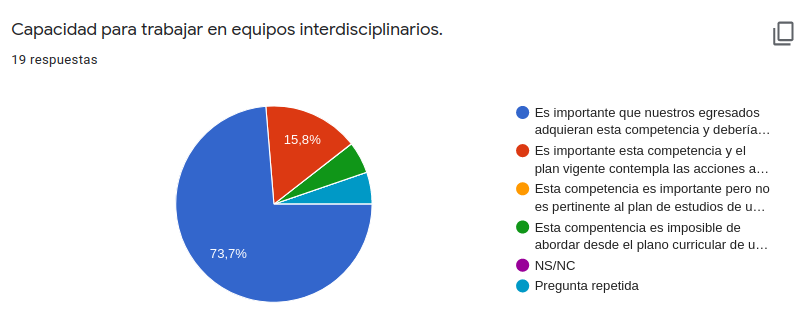
\includegraphics[scale=.9]{doc21.png}
 \end{center}
 En caso de haber elegido la primera opción en la pregunta anterior, que acciones puedes sugerir. Entendemos un rango amplio de acciones, como ser: nuevas materias-talleres-seminarios creados con el propósito específico, nuevas metodologías educativas, cambios en la orientación curricular, etc. 
 
 10 respuestas

 \begin{itemize}
\item  Implementar metodologías donde los alumnos interactúen con profesionales o alumnos de otras carreras
\item En espacios curriculares existentes, cambiar la metodología para lograr ésto
\item Es imposible cubrir todos los espacios, no me refiero a que no es importante. 
\item Nuestros alumnos deberían cursar materias de otras carreras
\item Creo que si formamos alumnos sólidos matemáticamente y con capacidad de modelar distintas situaciones problemáticas, van a estar capacitados para formar cualquier grupo interdisciplinar.
\item La posibilidad de estrategias que apunten, por ejemplo, a fortalecer el trabajo con problemas de "modelización" y "optimización", aportarían a la construcción de herramientas para una lógica de trabajo interdisciplinar.
Propongo nuevamente participacion en los trabajos de investigacion.
\item Participar en grupos interdisciplinarios en la solución de problemas regionales, nacionales, entre otros, es una habilidad importante que debe ser adquirida por un Licenciado en Matemáticas. Quizás se pueda implementar una experiencia profesional una vez aprobado un cierto porcentaje de la carrera. 
\item Esta es otra de las capacidades que se tuvieron presente para hacer el plan vigente. Por lo que reflexionar sobre lo alcanzado y sobre ello pensar en lo que falta, pienso que es un camino más que fructífero a recorrer. Además nuestro Departamento se ha consolidado estos últimos años, en el camino de la investigación interdisciplinaria, lo que ayuda a imaginarnos un escenario muy potente para pensar nuevas actividades con los estudiantes  que complementarían a las ya instituidas en las asignaturas construidas  para tal fin. 
\item Mi respuesta va en consonancia con lo respondido en "Capacidad para comunicarse en torno a problemas científicos con otros profesionales no matemáticos"

\end{itemize}



     \paragraph{Pregunta 22}
\begin{center}
 
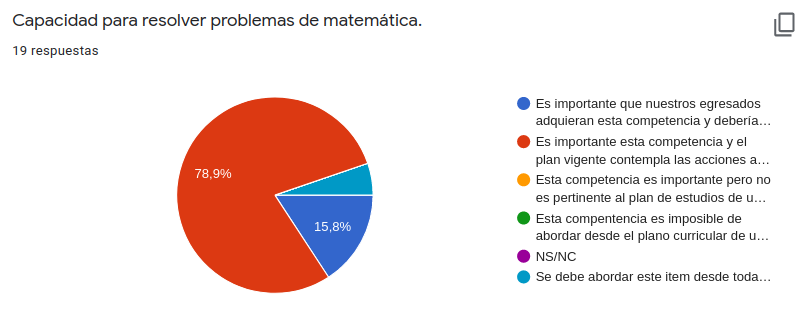
\includegraphics[scale=.9]{doc22.png}
 \end{center}
 
 En caso de haber elegido la primera opción en la pregunta anterior, que acciones puedes sugerir. Entendemos un rango amplio de acciones, como ser: nuevas materias-talleres-seminarios creados con el propósito específico, nuevas metodologías educativas, cambios en la orientación curricular, etc. 
 
 3 respuestas

 \begin{itemize}
  \item Debería implementarse en cada espacio curricular
  \item Implementar nuevas metodologías en espacios curriculares existentes 
  \item Hay que ejercitar al alumno en esta dirección proponiéndole   problemas desafiantes y adecuadas a su etapa formativa. 
 \end{itemize}

      \paragraph{Pregunta 23}
\begin{center}
 
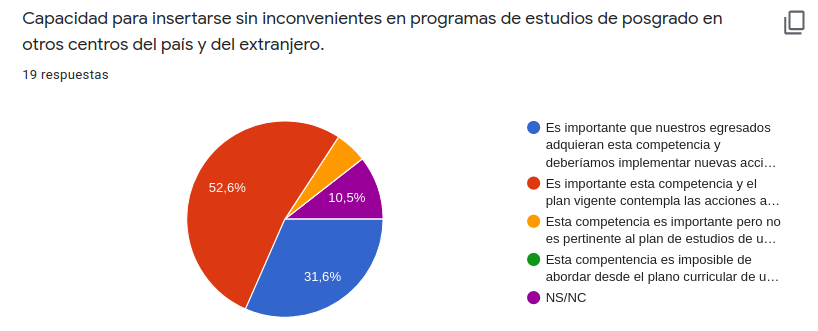
\includegraphics[scale=.9]{doc23.png}
 \end{center}

   En caso de haber elegido la primera opción en la pregunta anterior, que acciones puedes sugerir. Entendemos un rango amplio de acciones, como ser: nuevas materias-talleres-seminarios creados con el propósito específico, nuevas metodologías educativas, cambios en la orientación curricular, etc. 
   
   6 respuestas

   \begin{itemize}
    \item   En el diseño del plan de estudio tener en cuenta los conocimientos y planes de estudios de grado de otras universidades  y los requerimientos de las carreras de posgrado, por lo menos en la región
    \item La formación matemática la considero sólida, el conocimiento de idioma extranjero es relativo a la persona y lo demás dependerá de los requerimientos de cada institución y carrera de posgrado que se decida hacer. No podría responder con seguridad si se logra o no la capacidad que se consulta.
    \item Tener en cuenta los contenidos solicitados en otros centros de estudio, para incorporarlo en los espacios curriculares existentes y asegurarse que los egresados posean los mismos
    \item Podría generarse un ciclo de charlas con ex estudiantes para que cuenten su experiencia en la búsqueda de becas, experiencias etc. 
    \item Hay que estudiar los programas de estudio de otras instituciones.  
    \item  Debemos formar matemáticos con bases sólidas en las principales áreas de las matemáticas que permitan a nuestros egresados sin un mayor esfuerzo incorporarse a otros programas de estudios del país o del extranjero. 

   \end{itemize}

 









 \end{subappendices}
 
 
\chapter{Propuestas innovación curricular}

\section{Análisis Matemático}

\subsection{Introducción y fundamentación}

 Un problema que se presenta en nuestros planes de estudio, entendidos estos en un sentido amplio, es el supuesto que la mejor forma de trasmitir un saber es trasmitir su formalización y que por tanto, cuanto más  correcto en el sentido formal se exponga un determinado tema, más claro será éste para los estudiantes. Según esta óptica no es relevante indagar sobre los medios con los que se llegó al conocimiento sino su justificación.    No es nuestra intención negar la importancia de la instancia formalizadora, después de todo ella es uno de los aspectos que nos distinguen del resto de las ciencias y quizás el día de mañana esta característica posibilite que las máquinas desarrollen matemática de manera autónoma.  Lo que se pretende poner en discusión es  la manera de llegar a un conocimiento o de aprender un concepto. Pensamos que esto contempla diversas etapas, de las cuales formalizar es una, pero creemos que intervienen otras sobre la que es necesario trabajar de manera consciente con los estudiantes.
 
La historia de la matemática ofrece abundante material para la discusión del punto planteado. Por ejemplo, el concepto de límite fue formalizado por Cauchy durante las primeras décadas del siglo 19. Sin embargo, desde la remota antig\"uedad,  a los matemáticos les aparecieron problemas que llevaban a la idea de límite. El problema de asignar áreas a figuras planas es uno de ellos, o el de calcular números o funciones trascendentes, ejemplo $\pi$, funciones trigonométricas, raíces cuadradas, etc. Llegar a formalizar la idea de límite, implicó primero entender que los procedimientos de cálculo por aproximaciones definían  un objeto. Esto es que del infinito potencial se puede pasar al infinito actual, en otras palabras  concebir el procedimiento de aproximación acabado. Se planteó luego la necesidad de conceptualizar esta idea de límite, en esta conceptualización se fueron dando diversas propuestas de explicarlo o definirlo hasta llegar a la definición actual. 

Recientemente ha surgido una variada bibliografía exponiendo propuestas de enseñanza de la matemática guíada por considereaciones históricas. Cabe aclarar que no nos referimos a estudios de la historia de la matemática, o a matizar la enseñanza con comentarios históricos más o menos anecdóticos,  sino a libros que pueden ser utilizados a la hora de diagramar una clase.  Citamos algunos de estos materiales  en el área del análisis matemático: \cite{hairer_history,shell_from,bressoud_anal,bressoud_lebes, toeplitz,Bressoud_compend}.

A la vez pensamos que el saber matemático no es sólo la acumulación de conocimientos, sino más bien la apropiación de ciertas competencias que caracterizan al matemático. La mayor parte de ellas se ponen en juego al momento de resolver un problema. George Polya en \cite{polya_how,polya_plauI,polya_plauII} ha caracterizado algunas estrategias y métodos heurísticos que se ponen en juego cuando se resuelve un problema, la inducción (en el sentido empírico, no la inducción matemática), la analogía, plantear problemas más simples, etc. 

También detectamos, que unas de las dificultades que se presenta en el primer año de la carrera es la de redefinir conceptos estudiados en el secundario. Por tal motivo proponemos, por ejemplo, el libro \cite{bocco}. En él se abordan las funciones a partir de problemas que modelizan situaciones reales. La matemática, que muchos describen como "el lenguaje del universo", nos otorga
la posibilidad de describir, calcular y predecir el comportamiento del mundo que
nos rodea. Consideramos que la bibliografía 

Por todo ello, pensamos que es necesario fortalecer todas nuestras asignaturas en cuanto a la resolución de problemas. Cuando decimos problemas, nos referimos a un problema matemático que ponga en juego las estrategias de Polya. Así ejercicios del tipo: hallar los $x\in\mathbb{R}$ tales que $0<|3x-1|<6$ no son problemas en el sentido anterior, dado que el ejercicio sólo pone en juego la capacidad del alumno de ejecutar una secuencia de pasos que luego de resolver algunos ejercicios similares se convierte en mecánica. Puede que los alumnos tengan dificultades en resolver estos ejercicios, esto en todo caso dice que la mecánica de solución es compleja para ellos, pero no por ello dejó de ser mecánica. Además el resultado que se aspira hallar se encuentra descontextualizado, en el sentido que es difícil de explicar por qué queríamos resolver dicho ejercicio. Todos fuimos expuestos a este tipo de cálculos, la explicación quizás se encuentre en que los usamos de preparatorios de la definición de límite donde se emplean desigualdades con módulo. Es oportuno aclarar que no estamos sosteniendo que deban erradicarse este tipo de actividades. Si queremos remarcar cómo la enseñanza tradicional (por llamarla de algún  modo) fue diagramada para satisfacer las necesidades de la formalización, un objetivo central de los cálculos, es llegar a la definición formal de límite y mucho del planteo pedagógico tiende a satisfacer aquella necesidad.  
 
Distinto es el caso de por ejemplo el siguiente problema muy conocido.  Hallar una expresión cerrada para la suma de los primeros $n$ naturales, $1+2+\cdots+n$. El problema es interesante en si mismo, se lo podemos explicar con facilidad a prácticamente cualquier persona y además es desafiante su solución. Quizás el alumno deba planear una estrategia para, en primer lugar, hallar la fórmula. Quizás usará la inducción de Polya. Luego intentará justificarla. Allí influirá si conoce o no el principio de inducción. En este ejemplo se observa cuánta distancia hay entre justificación y descubrimiento. Si se dispone del resultado su justificación mediante el principio de inducción es mecánica. Pero conocer la respuesta de antemano es un problema en si mismo más difícil que justificar la veracidad de la respuesta. Es común que veamos este tipo de ejercicios con la respuesta ya dada, es decir enunciándolo de la siguiente forma: demostrar que $1+2+\cdots+n=n(n+1)/2$. De esta manera evitamos que los alumnos desarrollen estrategias de descubrimiento y a nosotros como docentes se nos simplifica el diagramado de las clases, pues no nos preocupamos de cómo  desarrollar esa competencia en los alumnos.  


Ya que venimos hablando de sumatorias de una cantidad finita y arbitraria de términos, queremos sostener que un aspecto muy importante  de trabajar con ellas es que sirve de  preparación para abordar series infinitas. 

La capacidad de hallar expresiones cerradas para sumas finitas o infinitas no es una competencia que aparezca como muy importante en nuestros planes de estudio y en la bibliografía. Esto es misterioso, porque luego de introducir series infinitas, la bibliografía  pasa directamente a discutir métodos indirectos para justificar su convergencia. ¿Por qué se hace esto? Si la manera más directa, en principio,  de justificar la convergencia de una serie es expresar las sumas parciales de manera exacta y calcular su límite. Esto es lo que haría cualquier persona que entendió la definición de convergencia de serie.   Evidentemente la respuesta se halla en la dificultad que hay en encontrar expresiones cerradas para sumas.  Pero esa dificultad no la ha vivenciado un alumno del primer año de nuestra carrera y posiblemente a lo largo de la carrera nunca se enfrente de manera sistemática con este tipo de cuestiones.






\subsection{Contenidos y metodología de precálculo}

En esta sección describimos los contenidos a desarrollar en -Precálculo, espacio curricular situado en el primer cuatrimestre del primer año, y algunos problemas que nos parecen interesantes desarrollar para arribar a dichos contenidos. 
No nos proponemos reproducir la historia de la matemática, pero sí usar como principio director que debemos plantear al alumno problemas que tengan sentido para él, esto es, que sea capaz de entenderlos y de juzgar su importancia, que perciba que hay una lógica en el desarrollo de la matemática y en tratar de motivar los temas introducidos mostrando que vienen a dar respuesta a estos problemas o interrogantes de los que el estudiante se puede apropiar. Nos sirvió de  guía el texto \cite{hairer_history}. 

\textbf{No es nuestra intención por el momento elaborar notas de clases, sino más bien presentar una posible dirección para arribar a los contenidos. El plan final de la unidad temática Precálculo podría o no desarrollar estos problemas, pero sí debería conservar el planteo filosófico.}  

Nos proponemos además pantearles problemas que impliquen un desafío, atendiendo a la altura de la carrera en que 
se presupone estará la unidad y que ese desafío se restrinja a usar de manera un  poco ingeniosa  manipulaciones algebraicas.

Otra consideración importante es que en \textbf{Precálculo se deben desarrollar problemas que muestren la necesidad de introducir el concepto de límite.} La consigna es mostrar varios ejemplos donde la única manera de expresar la solución que tenemos es por medio de un proceso infinito.






\subsection{Teorema del Binomio y la función $e^x$}

\textbf{El objetivo de esta sección es definir la función exponencial $e^x$. Para lograrlo elegimos hacerlo a través del Teorema del Binomio y definiendo el número de Euler denotado por $e$. Como consecuencia de introducir el binomio de Newton obtendremos además la construcción de las funciones $a^x$, donde $a>0$ y $x$ racional. Más adelante, después de definir las funciones logarítmicas podremos definir las funciones $a^x$, para cualquier $x$ real.}

Sea $a$ un número dado, $a>0$, podemos escribir la siguiente "sucesión" de números: 

\begin{equation}\label{2.1}
a.a=a^2, \quad a.a.a=a^3, \quad a.a.a.a=a^4, ...
\end{equation} 

Esta notación surge del trabajo de Bombelli en $1572$, Stevin en $1585$, Descartes y Newton. Ahora si multiplicamos $a^2$ y $a^3$, obtenemos $$a^2.a^3=(a.a).(a.a.a)= a.a.a.a.a=a^5,$$
y con un procedimiento similar, podemos demostrar la regla

\begin{equation}\label{2.2}
a^n.a^m=a^{n+m}.
\end{equation} 

En (\ref{2.1}) vemos que cada término es igual a su anterior multiplicado por $a$. De la misma manera podemos continuar esta secuencia hacia la izquierda dividiendo el término anterior por $a$. Esto lleva a:
$$...\quad a^{-2}=\frac{1}{a.a},\quad a^{-1}=\frac{1}{a},\quad a^0=1,\quad a^1=a,\quad a^2=a.a,\quad...$$
donde usamos la notación 

\begin{equation}\label{2.3}
a^{-m}=\frac{1}{a^m}.
\end{equation} 

De esta manera, la fórmula (\ref{2.2}) sigue valiendo para exponentes negativos. Por otro lado, multiplicando $1$ repetidamente por $\sqrt{a}$ (siendo $a$ un número positivo) obtenemos una progresión geométrica 
$$1, \quad \sqrt{a}, \quad \sqrt{a}.\sqrt{a}=a, \quad \sqrt{a}.\sqrt{a}.\sqrt{a}=\sqrt{a^3}, \quad \sqrt{a}.\sqrt{a}.\sqrt{a}.\sqrt{a}=\sqrt{a^4}=a^2, \quad ...$$

Lo cual sugiere la notación

\begin{equation}\label{2.4}
a^{\frac{m}{n}}=\sqrt[n]{a^m}.
\end{equation} 

Ahora la fórmula (\ref{2.2}) sigue valiendo también para exponentes racionales.

\textbf{Observemos que en este procedimiento estamos usando propiedades de la raiz cuadrada y el hecho de que sabemos calcular $\sqrt[n]{a}$, donde $a>0$, porque se ha definido previamente en el nivel medio (lo cual puede repasarse en este instante ya que hemos definido la operación $a^n$). No estamos introduciendo, por ejemplo, la función $\sqrt{x}$, aunque puede hacerse como consecuencia.}

El paso siguiente sería pensar repetir este procedimiento para exponentes irracionales (por ejemplo $a^{\sqrt{7}}$), lo cual, según Euler, $"$esto es un poco más difícil de entender". Luego, no definiremos $a^x$ para $x$ irracional de esta manera, sino que saldrá como consecuencia de haber estudiado función logaritmo, en la próxima sección.

Ahora nuestro objetivo es demostrar un teorema (Pascal 1654) para poder definir la función exponencial de base $e$ en todos los reales.

Supongamos que deseamos expandir $(a+b)^n$. Realizando una multiplicación sucesiva, obtenemos:

\begin{equation}
\begin{tabular}{|c|} \hline 
$(a+b)^0=1$ \\
\hline 
$(a+b)^1=a+b$ \\ 
\hline 
$(a+b)^2=a^2+2ab+b^2$ \\ 
\hline 
$(a+b)^3=a^3+3a^2b+3ab^2+b^3$ \\ 
\hline 
$(a+b)^4=a^4+4a^3b+6a^2b^2+4ab^3+b^4$ \\ 
\hline 
... \\
\hline 
\end{tabular} 
\end{equation}
 
Apareciendo un interesante triángulo de coeficientes binomiales (Pascal 1654) como se muestra en la figura siguiente, en el cual cada número es la suma de $"$sus dos superiores". 

 \begin{figure}[h!]
    \centering				                     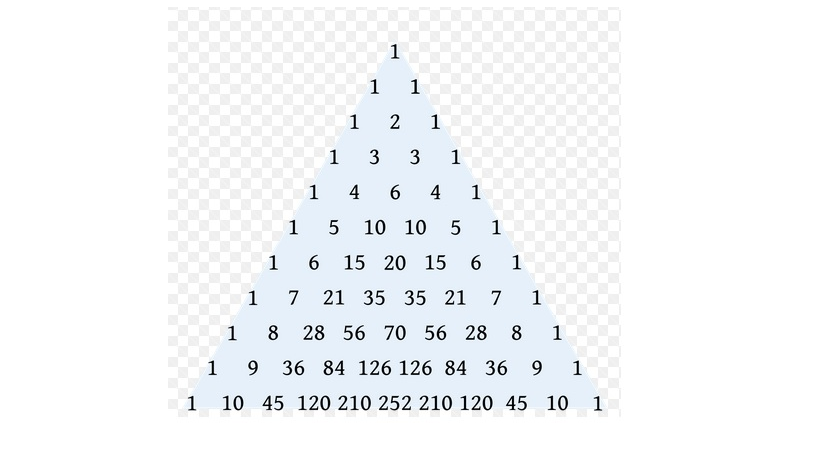
\includegraphics[width=0.80\linewidth]{triang2.png}
 \end{figure}

Además, mirando cada diagonal, introduciendo la noción de factorial y definición de número combinatorio, se puede demostrar el siguiente teorema.

\textbf{Teorema:}
Para cada $n=0,1,2...$ tenemos 
\begin{equation}\label{teorema2.1}
 (a+b)^n=\sum_{k=1}^n\binom{n}{k} a^kb^{n-k},\quad n\in\mathbb{N}.
\end{equation}

Realicemos algunas observaciones sobre la fórmula del binomio de Newton:
\begin{itemize}
 \item Es la generalización natural de la fórmula que es  bien conocida por cualquier alumno de enseñanza media $(a+b)^2=a^2+2ab+b^2$.
 \item Su justificación entraña técnicas de conteo, relacionando el álgebra con la combinatoria.
 \item Simples argumentos heurísticos, ver  \cite{hairer_history}, muestran que cuando queremos poner exponentes $n$ que no son enteros positivos deberíamos considerar expresiones con límites. Por ejemplo, como actividad curricular concreta, podemos proponer hallar una fórmula para $(1+x)^{-1}$. Como estrategia heurística de descubrimiento proponer continuar la división polinomial de $1$ por $1-x$. Si bien se conviene en deterner el proceso de división cuando uno arriba a un polinomio de grado menor al divisor, no es incorrecto continuarla, de la misma manera que cuando dividimos enteros podemos continuar la división después de llegar a un resto menor que el divisor agregando una coma al cociente. Arribaremos a la interesante conclusión 
  \[
  \begin{array}{lllll} 
  1  &    &       &             & \multicolumn{1}{|l}{1-x}\\ \cline{5-5}
  1  & -x &       &             & 1 +x+x^2+\cdots  \\ \cline{1-2} 
     &  \phantom{-}x &       &             &        \\  
     & \phantom{-}x  & -x^2  &             &        \\ \cline{2-3}
     &               & \phantom{-}x^2      &        \\ 
     &               & \phantom{-}x^2      & -x^3   \\ \cline{3-4}
     &               &                     & \phantom{-} x^3 \\
     &                &                    &  \phantom{-}\vdots         \\
    \end{array}
\]
 
 Claramente el proceso no termina nunca, los restos sucesivo son $1,x,x^2,x³,\ldots$ y el cociente $1+x+x^2+\cdots$.  Aquí se puede pedir que los alumnos experimenten numéricamente sobre como los sucesivos cocientes parciales van aproximando el cociente. También preguntarles si los restos $1,x,x^2,\ldots$ serán números grandes o pequeños. 
 
 Queremos hacer una digresión aquí. Si bien los experimentos empíricos que proponemos se pueden desarrollar con una simple calculadora, 
 se hace imperioso que  los alumnos dispongan lo antes posible de  recursos en  programación que permitirían  llevar adelante estas experimentaciones en computadoras o aún en smartphones. 
 
Volviendo al punto principal, en síntesis la idea es que los alumnos vayan intuyendo la fórmula
 \[\frac{1}{1-x}=\sum_{n=0}^{\infty}x^n,\]
 por medio del razonamiento heurístico propuesto u otro y por medio de la evidencia empírica. La fórmula obviamente será justificada con todo el rigor al finalizar el cuatrimestre.  
\end{itemize}

\textbf{A continuación, siguiendo con la misma idea, comenzaremos a trabajar de manera heurística con la noción de límite. Observaremos que hay que ser cuidadoso en el razonamiento empleado y que todo será devidamente justificado en la última sección del precálculo (y mucho más estudiado el próximo cuatrimestre).}

\title{Número de Euler}
 Aplicando la fórmula del binomio dada en (\ref{teorema2.1}) obtenemos:
\[(1+\frac{1}{N})^N=1+\frac{N}{N}+\frac{N(N-1)}{1*2}*\frac{1}{N^2}+\frac{N(N-1)(N-2)}{1*2*3}*\frac{1}{N^3}+\dots\] \[=1+1+\frac{1(1-\frac{1}{N})}{1*2}+\frac{1(1-\frac{1}{N})(1-\frac{2}{N})}{1*2*3}+\dots, \]

y Euler observa que si $N$ es suficientemente grande, entonces $\frac{N-1}{N}$ es $"$igual$"$ a $1$, ocurriendo lo mismo con los factores similares como $\frac{N-2}{N}$, $\frac{N-3}{N}$, etc. Esto de pensar en $N$ grande es hacer tender $N$ al infinito, y así, $(1+\frac{1}{N})^N$ tiende al llamado número de Euler:

\begin{equation}\label{2.17}
(1+\frac{1}{N})^N \stackrel{N \rightarrow \infty}{\longrightarrow} 1+1+\frac{1}{1*2}+\frac{1}{1*2*3}+\frac{1}{1*2*3*4}+\dots :=e
\end{equation}

\textbf{Este argumento es peligroso en el sentido que}
\[1=\frac{1}{2}+\frac{1}{2}=\frac{1}{3}+\frac{1}{3}+\frac{1}{3}=\frac{1}{N}+\frac{1}{N}+\dots+\frac{1}{N}=0+0+\dots+0=0!!\]

\textbf{Observación: hay que tener y diferenciar sumas finitas e infinitas. Por tal motivo, vemos necesario cerrar el Precálculo con la justificación de estos procedimientos, introduciendo los conceptos de sucesión, serie numérica y convergencia.}

Continuando con el mismo razonamiento para el número de Euler, podemos definir la potencia de $e$, es decir la función $e^x$ como sigue:

\begin{equation}
\label{2.18}
(1+\frac{x}{N})^N \rightarrow 1+x+\frac{x^2}{1*2}+\frac{x^3}{1*2*3}+\frac{x^4}{1*2*3*4}+...
\end{equation}

Por otro lado, llamando $M=\frac{N}{x}$ y suponiendo que la función que queremos definir tiene cierta propiedad obtenemos:

\begin{equation}
\label{2.19}
(1+\frac{x}{N})^N=(1+\frac{1}{M})^{Mx}=((1+\frac{1}{M})^M)^x \rightarrow e^x.
\end{equation}

Con lo cual, de (\ref{2.18}) y (\ref{2.19}) obtenemos el seguiente Teorema:

\textbf{Teorema (Euler 1748):} Para $N$ tendiendo al infinito  
$$(1+\frac{x}{N})^N \rightarrow e^x=1+x+\frac{x^2}{1*2}+\frac{x^3}{1*2*3}+\frac{x^4}{1*2*3*4}+...$$

\textbf{Observación: la unicidad del límite será justificada más adelante, quizás de forma general cuando se trabaje con límite de funciones en el segundo cuatrimestre o se puede realizar la prueba para sucesiones en la última sección.}

La convergencia de estas expresiones a $e^x$ se ilustran en la figura siguiente. 

\begin{figure}[h!]
\centering
    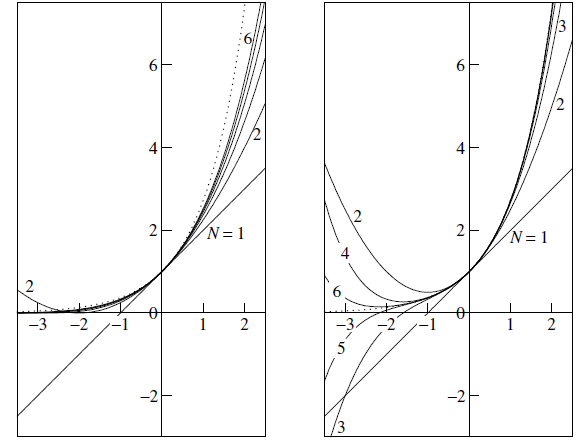
\includegraphics[width=0.4\linewidth]{exp1.png}
  %\caption{Mi Figura}
  \label{fig:exp}
\end{figure}


\newpage
\subsection{Función Logaritmo y Exponenciales de base $a$} 

M.Stifel(1544) resalta el siguiente hecho:
Dada la tabla a continuación,
\begin{figure}[h!]
\centering
    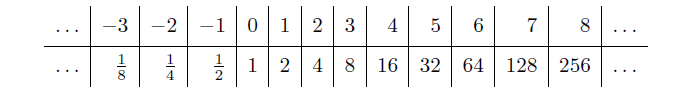
\includegraphics[width=0.8\linewidth]{log1.png}
  %\caption{Mi Figura}
  \label{fig:log}
\end{figure}

se pueden transformar productos en sumas, por ejemplo: si queremos multiplicar $8*32$ hacemos $3+5$ (los correspondientes "logaritmos" de 8 y 32 respectivamente) y el resultado es $8$. Nos fijamos en la tabla y resulta que $8*32=256$.

Así, las tablas logarítmicas fueron utilizadas para transformar productos en sumas.

\textbf{Definición}: Una función $l(x)$ definida para valores positivos de x, es llamada función logaritmo si para todo $x,y>0$:
\begin{equation}
l(x*y)=l(x)+l(y)
\label{eq1}
\end{equation}

Si tomamos $y=\frac{z}{x}$, con $x=y=1$ en (\ref{eq1}) obtenemos:

\[\    l(\frac{z}{x})=l(z)-l(x)\]
\[  l(1)=0\]
    

Aplicando (\ref{eq1}) dos veces a $x*y*z=(x*y)*z$ obtenemos:
\begin{equation}
    l(x*y*z)=l(x)+l(y)+l(z)
    \label{eq4}
\end{equation}
y similarmente para productos de 4 factores o más.
Luego aplicando \ref{eq4} a
\[\sqrt[3]{x}\sqrt[3]{x}\sqrt[3]{x}=x\]
tenemos $l(\sqrt[3]{x})=\frac{1}{3}l(x)$ o en general:
\begin{equation}
    l(x^{\frac{m}{n}})=\frac{m}{n}l(x) \;donde \;x^{\frac{m}{n}}=\sqrt[n]{x^m}
    \label{eq5}
\end{equation}

\textbf{Bases}: Sea una función logarítmica fija $l(x)$ y suponemos que existe un número $a$ para el cual $l(a)=1$ entonces por (\ref{eq5}) tenemos:
\[  l(a^{\frac{m}{n}})=\frac{m}{n}\]
es decir, la función logaritmo es la inversa de la función exponencial $a^x$ (definida para $x$ racional) y llamaremos $a$ a la base del logaritmo, escribiendo:
\begin{equation}
    y=\log_{a}(x)\Leftrightarrow x=a^y
    \label{eq6}
\end{equation}

Los logaritmos de base 10 son los más adecuados para cálculos numéricos, ya que un desplazamiento del punto decimal simplemente agrega un número entero al logaritmo. La mejor base para un trabajo teórico, es el número de Euler, '$e$' \;(dicho logaritmo recibe el nombre de "natural","Naperiano","hiperbólico") y se denota por $\ln(x)$.

\textbf{Regla de oro de Euler}: Si el logaritmo para cierta base es conocido, entonces el logaritmo para todas las bases es obtenido por una simple división. Para ver esto, tomemos el logaritmo de base $b$ de $x=a^y$ y usemos (\ref{eq5}) y (\ref{eq6}), entonces
\[
    \log_{b}(x)=\log_{b}(a^y)=y\log_{b}(a)\]
luego
    
\[ \log_{b}(x)=y\log_{b}(a)=\log_{a}(x)\log_{b}(a) 
    \]
Con lo cual obtenemos:
\begin{equation}
    y=\log_{a}(x)=\frac{\log_{b}(x)}{\log_{b}(a)} 
\end{equation} 

A continuación se puede demostrar que $\ln(x)=\log_{e}(x)$ (Teorema 3.3 de Analysis by Its History pág.38) y finalmente, para cerrar con las funciones logarítmicas y exponenciales, definir las potencias para un exponente arbitrario (pudiendo ser irracional) como sigue.

Supongamos que $a=e^{\ln(a)}$, entonces
\[a^b=(e^{\ln(a)})^{b}=e^{b\ln(a)}\]
y así hemos definido la función exponencial para cualquier numero real.

Gráficos de funciones de este tipo pueden verse en la figura que sigue:

\begin{figure}[h!]
\centering
    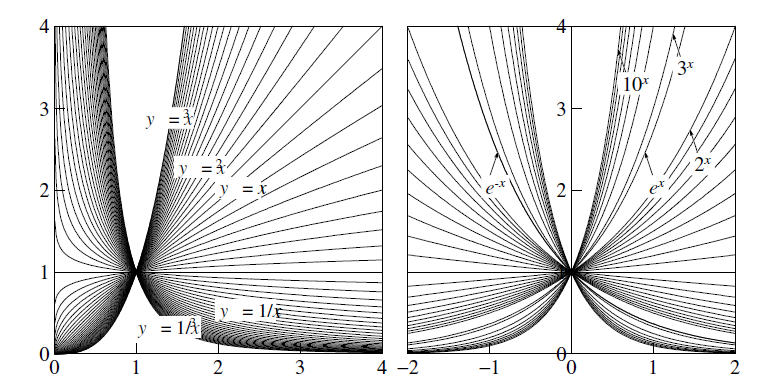
\includegraphics[width=0.7\linewidth]{exp2.png}
  %\caption{Mi Figura}
  \label{fig:exp}
\end{figure}

\newpage
\subsection{Funciones Trigonométricas} 

Uno de los primeros problemas de la geometría fue medir ángulos. Los Babilonios dividieron el círculo en 360º, probablemente por ser la cantidad aproximada de días del año, el tiempo que tarda la tierra en dar una vuelta al sol. Tiempo después, Ptolomeo redifinió la medida incluyendo dígitos en el sistema numérico en base 60, llamados minutos y segundos.

Pero los grados no son la única opción para medir ángulos, existe una medida natural, basada en la longitud de la circunferencia de radio uno, el radián. Aquí, la longitud del arco de la mitad del círculo es, con la precisión calculada por Lagny en 1719 y reproducida por Euler: 3,1415926535...

Para esta expresion algo difícil de manejar, W. Johns (1706) introdujo la abreviatura $\pi$. Luego el ángulo de 54º dibujado en la figura \ref{fig:ejemplo} mide $\frac{54\pi}{180}$ radianes.

\begin{figure}[h!]
  \centering
    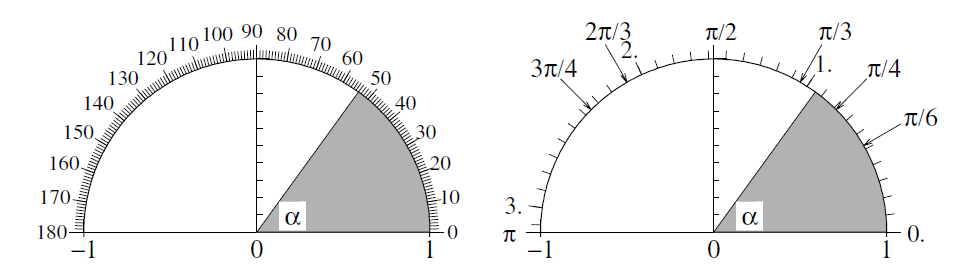
\includegraphics[width=95mm]{grados.png}
  %\caption{Mi Figura}
  \label{fig:ejemplo}
\end{figure}

\subsection{Definición}

Si se considera un triángulo rectángulo en un círculo de radio uno, como se muestra en la próxima figura, se tine que la longitud del lado opuesto al ángulo $\alpha$ se denota por $sen(\alpha)$ y la del lado adyacente por $cos(\alpha)$. Sus cocientes son las longitudes de las tangentes verticales y horizontales al circulo. 
%\[tan(\alpha)=\frac{sin(\alpha)}{cos(\alpha)} \ \ \ \ \
%cot(\alpha)=\frac{cos(\alpha)}{sin(\alpha)}\]


\[tan(\alpha)=\frac{sen(\alpha)}{cos(\alpha)} \ \ \ \ \ cot(\alpha)=\frac{cos(\alpha)}{sen(\alpha)}\]

\begin{figure}[h!]
\centering
    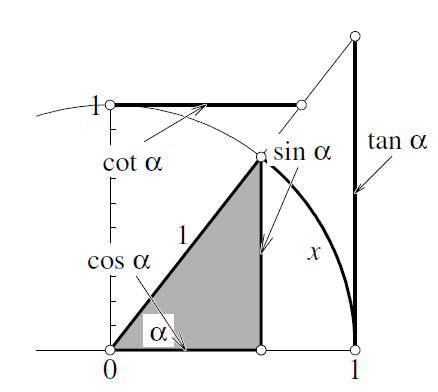
\includegraphics[width=0.35\linewidth]{trigonometria.png}
  %\caption{Mi Figura}
  \label{fig:ejemplo1}
\end{figure}






Estas definiciones se extienden inmediatamente a un triángulo rectángulo arbitrario con hipotenusa $c$ lados $a$ y $b$ (con $a$ opuesto al ángulo $\alpha$) como sigue 
\[ a=c*sen(\alpha)\ \ \ b=c*cos(\alpha) \ \ \
a=b*tan(\alpha) \]


Mientras que en geometria los ángulos se denotan con letras griegas, cuando consideramos radianes, las funciones son de variable real y preferimos nombrar el argumento con letras latinas minúsculas. Observando la figura se puede deducir que
\[sen(0)=0 \quad cos(0)=1 \quad sen(\pi/2)=1 \quad cos(\pi/2)=0 \quad sen(\pi)=0 \quad cos(\pi)=1\] Además
\[ sen(-x) = -sen(x)\ \ \ cos(x) = cos(-x)  \]
\[ sen(x+\pi) = -sen(x)\ \ \ cos(x+\pi) = -cos(x)  \]
\[sen(x + \frac{\pi}{2}) = cos x\ \ \ cos(x + \frac{\pi}{2}) = -sen x  \]
\[ sen(x)^2+cos(x)^2 =1  \]

Observemos que las funciones $sen(x)$ y $cos(x)$ son periódicas de periodo $2\pi$, mientras que la función $tan(x)$ es periódica de periodo $\pi$.

Los gráficos de estas funciones reproducen el dibujo de la curva sinusoidal de D$\ddot{u}$rer (1525) que se muestra a continuación. Si bien se pueden introducir dichos gráficos en este momento, la idea es expandirlas en serie y obtener sus gráficas a partir de estas series.

\begin{figure}[h!]
\centering
    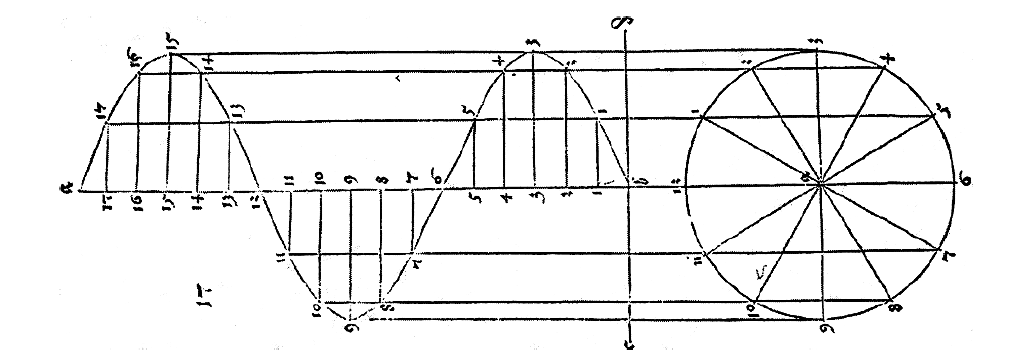
\includegraphics[width=1\linewidth]{trig2.png}
  %\caption{Mi Figura}
  \label{fig:ejemplo1}
\end{figure}

A continuación, podemos demostrar el siguiente Teorema, utizando solo las definiciones dadas anteriormente.

\textbf{Teorema}. \begin{equation}\label{4.3}
sen(x+y)=sen(x)cos(y)+cos(x)sen(y)
\end{equation} 
\begin{equation}\label{4.4}
cos(x+y)=cos(x)cos(y)-sen(x)sen(y)
\end{equation} 

Para la demostraciòn de este Teorema basta ver la imagen siguiente.

 \begin{figure}[h!]
    \centering				                     	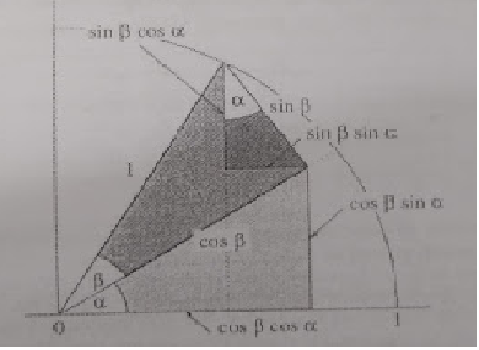
\includegraphics[width=0.60\linewidth]{teortrig.png}
\end{figure}

Aplicando este Teorema, podemos obtener las siguientes fómulas, conocidas como las Fórmulas de Moivre.

\begin{equation}\begin{split} \label{4.12 y 4.13}
& sen((n+1)x)=sen(x)cos(nx)+cos(x)sen(nx) \\
& cos((n+1)x)=cos(x)cos(nx)-sen(x)sen(nx)
\end{split}
\end{equation} 

Cuando reemplamos $n$ de las fórmulas anteriores por $1,2,3,4,etc$ aparece nuevamente el triángulo de Pascal a la derecha de la igualdad, y siguiendo como en el Teorema \ref{2.1} obtenemos las fórmulas generales de Moivre:

\begin{equation}\begin{split} \label{4.14}
& cos(nx)=cos^n(x)-\frac{n(n-1)}{1*2}sen^2x cos^{n-2}x+... \\
& sen(nx)=n senx cos^{n-1}x-\frac{n(n-1)(n-2)}{1*2*3}sen^3xcos^{n-3}x+...
\end{split}
\end{equation}

\subsection{Expansión en Series}

Mirando todas las fórmulas que surgieron en la sección anterior, que derivaron de las definiciones y del primer Teorema, si suponemos que podemos reemplazar $senx$ por $x$ cuando $x\rightarrow 0$ (razonamiento empírico, que podrá ser justificado debidamente el cuatrimestre siguiente) y de la misma forma que surgió el número de Euler y la función $e^x$ (reemplazando $x$ por $\frac{y}{N}$ y $n$ por $N$ en (\ref{4.14})) obtenemos lo siguiente (Newton (1669), Leibniz (1691), Bernoulli (1702)). 

 \begin{equation}\label{4.16 y 4.17}
cos(x)=1-\frac{x^2}{2!}+\frac{x^4}{4!}-\frac{x^6}{6!}+... \quad
sen(x)=x-\frac{x^3}{3!}+\frac{x^5}{5!}-\frac{x^7}{7!}+...
\end{equation} 

El objetivo de expandir en series las funciones trigonométricas anteriores, es poder aproximar los gráficos de las mismas a través de un cálculo computacional. Sin embargo, como serie de potencias será un tema que no se trabajará en este espacio, se puede decidir no hacerlo.

 \begin{figure}[h!]
    \centering				                     	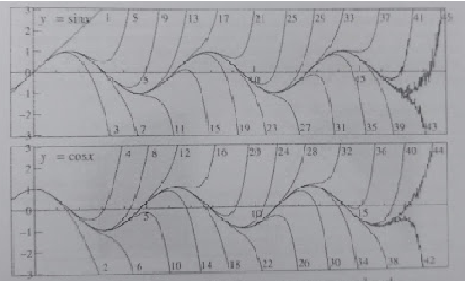
\includegraphics[width=0.60\linewidth]{graftrig.png}
\end{figure}
 

\newpage
\subsection{Sucesiones infinitas y Series infinitas} 

Con el objeto de justificar razonamientos utilizados en secciones anteriores, finalizaremos el Precálculo estudiando Sucesiones, Convergencia de una Sucesión, Series Infinitas y Convergencia de Series (Pág 172, 173, 188 de Analysis by Its History). Por tal motivo debemos introducir previamente la función módulo y el concepto de distancia. Tendremos que explicar qué significa matemáticamente el concepto $"$arbitrariamente cerca", para "$n$ suficientemente grande", etc.

%Ejemplos de sucesiones son una "progresión aritmética" (la diferencia entre dos términos sucesivos es constante), como $$\{1,2,3,4,...\},$$ una "progresión geométrica" (el cociente entre dos términos sucesivos es constante), como $$\{q^0,q^1,q^2,q^3,...\}.$$

En esta sección no vamos a reproducir la definición de sucesión, de límite de una sucesión (D'Alembert 1765, Cauchy 1821), definición de serie y convergencia de la misma, ya que son definiciones clásicas. Lo innovador es el hecho de que usualmente se introduce la definición de límite para funciones, continuidad, y como consecuencia obtenemos la definición de convergencia para sucesiones y series. Proponemos empezar el camino al revés, es decir, definir el límite de una sucesión (o sumas parciales en el caso de series) y manipular dicha definición para probar existencia y no existencia de dicho límite. Después en el cuatrimestre siguiente definir el concepto de función continua (es decir la definición de límite cuando el límite es una imagen de la función), y finalmente la definición de límite para una función real no necesariamente continua. Lo que se pretende al seguir este camino es lograr manipular estas definiciones antes de buscar otros caminos como criterios o teoremas que nos faciliten los cálculos.




\subsection{Prerequisitos, curso ingreso}

Para finalizar  queríamos referirnos brevemente a algunos prerequisitos de precálculo que consideramos importantes y son tratados normalmente en la escuela media, pero que juzgamos  pertienente retomar en el curso de ingreso a modo de artículación entre de los dos niveles educativos.  

Proponemos comenzar con un repaso del concepto de función, dominio, imagen, gráfico, inyectividad, suryectividad y funciones inversas (biyectividad). Todo esto podrá retomarse en cada subsección que veremos a continuación. Por ejemplo, se plantea estudiar función lineal y cuadrática a partir de bibliografía que puede ser utilizada en el nivel medio, con ejemplos fáciles de trabajar, y para cada una se estudiará sus gráficos, propiedades, inversas, etc. 

\subsection{Función lineal}

Comencemos con un interrogante... ¿Qué problemas modelizan una función lineal?

\begin{enumerate}
	
	\item [a)] Una empresa de taxi de la ciudad, cobra la bajada de bandera (costo fijo) a \$\ 50 y luego \$\ 2,50 por cada kilómetro recorrido. La relacion que modeliza el dinero gastado en función de los kilómetros recorridos $\textbf{Dinero=50+2,5.kilómetros}$ es una función lineal.
	
	\item [b)] El agua ocupa el 71 \%\ de la superficie del planeta. Sin embargo, es necesario comprender que no toda el agua es adecuada para el consumo humano. Sólo el 0,8 \%\ de su volumen es aprovechable por los seres humanos. El agua que puede beber
	el hombre proviene de reservas naturales de agua dulce (como los lagos, ríos y lagunas), reservas artificiales (diques y azudes) y acuíferos subterráneos. La creciente escasez de aguas lleva a que la sociedad debe concientizarse con su uso y cuidado.
	Si observamos la parte central de la factura de agua que la empresa proveedora del servicio envía a nuestro domicilio, por la provisión del agua potable cada mes, encontraremos los siguientes conceptos:
	\begin{figure}[h!]
		\centering				                     	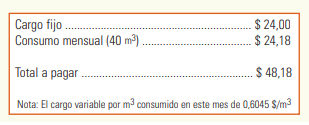
\includegraphics[width=0.70\linewidth]{facturaagua.png}
	\end{figure}
	En la factura leemos primero un cargo fijo de \$\ 24,00, aunque no usemos agua en el período facturado. Seguidamente, se informa la cantidad de $m^{3}$ que consumimos en nuestro domicilio este mes, 40 $m^{3}$, y en la nota indican el precio por cada $m^{3}$ de agua consumido (\$\ 0,6045 en este caso).
	A partir de estos datos, podemos construir una función $\textbf{Costo=24 + 0,6045.$m^{3}$}$, la cual muestra el costo aproximado en \$\ en función del consumo de agua. 
	
	\item [c)] Juan se está por tirar de un paracaídas y viaja en un avión que está a 10 km de altura. Si el paracaidista cae a 20km/h,  la ecuación que relaciona el tiempo de caída (en  minutos) con la altura en la que se encuentra Juan $\textbf{Altura= 10 - $\frac{1}{3}$. tiempo}$, es una función lineal.
	
	\item [d)] Marina tenía \$\ 4500 ahorrados, y le informaron del colegio que debía poner para el egreso \$\ 150 por mes para el egreso de fin de secundario. El modelo que relaciona el dinero que tiene Marina con el tiempo (en meses) $\textbf{Dinero= 4500 - 150. tiempo}$, es una función lineal.En este caso, el gráfico que resulta es:
\end{enumerate}

Los gráficos de estas funciones son los siguientes:


\begin{figure}[!h]
	\begin{center}
% 		\subfigure[]{\includegraphics[width=.4\linewidth,height=0.15\textheight]{grafico1.png}}
% 		\subfigure[]{\includegraphics[width=.4\linewidth,height=0.15\textheight]{grafico2.png}}
% 		\subfigure[]{\includegraphics[width=.4\linewidth]{grafica3.png}}
% 		\subfigure[]{\includegraphics[width=.4\linewidth,height=0.15\textheight]{grafica4.png}}
	\end{center}
\end{figure}

Como se observa, la función que modeliza estas situaciones es de la forma $y=a.x+b$, donde \textit{b} indica la oredenada al origen y el parámetro \textit{a} llamado \textbf{pendiente} nos dice si la función cuyo gráfico siempre resulta una recta, es creciente, decreciente o constante: 
\begin{itemize}
	\item Si \textit{a} es positivo, la recta es creciente.
	\item Si \textit{a} es negativo, la recta es decreciente.
	\item Si \textit{a} es cero, la recta resulta constante.
\end{itemize}

Además, si se analiza en profundidad por ejemplo la función del inciso c):

\begin{figure}[h!]
\centering
   %\includegraphics[width=0.4\linewidth]{grafica5.png}
  \caption{Mi Figura}
  
\end{figure}



Se puede observar que para cualquier par de puntos que pertenecen a la recta $(x_1,y_1), (x_2,y_2)$ se cumple que la pendiente resulta de hacer el cociente $\frac{y_1-y_2}{x_1-x_2}$\\

\vspace{3cm}

\textbf{Todas las rectas que se pueden dibujar en un plano coordenado,¿representan una función lineal?}
La respuesta es no. Si observamos la línea recta vertical que se muestra en el siguiente gráfico , vemos que todos los
pares ordenados que pertenecen a la misma son de la
forma $(2;y)$, donde la segunda coordenada y es un número real.
Observemos que para un valor fijo de x = 2, pertenecen al grafico los pares ordenados $(2;0),(2;2),(2;4),(2;-1)$ ,etc.,entonces esta recta NO representa una función.


%\begin{figure}[!h]
%	\begin{center}
%		\includegraphics[width=0.4\linewidth]{grafica6.png}
%	\end{center}
%\end{figure}













\subsection{Función Cuadrática}

Ahora pensemos en problemas que se modelizan con una función cuadrática...

Se dispone de 40 m de alambre para rodear un cantero rectangular en el que se va a realizar una plantación de rosales en un parque público. ¿Cuáles deben ser las dimensiones del cantero para que la superficie con césped resulte la máxima posible?

Observemos primero que existen muchos rectángulos cuyo perímetro es de 40 metros, a modo de ejemplo:\\
* Se puede tener un rectángulo de 1m x 19m, en este caso la superficie es de 19 $m^{2}$\\
* Tambien se puede tener un rectángulo de 5m x 15m, y la superficie del mismo es de 75 $m^{2}$.

\begin{figure}[h!]
\centering
	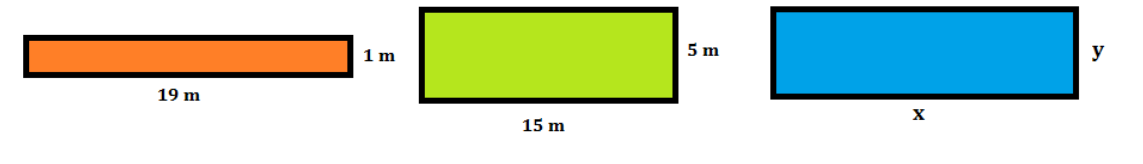
\includegraphics[width=0.90\linewidth]{rectangulos.png}
\end{figure}

Nuestro objetivo es encontrar las dimensiones del cantero, es decir la medida del largo (x) y ancho (y), que pueda contener la mayor superficie posible, a fin de plantar una cantidad considerable de rosales.
se conoce que la superficie es $S = x.y$ y además el perímetro es 40m, es decir $2.x + 2.y=40 $. De aquí se obtiene que $S= x.(20-x)$, con lo que finalmente, se puede escribir $S(x) = 20.x-x^{2}$

Con este modelo: 
\begin{itemize}
	\item Si el largo del cantero es $x = 19m$ , calculando la imagen de la función obtenemos: $S(19) = 20.19 - 192 \Rightarrow 
	S(19) = 19$.\\
	\item Si el largo del cantero es $x = 5m$ tendríamos:
	$S (5) =  20.5 - 25 \Rightarrow S (5) = 75m^{2}$.
	En este caso el cantero tendría menor superficie: $75 m^{2}$.
	Entonces, la superficie del cantero será de 19 $m^{2}$ (también coincide con lo que calculamos para el cantero que diagramamos antes).
\end{itemize}

Obviamente, es imposible seguir probando con todos los posibles largos del cantero para ver la superficie, pero podemos observar aquí que para esta función S la variable x (largo del cantero) aparece con exponente dos o potencia cuadrática, entonces, no es una función lineal del tipo de las que ya estudiamos.
En las funciones mediante las cuales se representan muchas situaciones y fenómenos cotidianos aparece, como en el problema anterior, la variable independiente (x) elevada a una potencia cuadrática, se denominan FUNCIONES CUADRÁTICAS.

Retomemos el problema del Ejemplo:
Se dispone de 40 m de alambre para rodear un cantero rectangular donde se va a realizar la plantación de rosales en un parque público. \textit{¿Cuáles deben ser las dimensiones del cantero para que la superficie con césped resulte la máxima posible?}\\
Si construimos una tabla que nos muestre la superficie del cantero en función de algunos valores del largo del mismo, a partir de la función cuadrática $S(x) =20x-x^{2}$, obtenemos:
% Please add the following required packages to your document preamble:
% \usepackage[table,xcdraw]{xcolor}
% If you use beamer only pass "xcolor=table" option, i.e. \documentclass[xcolor=table]{beamer}

%\begin{table}[!h]
%	\centering
%	\begin{tabular}{|
%			>{\columncolor[HTML]{FFCE93}}l |l|l|l|l|l|l|l|}
%		\hline
%		Largo del cantero x (m)                         & 0 & 5  & 8  & 10  & 14 & 17 & 20 \\ \hline
%		Superficie S del cantero ($m^{2}$) & 0 & 75 & 96 & 100 & 84 & 51 & 0  \\ \hline
%	\end{tabular}
%\end{table}

Observación: Cuando los valores del largo son de 0 m y 20 m el área de la región ocupada es de 0 $m^2$ ya que en ese caso no estaríamos conformando ningún rectángulo, sólo sería una línea de 40 m de alambre.
Si ubicamos en un sistema de coordenadas los pares ordenados $(x,y)$ que verifican esta
función cuadrática S, y adicionamos algunos más para ayudarnos a determinar la forma, obtenemos el siguiente gráfico:

\begin{figure}[h!]
	\centering
	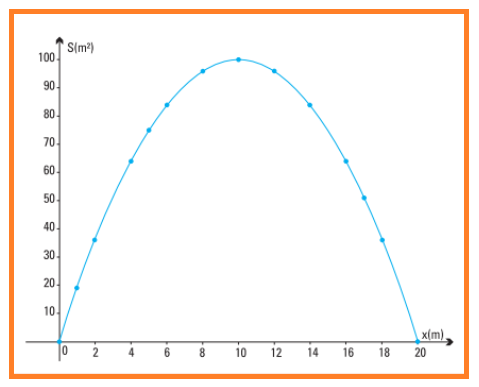
\includegraphics[width=0.45\linewidth]{cuadratica1.png}
\end{figure}

Como cualquier valor de número real entre 0 y 20 sería posible para el largo del cantero, es correcto conectar los puntos con una curva continua, todos los puntos de esta función cuadrática pertenecen a la curva que se denomina \textbf{Parábola}.

Parece que la gráfica alcanza su máximo valor en el par ordenado $(10,100)$, que indica que el cantero con un largo de 10 m tiene el área mayor, 100 $m^2$.

El punto donde la parábola alcanza su máximo valor se denomina \textbf{Vértice}.

En general, las ecuaciones de las funciones cuadráticas "tienen la forma":
\begin{center}
	\textbf{$f(x)=a.x^{2}+b.x+c$}
\end{center}

Observación: En el ejemplo analizado, $a=-1, b=20$ y $c=0$.

Cada uno de los parámetros involucrados en la ecuación proveen información importante sobre la función cuadrática.

Por ejemplo, si se estudia la función es $y = a.x^{2}$, para distintos valores de \textit{a}, se obtienen los siguientes gráficos:

\begin{figure}[h!]
	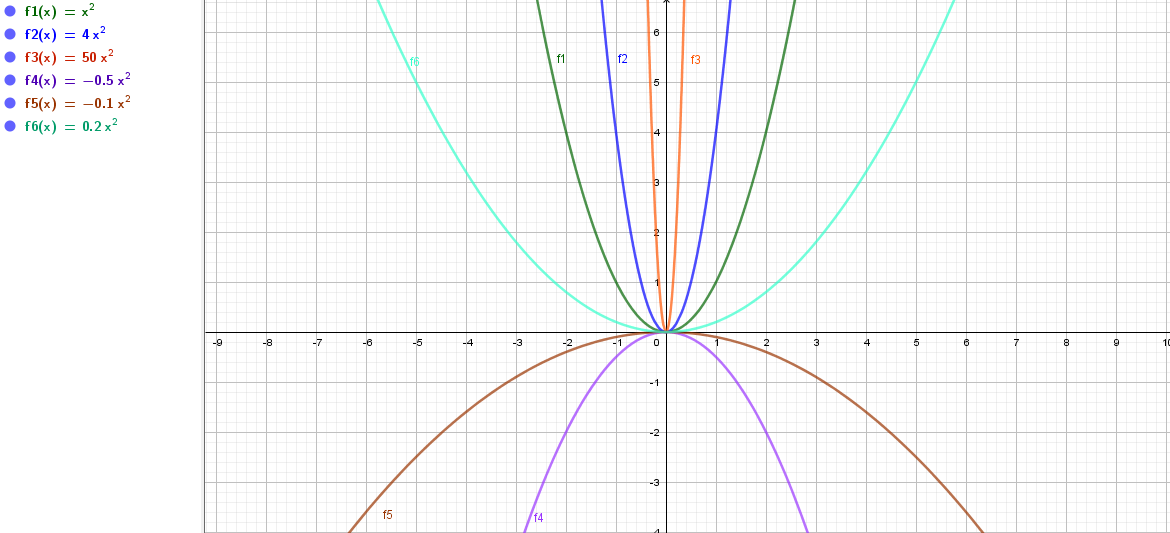
\includegraphics[width=0.9\linewidth]{cuadratica3.png}
\end{figure}

Así se observa que si $\textit{a} > 0$
\begin{itemize}
	\item Tiene ramas hacia arriba
	\item Alcanza su valor mínimo en el vértice
	\item El eje de simetría es el eje y
	\item Cuanto mayor sea el valor del parámetro \textit{a} más cerrada será la parábola
\end{itemize} 
Si  $\textit{a} < 0$
\begin{itemize}
	\item Tiene ramas hacia abajo
	\item Alcanza su valor máximo en el vértice
	\item El eje de simetría es el eje y
	\item  Cuanto mayor sea el valor absoluto del parámetro \textit{a} más cerrada será la parábola
\end{itemize} 


 \section{Propuesta para Algebra I } 
 
 

\subsection{Introducción y fundamentación}

 

Se abordarán dos tipos de pensamiento

\begin{itemize}
\item El pensamiento aritmético a través del estudio de estructuras algebraicas como conjuntos de números con su aritmética específica y anillos de polinomios.
\item El pensamiento combinatorio a través de problemas de conteo. 
\end{itemize}


Se presentan la teoría de conjuntos y la lógica proposicional como introducción a la práctica de la fundamentación matemática. 

Los números naturales aportan un procedimiento de validación simultánea 




\textcolor[rgb]{1,0,0}{En construcción}





\subsection{Algunos Problemas }

\subsubsection{Combinatoria}

 
\noindent  \textit{\textbf{Problema 1.    El principio del palomar }} 


Sean $n$ y $k$ dos enteros positivos y sea $n>k$. Supongamos que queremos ubicar $n$ bolas idénticas en $k$ cajas idénticas. Entonces hay al menos una caja en la cual ubicaremos al menos dos bolas.

Solución: asumamos que por el absurdo no hay ninguna caja con al menos dos bolas. Entonces cada una de las $k$ cajas tiene o una o ninguna bola. Sea $m$ el número de cajas que tienen cero bolas en ellas (el número de cajas vacías). Luego, hay $k-m$ bolas que tienen una bola. Pero entonces hay un total de $k-m$ bolas ubicadas en las $k$ cajas, lo que es un absurdo.


\bigskip
\noindent  \textit{\textbf{Ejercicio}}. 

Hay al menos un elemento de la secuencia $7,77,777,7777,\ldots$ que es divisible por $2003$.





\subsection{Contenidos }


\subsubsection{Nociones de lógica}
%Sanchez
\begin{itemize}
	\item Lógica proposicional. Proposiciones. Conectivos lógicos. Fórmulas proposicionales. Razonamientos. Funciones proposicionales. 
	
	\item Lógica matemática. El método matemático. 
	
	%\item  Cuantificadores: noción intuitiva.
\end{itemize} 

\subsubsection{Conjuntos, relaciones y funciones}

\begin{itemize}
\item Conjuntos: definición intuitiva, operaciones entre conjuntos.   Cardinal de conjuntos finitos.  El conjunto potencia o conjunto de partes. 

\item Relaciones: definición, su representación como grafos.  Relaciones de orden y su representación por medio de Diagramas de Hasse.  Elementos minimales, maximales, conjuntos acotados. Primer y último elemento. Relaciones de equivalencia. Clases de equivalencia.  Clausura transitiva.

\item Funciones: definición. Composición. Funciones inyectivas, sobreyectivas, biyectiva, inversa.

%\item  Cuantificadores: noción intuitiva.
\end{itemize} 
 
\subsubsection{Números naturales e Inducción}

\begin{itemize}
\item Conjuntos inductivos. Definición del conjunto de números naturales $\mathbb{N}$. Principales propiedades. 
\item Sumatoria, productoria y su escritura como ciclos en un programa. Factorial y su interpretación combinatoria (biyecciones en conjuntos finitos). 
\item Número combinatorio y su interpretación combinatoria (subconjuntos en un conjunto finito), escritura como suma de dos combinatorios, definición recursiva del combinatorio. 
\item  Definición de funciones recursivas en pseudocódigo (o código en algún lenguaje concreto). 
\item Definición por los axiomas de Peano de los números naturales. 
\item Ejemplos de demostración por inducción global. 
\item  Ejemplos de algoritmos recursivos (sort, Hanoi, Fibonacci) y análisis de complejidad. Cálculo de $a^n$ por distintos algoritmos (introducción intuitiva de noción de complejidad). Inducción global y principio de buena ordenación.
 \end{itemize}


\subsubsection{Números enteros}

 \begin{itemize}
 \item  Ejemplos de algoritmos recursivos (sort, Hanoi, Fibonacci) y análisis de complejidad. Cálculo de $a^n$ por distintos algoritmos (introducción intuitiva de noción de complejidad). Inducción global y principio de buena ordenación.

 \item Enteros. Divisibilidad y primeras propiedades. Primos y Compuestos.  Algoritmo de división. Aplicaciones del algoritmo de división. Escrituras en distintas bases, sistemas de numeración.  Máximo común divisor.  Algoritmo de Euclides (y su complejidad), escritura del máximo común divisor como combinación lineal. Numeros coprimos. Propiedades. Teorema Fundamental de la aritmética (TFA). Cantidad de primos. Criba. Aplicaciones del TFA (cantidad de divisores, cálculo de gcd y del mcm). Curiosidades de los primos. Congruencias,  propiedades y aplicaciones (criterios de divisibilidad). Restos modulo m. Grupos y Anillos (comparación de $\mathbb{Z}/m\mathbb{Z}$). 

 \item Ecuaciones lineales diofánticas y ecuaciones de congruencia. Algoritmos. Sistemas de ecuaciones de congruencia. Teorema Chino del Resto. Pequeño Teorema de Fermat. Algoritmos probabilisticos de primalidad. de Euler-Fermat. Aplicación: Algoritmo criptográfico RSA.
  \end{itemize}


\subsubsection{Combinatoria}
 El principio del palomar. Combinatoria enumerativa. Conteo. Teorema binomial, multinomial e identidades relacionadas.


\subsubsection{Polinomios con coeficientes en un cuerpo}

 \begin{itemize}
 \item  Cuerpos. Definición y ejemplos, $\mathbb{Q}, \mathbb{R}, \mathbb{C}, \mathbb{Z}/p\mathbb{Z}$. Anillo de polinomios K[x]: generalidades (suma, producto, unidades), grado, divisibilidad, irreducibles y compuestos,  algoritmo de división. Paralelismo con Z: Máximo común divisor, algoritmo de Euclides, coprimos. Factorización única. 

 \item Aspecto funcional: Evaluacion de polinomios (def y algoritmos). Raíces. Teorema del resto. Resolución de cuadraticas en $K[X]$. Multiplicidad. Equivalencias. Cota para el número de raíces con multiplicidad sobre un cuerpo.

 \item $\mathbb{C}[X]$: Repaso del cuerpo $\mathbb{C}$, coordenadas polares, fórmulas de Moivre.  Grupo de raíces de la unidad. Teorema Fundamental del Algebra, irreducibles de $\mathbb{C}[X]$.  

 \item $\mathbb{R}[X]$: Raíces complejas no reales de polinomios reales.  Factorización en $\mathbb{R}[X]$.

 \item $\mathbb{Q}[X]$: Teorema de Gauss para calcular raíces racionales.

 \item Ejemplos de factorización en $K[X]$ para distintos $K$. Criterios de irreducibilidad sobre Q y algoritmos de factorización sobre los distintos cuerpos
 \end{itemize}

 
Ver http://cms.dm.uba.ar/academico/programas/algebraI


\section{Geometría}

\subsection{Situación actual}

\subsubsection{Contenidos mínimos propuestos por el plan de estudios 2008 versión 2}

Triángulos medianas, mediatrices, centroides. Inscriptos y
circunscriptos. Ortocentro. Polígonos: simetrías. Isometrías del
plano euclídeo. Geometría afín: ecuaciones de rectas  en
el plano y de rectas y planos en el espacio. Espacios vectoriales generales.
Transformaciones lineales: rotaciones, reflexiones, simetrías.
Cónicas y cuádricas.

\subsubsection{Contenidos programa vigente}

\begin{description}
 \item[Unidad 1. Angulos y Rectas]
Axiomas de medición de ángulos y de medición de segmentos. Ángulos
adyacentes y opuestos por el vértice. Bisectriz de un ángulo. Angulo recto.
Rectas perpendiculares. Rectas paralelas. Construcciones con regla y
compás. Ángulos determinados por dos rectas y una transversal.

 \item[Unidad 2. Triángulos y Cuadriláteros]
Congruencia de triángulos. Criterios. Relaciones entre lados y ángulos de
un triángulo.
Alturas, medianas y bisectrices de un triángulo. Elementos notables de un
triángulo.
Cuadriláteros convexos. Paralelogramo, rectángulo, rombo, trapecio.
Propiedades.

 \item[Unidad 3. Isometrías]
Concepto de movimiento. Propiedades de los movimientos. Rotaciones,
traslaciones, simetrías (central y axial).

 \item[Unidad 4. Circunferencia]
Definiciones básicas. Tangente a una circunferencia. Ángulo central,
ángulo inscripto, ángulo semiinscripto: propiedades.

 \item[Unidad 5. Semejanza de triángulos]
Teorema de Thales. Teorema de Thales en el triángulo. Semejanza de
triángulos. Criterios. Teorema de Pitágoras

 \item[Unidad 6. Vectores.] Rectas y Planos en el espacio tridimensional
Vectores. Definición geométrica y algebraica. Operaciones. Norma de un
vector. Producto escalar. Ecuaciones de rectas (vectorial, paramétrica,
simétrica) y planos (implícita, punto-normal) Posiciones relativas entre
rectas, planos, planos y rectas

\item[Unidad 7. Cónicas]
Parábola, elipse e hipérbola: definición como lugar geométrico, ecuación
canónica, elementos distinguidos, propiedades. Traslación de
coordenadas.
\end{description}

\subsubsection{Observaciones.} El programa de la materia cubre los temas propuestos en el plan de estudios. Sin embargo se considera que las horas dedicadas a la unidad temática Geometría Analítica son insuficientes para la nueva propuesta de Plan de Estudios en la Lic en Matemática. Se propone fortalecer la foermación en  \emph{Geometría Analítica}.  





\subsection{Propuesta de innovación} Se propone desdoblar la asignatura actual en dos asignaturas a desarrollarse en el primer año de la cursada. Una de ellas dirigida a lo que denominaremos \emph{Geometría Sintética} y la otra \emph{Geometría Analítica}. Lo que distingue una de otra es la utilización de coordenadas. 

\subsubsection{Geometría sintética} 
\subsubsection{Objetivos} 

Adherimos a los expresados en el programa vigente
\begin{itemize}
 \item Desarrollar procederes propios de las ciencias axiomático deductivas.
 \item  Percibir el carácter funcional de las propiedades de los objetos
geométricos
 \end{itemize}

Se propone incorporar los siguientes objetivos.

\begin{itemize}
  \item Desarrollar estrategias para resolver problemas.
  \item Desarrollar el concepto de área de regiones elementales, por ejemplo triángulos y rectángulos. Es importante notar que el concepto de área se empieza a desarrollar en la asignatura Cálculo I dando ya por sentado las fórmulas de área de las figuras elementales.
  \item Incorporar temas un poco más elaborados dentro de la geometría sintética, por citar ejemplos Teoremas de Ceva, Napoleón, 9 puntos, Morley, etc, ver por ejemplo ejemplo \cite{O.Bottema149,H.S.M.Coxeter35,H.S.M.Coxeter226,RogerFenn248,AllanBerele41}.
  \item Como idea tentativa, usar Geogebra activamente en clases \cite{GerardA.Venema145}.
\end{itemize}


\subsubsection{Contenidos mínimos.} Axiomas de Euclides. Triángulos. Construcción con regla y compás. Altura, mediana y mediatrices. Congruencia y semejanza. Elementos notables y sus relaciones.  Polígonos. Cuadriláteros convexos. Polígonos regulares. Circunferencia.
 Propiedades de rectas, segmentos y ángulos en una circunferencia. Polígonos inscriptos y circunscriptos. Construcción con regla y compás. Rectas y Planos. Intersecciones en el plano y el espacio (desde el punto de vista axiomático). Postulados de rectas paralelas: condiciones suficientes para el paralelismo. Teorema de Thales. Teoremas de semejanzas. Segmento. Congruencia y comparación (desde el punto de vista axiomático).Teoremas de Ceva, Napoleón, 9 puntos y Morley. Área de regiones planas elementales. 
 
\subsubsection{Bibliografía consultada.} Libros que mejor se adapatan a la propuesta\linebreak \cite{AllanBerele41},\cite{RogerFenn248},\cite{RobinHartshorne131},\cite{AlfredS.Posamentier49}. Profundización en la teoría \cite{O.Bottema149,CharlesStanleyOgilvy129}. Para trabajar la noción de  área \cite{AllanBerele41}. Colecciones de problemas \cite{M.N.Aref52,EvanChen132}, Axiomática \cite{GerardA.Venema145}\linebreak\cite{RobinHartshorne131}. Geogebra \cite{GerardA.Venema145}. Consulta \cite{H.S.M.Coxeter226,H.S.M.Coxeter35,MatthewHarvey261,RogerA.Johnson42}.



\subsubsection{Geometría analítica} 
\subsubsection{Objetivos} 
Como señala el programa vigente
\begin{itemize}
  \item  Reconocer la complementariedad entre las geometrías analítica y
sintética
\end{itemize}

Sugerimos considerar los siguientes objetivos
\begin{itemize}
  \item Desarrollar estrategias para resolver problemas.
  \item Desarrollar la capacidad de representar algebraicamente lugares geométricos y curvas definidas de manera dinámica.
  \item Reconocer la importancia del concepto de transfomación, particularmente rígidas, homotecias y afines. Puede  considerarse transformaciones proyectivas. 
  \item Fomentar la capacidad para reducir ecuaciones por medio de distintos grupos de transformaciones.
  \item Incorporar el uso de herramientas computacionales. 
\end{itemize}

\subsubsection{Contenidos mínimos.}  Transformaciones en el plano. Isométricas: Reflexiones. Traslaciones. Rotaciones.  No isométricas: Homotecias. Transformaciones afines.  Inversión respecto de una cicunferencia. Vectores. Producto interno y exterior.   Ecuaciones paramétrica e implícita de  recta y planos. Demostración de algunos resultados de geometría euclideana por medio de geometría analítica. Cónicas. Definición como lugar geométrico. Ecuaciones paramétricas e implícitas. Ecuación general de segundo grado y su reducción por transformaciones rígidas o afines. Propiedades notables, por citar ejemplo reflexión dentro de elipses, etc. Cuádricas. 

\subsubsection{Bibliografía consultada.} Libros que se adapatan a la propuesta \cite{C.G.Gibson97,RogerFenn248,DavidABrannan247,GeorgeA.Jennings273,DanPedoe81}. Cónicas \cite{ArsenyV.Akopyan95,VagnLundsgaardHansen85}, Grupos transformaciones \cite{H.S.M.Coxeter226, IlkaAgricola77,JudithCederberg101}, Uso de software \cite{DonaldL.Vossler72}, Historia \cite{JulianLowellCoolidge74},Consulta \cite{H.S.M.Coxeter226, IlkaAgricola77,MicheleAudin38,V.V.Prasolov88}. 
 
 
\subsection{Mapa conceptual Geometrías Elementales}

\begin{center}
 



\begin{tikzpicture}[thick,scale=0.6, every node/.style={scale=0.6}]
  \path [
  %%Configuración
    mindmap,
    text = black,
      level 1 concept/.append style =
      {font=\small\bfseries, sibling angle=72,minimum size=2.5cm,level distance=15em},
    level 2 concept/.append style =
      {font=\normalsize\bfseries,level distance=10em,minimum size=2cm, sibling angle=40},
    level 3 concept/.append style =
      {font=\scriptsize,level distance=5em,minimum size=1cm,sibling angle=45},
    tex/.style     = {concept , ball color=green!20!black,
      font=\Large\bfseries},
    engines/.style = {concept, ball color=green!50!black},
    formats/.style = {concept, ball color=blue!50!black},
    systems/.style = {concept, ball color=red!90!black},
    editors/.style = {concept, ball color=green!100!black},%= {concept, ball color=orange!50!black}
    2cuerpos/.style = {concept, ball color=yellow!90!black}
  ]
    %%Nodos
  node [tex] {Geometría\\Elemental} [concept  color=green!20!black,clockwise from=0]
    child [concept color=green!50!black, nodes={engines}] {
      node {Sintética} [clockwise from=80]
          child [concept color=green!100!black, nodes={editors}] {
		node {Congruencia} [clockwise from=0]}
	  child [concept color=green!100!black, nodes={editors}] {
		node {Similaridad} [clockwise from=0]}
          child [concept color=green!100!black, nodes={editors}] {
		node {Incidencia} [clockwise from=0]}
	  child [concept color=green!100!black, nodes={editors}] {
		node {Polítopos} [clockwise from=0]}
	  child [concept color=green!100!black, nodes={editors}] {
		node {Circunsferencia} [clockwise from=0]}
}
    child [concept color=green!50!black, nodes={engines}] {
      node {Grupos\\Transformaciones} [clockwise from=-20]
	   child [concept color=green!100!black, nodes={editors}] {
		node {Afín} }
	  child [concept color=green!100!black, nodes={editors}] {
		node {Rígidas} }
	child [concept color=green!100!black, nodes={editors}] {
		node {Proyectivas} }
    child [concept color=green!100!black, nodes={editors}] {
		node {Inversión} }
		}
        child [concept color=green!50!black, nodes={engines}] {
      node {Proyectiva}[clockwise from=234]
	   child [concept color=green!100!black, nodes={editors}] {
		node {Plano\\Proyectivo}}
		child [concept color=green!100!black, nodes={editors}] {
		node {Cónicas} } 
	}
    child [concept color=green!50!black, nodes={engines}] {
      node {Analítica} [clockwise from=234]
	   child [concept color=green!100!black, nodes={editors}] {
		node {Vectores}}
	  child [concept color=green!100!black, nodes={editors}] {
		node {Ecuaciones\\Paramétricas\\Implícitas} }
	child [concept color=green!100!black, nodes={editors}] {
		node {Rectas\\Planos} }
	child [concept color=green!100!black, nodes={editors}] {
		node {Cónicas} }
    	child [concept color=green!100!black, nodes={editors}] {
		node {Otras\\Curvas} }
	}
    child [concept color=green!50!black, nodes={engines}] {
      node {No Euclideana}  [clockwise from=92]
	   child [concept color=green!100!black, nodes={editors}] {
		node {Hiperbólica}}
	  child [concept color=green!100!black, nodes={editors}] {
		node {Esférica} }
      }

;
\end{tikzpicture}


\end{center}



 



\section{Modelización}



\begin{enumerate}
 \item \textbf{OBJETIVOS PROPUESTOS}
      %\begin{description}
      Se aspira que el alumno alcance los siguientes objetivos.

      \begin{enumerate}
      
        \item\label{it:1} Que integre los conocimientos adquiridos  durante el curso de su carrera en un marco conceptual ligado a las aplicaciones y al modelado matemático.

        
	\item\label{it:2} Se apropie de lenguajes, métodos y conocimientos de otras disciplinas científicas.

           \item\label{it:3} Mejore su capacidad para comunicarse con otros profesionales no matemáticos y brindarles asesoría en la aplicación de la matemática en sus respectivas áreas de trabajo.

           \item\label{it:4} Se capacite en la habilidad de extraer información cualitava de datos cuantitativos.

           \item\label{it:5} Desarrolle la capacidad de utilizar las herramientas computacionales de cálculo numérico y simbólico para plantear y resolver problemas.
 
	    \item\label{it:6} Logre la capacidad  de construir  modelos matemáticos a partir de situaciones reales.

     
           \item\label{it:8} Se adiestre en la utilización de  métodos analíticos para el análisis de modelos matemáticos y de allí establecer conclusiones sobre la realidad que ellos representan.
           
    
        

          \end{enumerate}


\item \textbf{CARACTERÍSTICAS DE LA MATERIA}

\begin{description}
\item[Curricula Flexible.]  
		Hay una gran variedad de técnicas, métodos y teorías matemáticas que son utilizadas para desarrollar modelos matemáticos: Teoría de Optimización, Teoría de Control, Ecuaciones Diferenciales Ordinarias, Ecuaciones Diferenciales Parciales, Ecuaciones con retardo, Ecuaciones en diferencias, Procesos Estocásticos, Autómatas, Teoría de Juegos, etc. A su vez la modelación matemática se aplica a una gran variedad de contextos: economía, biología, sociología, medicina,  dinámica de los lenguajes, física, deporte, etc. 
		
		Una característica propia de los modelos matemáticos es que sucesos del devenir natural y humano hacen que algunos temas relacionados con la modelación  adquieran repentina e impactante relevancia. Un ejemplo superlativo de ello es la pandemia del COVID-19. 
		
		Debido a la diversidad mencionada de temáticas y a las dinámicas   cambiantes de las mismas se piensa que la mejor alternativa es proponer que la materia sea un espacio abierto, donde los docentes responsables del dictado, guiados por las  consideraciones expuestas en este documento, elaboren un programa para la asignatura. La CCP de la Lic. en Matemática se encargará de efectuar una revisión periódica a fin de evaluar que las actividades propuestas se ajusten en cantidad, calidad y orientación con las exigencias del plan. Esta tarea se llevará adelante cada vez que haya un cambio del plantel docente y  con una periodicidad no inferior a dos años.  
  
  \item[Situaciones problemáticas reales.] Es aconsejable que el alumno se enfrente durante el cursado con situaciones problemáticas de una complejidad comparable a la que se le presentaría en la realidad y no sólo exponerlo a modelos simplicados. Se debe tender a que el estudiante desarrolle la capacidad de determinar qué técnicas y teorías matemáticas son las más adecuadas para modelizar esa realidad.  Por consiguiente la materia debe formar al alumno en el manejo de una variedad representativa de estas técnicas.
  
  \item[Computación científica.]  Esto contempla la solución por medio de recursos computacionales de problemas matemáticos, la simulación de sistemas determinísticos evolutivos o la estimación de probabilidades de escenarios posibles en modelos estocásticos.  Es aconsejable tanto el uso de la computadora para resolver problemas  numéricamente, como valerse de sistemas de algebra computacional (SymPy, Mupad, Mathematica, Maple, etc) para la solución de problemas analíticos. 
  
  \item[Eficiencia] Un objetivo  de la materia es desarrollar la capacidad de resolver problemas. La evaluación de la consecución de este objetivo debe ser ponderada tanto en la complejidad de los problemas abordados, como en el tiempo empleado en ello. En ese sentido es recomendable que el alumno aprende de valerse de recursos que ya están disponibles para resolver estos problemas. Por ejemplo, en la actualidad muchos lenguajes de computación ofrecen multitud de librerías, desarrolladas por usuarios de todo el mundo, especializadas en resolver problemas de distintas áreas de la matemática.  La materia debe capacitar en buscar estos recursos, aprender a utilizarlos de manera autónoma. 
  
  
  \item[Interdisciplinaridad] Es aconsejable que durante el cursado invite a especialistas de otras áreas del saber a ofrecer charlas en el marco de la materia sobre problemáticas relacionadas con la modelización matemática. Deberían proponerse mecanismos de certificación y reconocimiento de estas actividades para los especialistas intervinientes.
  
  \item[Intradisciplinaridad.] Propender a la consedireción de diversidad de teorías matemáticas, analizar los supuestos a los que mejor se ajustan cada una de ellas. Favorecer la participación de  docentes con inserción en las diferenctes líneas de investigación del departamento.  


\end{description}

  \item \textbf{Unidades temáticas y contenidos}

  La siguiente enumeración pretende ser amplia pero no exhaustiva. Fue elaborada con el criterio de que queden representados una variedad grande de técnicas matemáticas. Recopila las temáticas históricas abordadas en la asignatura. Es presentada a modo de guía para los docentes responsables del espacio curricular. \emph{Los mismos pueden confeccionar el programa eligiendo algunos temas de esta guía o proponer otros}. 
  
  
  

\begin{description}


\item[Generalidades]  Ingredientes de un modelo matemático. Variables, pará-
metros, ecuaciones de estado. Teorías, Leyes Generales y relaciones constitutivas. Va-
lidación de un modelo. Clasificación de los modelos: estáticos, dinámicos, determi-
nistas, estocásticos, discretos y continuos.  \cite{bellomo1994modelling,SandipBanerjee729,MattiHeilio730}.


\item[Análisis Dimensional] Cantidades y dimensiones.  Unidades primitivas y derivadas. El sistema internacional de unidades SI. Homogeneidad dimensional. Proceso de adimensionalización. El Teorema $\pi$-Buckingham. Aplicaciones
\cite{ThomasWitelski711,MattiHeilio730,MarkH.Holmes706,CliveDym710,EdwardA.Bender715,C.C.Lin720}


\item[Sistemas mecánicos] Sistemas de coordenadas inerciales. Mecánica Newtoniana. Ecuaciones de Newton. Leyes de balance. Vínculos. Principio del trabajo virtual. Sistemas conservativos. Ecuaciones de Lagrange. Multiplicadores de Lagrange y cálculo fuerzas de vínculo. Fricción seca y soluciones débiles de Fillippov. Elasticidad. Estudio cualitativo de sistemas. El péndulo y las integrales elípticas y las funciones elípticas de Jacobi. El problema de los dos cuerpos. Estudio cualitativo  de sistemas. Equilibrios. Soluciones homoclínicas y heteroclínicas. Cuerpo rígido. El grupo de Lie  $\SO(3,\mathbb{R})$ y el álgebra de Lie $\anti(n,\mathbb{R})$. Velocidad angular. Matriz de inercia. Ecuaciones de movimiento del cuerpo rígido. Estudio cualitativo del cuerpo aislado. \cite{CliveDym710,lemos2007mecanica,DavidBetounes488,goldstein1987mecanica,arnold2007mathematical,arnold2013mathematical, NicolaBellomo725} 

\item[Procesos de ramificación (branching)] Funciones generatrices de probabilidad: introducción y propiedades generales. Caracterización de las sucesiones de los tamaños $Z_n$ de la $n-$ésima generación. Probabilidades de extinción   del proceso $\{Z_n \}$. Modelos de crecimiento poblacional a edades dependiente (age-dependent branching processes).    Bibliografía:  \cite{grimmet2004, SandipBanerjee729,durrett2010probability,LindaJ.S.Allen616}. 

\item[Procesos de Markov.] Propiedades generales, funciones generatrices y clasificación de estados. Modelos de dinámicas poblacionales y evolución temporal del proceso de ramificación. Introducción a los procesos de nacimiento y al proceso de Poisson.   Bibliografía:  \cite{grimmet2004, SandipBanerjee729,durrett2010probability,LindaJ.S.Allen616}.


\item[Dinámica de poblaciones] Ecuaciones en diferencias. Ecuaciones lineales con coeficientes constantes. Independencia lineal. Casoratiano de funciones. Ecuación no homogénea. Método de coeficientes indeterminados. Sistemas de ecuaciones en diferencias lineales con coeficientes constantes. Algorítmo de Putzer. Matrices diagonalizables. Autovalores y autovectores. autovectores generalizados. Formas de Jordan.  Aplicaciones de ecuaciones escalares, modelos discretos de poblaciones de una
especie. Aplicaciones de sistemas de ecuaciones. Modelos estructurados. Modelos de
Leslie de estructuras por edad. Modelos de Usher. Otros tipos de modelos más generales. Teorema de Perron-Frobenius, digrafos asociados a matrices. Tests de positividad. Comportamiento en grandes escala de tiempo del modelo de Leslie. 
 Ecuaciones en diferencias no-lineales. Puntos fijos y soluciones periódicas. Estabilidad, estabilidad local y asintótica. Método de la teleraña. Estabilidad global. Teoría de bifurcaciones. Caos. Exponentes de Lyapunov. Modelos: Nicholson-Bailey, huesped parásito, predador-presa. Modelos continuos. Especies que interactúan. Competencia. Ecuaciones de Lotka-Volterra. Ecuaciones con retardo. Control óptimo. \cite{LindaJ.S.Allen747,SaberN.Elaydi423,RichardHaberman712,ElizabethS.Allman375, MartinBraun727,RichardHaberman712,YangKuang742,JamesD.Murray744,anita2011introduction}

\item[Modelos Epidemiológicos]  Modelos compartimentados. Influencia de la demografía. Modelos SIS, SIR y SEIR. El parámetro $\mathscr{R}_0$. La relación final. Equilibrios y extinsión. Modelos SIR y SIS estocásticos. Cadenas de Markov Discretas y continuas. Ecuaciones diferenciales estocásticas. Problemas de control óptimo. \cite{FredBrauer479,MaiaMartcheva480,FredBrauer,AllenSto,BerndBlasius746,OdoDiekmann614,JamesD.Murray745,JamesD.Murray744,anita2011introduction}.


\item[Dinámica medios continuos] Hipótesis de continuidad de la materia. Densidad. Cantidades intensivas y extensivas. Coordenadas Lagrangianas y Eulerianas. Derivadas magnitudes intensivas y extensivas. Teorema del Transporte de Reynolds.  Balance  de  masa. Fuerzas superficiales y extendidas. Teorema de Cauchy. Balance del momento lineal. Dinámica del Calor.  Calor específico. Energía. Unidades de medida.    Balance de energía. Fluidos incompresibles no viscosos.  Ecuaciones de Euler.  Fluidos incompresibles  viscosos. Tensor de deformaciones. Ecuaciones de Navier-Stokes. Ley de conducción de fourier. Ecuación del Calor. Ecuación de ondas. Modelos de tráfico vehicular.\cite{MarkH.Holmes706,JacekBanasiak709, MartinBraun727,bellomo1994modelling,AlexandreJ.Chorin749,FridtjovIrgens750,MichaelGriebel751,GiovanniP.Galdi752,PieterWesseling754,RichardHaberman712,C.C.Lin720}


\item[Modelos en medicina] Génesis tumoral. Modelos determinísticos. Modelos estocásticos.     \cite{DominikWodarz734,EmmanuelBarillot736,M.Eisen733,JamesD.Murray744,W.Y.Tan732}

\item[Optimización, ajuste paramétrico] \cite{EdwardA.Bender715,NeilA.Gershenfeld717,OdoDiekmann614,LyleD.Broemeling615}
El problema del estimación de parámetros  de modelos. Mínimos cuadrados. Método de Newton.  
Método de Levenberg—Marquardt. Estimación de máxima verosimilitud.  Aplicaciones a modelos
poblacionales, epidemiológicos, etc. 


\item[Modelos en el deporte] Coordenadas geográficas y proyecciones cartográficas. Topografía: imágenes geotiff. Matlab: lectura de archivos, interpolación de funciones, desarrollo de interfaces de usuario. Lenguajes  XML y GPX: breve descripción. Repaso de los conceptos de trabajo y potencia. Fuerzas que se oponen al movimiento de un ciclista. La ecuación del ciclista. \cite{wilson2004bicycling}

\item[Economía Matemática]  El equilibrio en los modelos económicos lineales. Un amplio esbozo de un flujo circular. Representaciones mediante ecuaciones lineales. La condicion de Hawkins-Simon. outputs y precios.  El teorema de Frobenius. Restricciones de no negatividad. El problema del valor propio no negativo. La raiz de Frobenius. Significado económico de la raiz de Frobenius. Series de Neumann. Matrices no descomponibles. Estabilidad relativa de la trayectoria de crecimiento equilibrado. \cite{Nikaido}.



\end{description}



  


\end{enumerate}


\section{Propuesta para Programaci\'on para Matem\'atica}

\noindent\textbf{Autor: Dr.\ Valent\'in Cassano}

tomadas de: How important is programming for mathematicians?

\href{https://math.stackexchange.com/questions/132042/how-important-is-programming-for-mathematicians}{https://math.stackexchange.com/questions/132042/how-important-is-programming-for-mathematicians}


 

\subsection{Introducción y fundamentación}

\cite{Seroul:2000,Rose:2015}



Razón principal:


\begin{itemize}
	\item Computers are right now are omnipresent, and efficient computer use = you know how to program and automate things.
\end{itemize}

De manera mas específica:

\begin{itemize}
	\item It is much easier to verify multiple cases using computer, e.g. the only known proof of the four color theorem is computer-assisted.
	
	\item Computer can solve (symbolically) many tedious things fast, things that would take you weeks or even months to calculate by hand, e.g. integration, many types of ODEs or PDEs, minimization problems, linear programming and extrema finding, even formula simplification.
	
	\item Every mathematical software (Maple, Matlab, Mathematica, but also Sage, Octave, and so on) are based on a programming language that you use to tell the program what you want to do.
	
	\item Many mathematical problems are too hard to solve symbolically, but often you can find numerical solutions with arbitrary precision.
	
	\item A number of math-related topics (or other domains that extensively use math nowadays, like computational biology, meteorology, financial analysis, quantum physics, ...) requires computers to work with.
	
	\item Using computer you can visualize your results to gain intuition, or to present it to a wider audience, etc. Knowledge of a programming language helps, e.g., with generating and transforming data.
	
	\item Automation! This is what computers are really good at, so if you need to preform some well defined tasks on large sets of data, just make computer do your work. This said, usually, in research, there are no tools that would do exactly what you want, just some building blocks of some sort, so you need to know how to use them and build even more awesome things.
	
	\item Finally, theoretical computer science is a part of mathematics (theoretical computer science $\neq$ informatics, I am talking about ideas and algorithms, not HTML tags and FreeBSD admin knowledge). As the field is very large, people tend to differentiate, but there are still areas where there is no boundary between.
\end{itemize}



\subsection{Contenidos }

A foundation in the concepts and skills of computer programming.
This foundation encompasses the five layers described below.
% taken from the ACM curricula

\begin{itemize}
	\item An intellectual understanding of, and an appreciation for, the central role of algorithms and data structures.
	
	\item An understanding of computer hardware from a software perspective, for example, use of the processor, memory, disk drives, display, etc.
	
	\item Fundamental programming skills to permit the implementation of algorithms and data structures in software.
	
	\item Skills that are required to design and implement larger structural units that utilize algorithms and data structures and the interfaces through which these units communicate.
	
	\item Software engineering principles and technologies to ensure that software implementations are robust, reliable, and appropriate for their intended audience.  
\end{itemize}

Exposure to an appropriate range of applications and case studies that connect theory and skills learned in academia to real-world occurrences to explicate their relevance and utility.





\chapter{Presentación asamblea departamental \date{25-05-2019}}

\paragraph{Actividades}
\begin{enumerate} 
 \item Análisis comparativo planes estudio Lic. Matemática argentinas.
 \item Intercambio con actores institucionales y expertos.
 \item Encuestas a graduados. Evaluación de fortalezas y debilidades del curriculum en tanto a contenidos y competencias.
 \item Mapeo de las teorías  matemáticas susceptibles de integrar el plan de estudios. Trazado de  dependencias de estas teorías. 
 
\end{enumerate}





\paragraph{ Análisis comparativo planes estudio}
\begin{enumerate} 
  \item Se examinaron aspectos formales de los planes.
 \item Se definieron unidades temáticas (alrededor de 60).
 \item Se indagó en que carreras estaban presentes estas unidades.
\end{enumerate}


\paragraph{Conclusión}
 Debido a que en años reciente se constató un incremento de graduados de Lic en Matemática de la UNRC que continuaron estudios de posgrado en universidades y centros de investigación de Argentina y extranjeros: UBA, UNC, Universidad de Chile, se propone  introducir la problemática de la articulación con estos programas de posgrado  al momento de elaborar la reforma curricular. 







\paragraph{Consulta actores institucionales }



\begin{enumerate} 
  \item Visita Dra. Mirta Iriondo (Decana FAMAF) .
 \item Asamblea con docentes.
 \item Reunión CC Prof. de Matemática y Dpto de Física.
 \item Participación en el foro UMA-CUCEN.
 \item Se procuró que las actividades se desarrollasen en un marco de \textbf{participación e integración}
 \end{enumerate}







\paragraph{Encuesta a graduados}
\paragraph{Estructura}

\begin{tikzpicture}[sibling distance=10em,
  every node/.style = {shape=rectangle, rounded corners,
    draw, align=center,
    top color=white, bottom color=blue!20}]]
  \node {Encuesta}
    child { node {Graduado\\ Situación Laboral\\ Aspiraciones} }
    child { node {Carrera}
     child { node {Metodología Enseñanza} }
      child { node {Contenidos}
     }
      child { node {Competencias} } };
\end{tikzpicture}






\paragraph{Resultado encuesta a graduados (Persona)}
\paragraph{Ocupación }
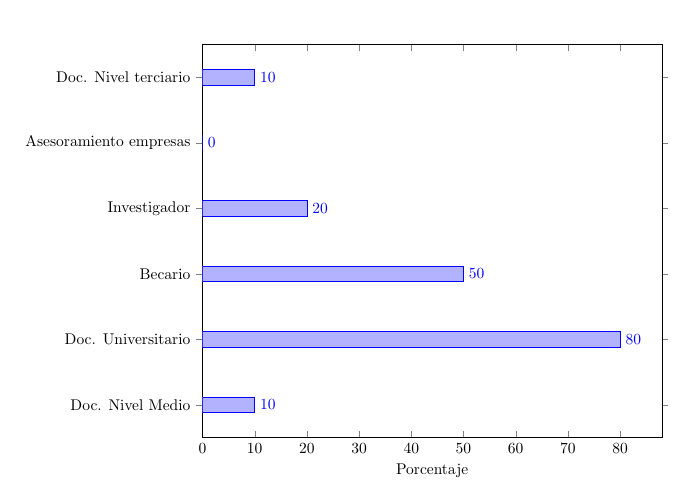
\includegraphics[scale=.5]{barras8.png}



\paragraph{Resultado encuesta a graduados (Persona) }
\paragraph{Aspiración }
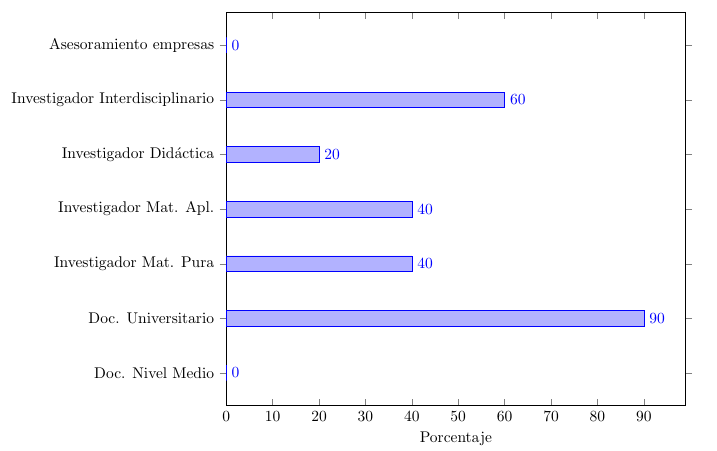
\includegraphics[scale=.5]{barras9.png}

Predilección por ocupaciones académicas!

Efectividad carrera para aspiraciones promedio: 7.6 (del 1 al 10)




\paragraph{Resultado encuesta a graduados (Persona)}
\paragraph{Relación con el profesorado }
\includegraphics[scale=.4]{torta3.png}

Valoración positiva ciclo común promedio: 9 



\paragraph{Resultado encuesta a graduados (Enseñanza)}
\paragraph{Relaciones entre asignaturas}

A veces:9,   N/C: 1.


 \includegraphics[scale=.3]{barras1.png}








\paragraph{Resultado encuesta a graduados (Enseñanza)}
\paragraph{Espacios Interdisciplinarios}

Hay: 5, No hay: 4,  N/C: 1.


 \includegraphics[scale=.5]{barras2.png}
 
 Suficiencia de los espacios promedio: 3.5 (del 1 al 10)








\paragraph{Resultado encuesta a graduados (Enseñanza)}
\paragraph{Acercamiento campo profesional}

Hay: 6, No hay: 3,  N/C: 1.

\begin{center}
  \includegraphics[scale=.5]{barras3.png}
\end{center}


 






\paragraph{Resultado encuesta a graduados (Enseñanza)}
\paragraph{Buena articulación Teoría-Práctica}

\begin{center}
  \includegraphics[scale=.5]{torta4.png}
\end{center}


 








\paragraph{Resultado encuesta a graduados (Enseñanza)}
\paragraph{ Utilidad para la formación de la metodología de evaluación}
\begin{center}
  \includegraphics[scale=.5]{torta5.png}
\end{center}








\paragraph{Resultado encuesta a graduados (Competencias)}
%\paragraph{Acercamiento campo profesional}



\begin{center}
 \includegraphics[scale=.5]{barras4.png}
\end{center} 







\paragraph{Resultado encuesta a graduados (Competencias)}
\paragraph{Acercamiento campo profesional}




\begin{center}
 \includegraphics[scale=.5]{barras5.png}
 
\end{center} 








\paragraph{Resultado encuesta a graduados (Contenidos)}
\paragraph{Acercamiento campo profesional}




\begin{center}
 \includegraphics[scale=.5]{barras6.png}
 \end{center} 







\paragraph{Resultado encuesta a graduados (Contenidos)}
\paragraph{Acercamiento campo profesional}




\begin{center}
 \includegraphics[scale=.6]{barras7.png}
 
 \end{center} 








\paragraph{Mapeo Teorías matemáticas}
 
 
\begin{center}
 \includegraphics[scale=.2]{dependencias2.pdf}
% \includegraphics[scale=.25]{mapeo.png}
\end{center}







\paragraph{Como seguir?}
\paragraph{Definir Perfil}
 \smartdiagramset{
 planet size=3cm,
 planet text width=2cm,
 planet font=\footnotesize,
 satellite size=1cm, 
 satellite text width=1.5cm,
 satellite font=\scriptsize,
 distance planet-text=0,
 %distance satellite-text=0,
 distance planet-satellite=3.5cm,
 /tikz/connection planet satellite/.append style={<-}
 } 
 
 \begin{center}
 \scalebox{0.8}{
 \smartdiagram[constellation diagram]{
  Perfil,
  Epistemología, 
  Optimización,
  Modelización,
  Enseñanza,
  Progr. Algorit.,
  DD.HH,
  Análisis datos,
  Resolver Prob.,
  Investigar,
  etc}}
  \end{center}






\bibliographystyle{apalike} 
\bibliography{BaseBibliografia,Geometria,Modelos}




\end{document}
